%\documentclass[notes]{beamer}       		% compila sia i frame che le note
\documentclass{beamer}              				% compila solo i frame
%\documentclass[notes=only]{beamer}  	% compila solo le note

% ita language and encoding
\usepackage[utf8]{inputenc}
%\usepackage[italian]{babel}

% formattazione
\usepackage{ragged2e} 							% pacchetto che contiene il comando \justifying
%\apptocmd{\frame}{}{\justifying}{}  	% --> applica la giustificazione a tutti i frame del documento
%\justifying											% --> applica la giustificazione a tutto il documento

% graphics style
\usepackage{graphicx}
\usepackage{xcolor}
\usepackage{shadowtext}

%image paths
\graphicspath{{./Immagini/}{./Immagini/TRD/}{./Immagini/ToF/}}

% impostazioni base delle slide - tema, colori, caratteri, ... (deic.uab.es/~iblanes/beamer_gallery/)
\mode<presentation>
{
	\usetheme{CambridgeUS}      % or try Darmstadt, Madrid, Warsaw, ...
  	\usecolortheme{rose} 			% or try albatross, beaver, crane, orchid, rose ...
	\usefonttheme{structurebold} % or try structureitalicserif, structuresmallcapsserif
}

% settagio dati principali del file - titolo, autore, ...
\title[Presentation on the AMS-02 experiment]{The AMS-02 experiment}
\subtitle{General review of the apparatus}
\author{Daniele Di Bari}
\institute{University of Perugia}
\date{27th April 2017}
\subject{Course of Particle Detectors}

% By default the beamer class adds navigation buttons in the bottom right corner. To remove them one can place
\beamertemplatenavigationsymbolsempty

% settaggio prima slide
\setbeamertemplate{title page}
{
	\shadowcolor{white!30!black}
	\vspace{-0.5cm}	
	
    \shadowtext{\textcolor{white}{\textbf{\footnotesize{The Alpha Magnetic Spectrometer}}}}
   
    \vspace{0.15cm}  	
    
   	\shadowtext{\textcolor{white}{\textbf{\LARGE \inserttitle}}}\par
      
   	\vspace{0.1cm}  

   	\shadowtext{\textcolor{white}{\emph{\large \insertsubtitle}}}\par
   	
   	\vspace{2.5cm}
	
	\titlepagetext{lightgray}{The general particle physics}\\
	\titlepagetext{lightgray}{experiment in space, on board}\\
	\titlepagetext{lightgray}{the International Space Station}\\
	\titlepagetext{lightgray}{since 19th May 2011.}		
}
				
% colors
\definecolor{itemred}{RGB}{163,0,0}
\definecolor{itemblue}{RGB}{52,57,176}

% COMANDI
% Formato testo generico in titolpage
\newcommand\titlepagetext[2]{\textcolor{#1}{\footnotesize{\textit{{#2}}}}}
\newcommand\colortextbf[2]{\textcolor{#1}{\textbf{#2}}}
\newcommand\bluetextbf[1]{\textcolor{itemblue}{\textbf{#1}}}
\newcommand\bluetextit[1]{\textcolor{itemblue}{\textit{#1}}}
\newcommand\textitem[2]{\textcolor{itemblue}{\textbf{#1} (\textit{#2})}}

% Testo giustificato
\newenvironment<>{justify}{\justifying{}}


% 	MODIFICA DEL TEMA CambridgeUS -- HEAD AND FOOTLINES
%		Il tema CambridgeUS usa il outer-tema "infolines" outer theme che imposta head and footlines (vedi il file .sty: ../tex/latex/beamer/themes/theme/beamerthemeCambridgeUS.sty). 
%		Ad esempio, in "beamerouterthemeinfolines.sty" è definito il "footline template" in cui sono dichiarate tre caselle - la prima per l'autore, la seconda per il titolo e l'ultima per la data e il numero.
%		Utilizzo delle impostazioni di base di "infolines" e modificando diversi parametri per ottenere il layout il tema personalizzato
\setbeamercolor{institute in head/foot}{parent=palette secondary}
\setbeamercolor{subject in head/foot}{parent=palette tertiary}
\setbeamercolor{title in head/foot}{parent=palette primary}
\setbeamertemplate{footline}
{
	\leavevmode%
	\hbox{%
  		% "ht" è lo spazio sopra il carattere partendo dalla base del carattere, "dp"  è lo spazio sotto il carattere partendo sempre dalla base del carattere
  		\begin{beamercolorbox}[wd=.333333\paperwidth,ht=2.5ex,dp=1ex,left,leftskip=4ex]{author in head/foot}%
   			\usebeamerfont{author in head/foot}\insertshortauthor
  		\end{beamercolorbox}%
  		\begin{beamercolorbox}[wd=.333333\paperwidth,ht=2.5ex,dp=1ex,center]{institute in head/foot}%
    		\usebeamerfont{title in head/foot}\insertshortinstitute
 		 \end{beamercolorbox}%
 		 \begin{beamercolorbox}[wd=.333333\paperwidth,ht=2.5ex,dp=1ex,right,rightskip=4ex]{date in head/foot}%
 		 	\usebeamerfont{date in head/foot}\insertshortdate{}\hspace*{2em}\insertframenumber{} / \inserttotalframenumber
 		 \end{beamercolorbox}
 		 }%
 	\vskip0pt%
}
\makeatletter
\setbeamertemplate{headline}
{
  \leavevmode%
  \hbox{%
  \begin{beamercolorbox}[wd=.5\paperwidth,ht=2.8ex,dp=1.35ex,left]{subject in head/foot}	
    \usebeamerfont{section in head/foot}\hspace*{4ex}Course of Particle Detectors			% --> N.B. Qui c'è l'unica scritta che non usa nessun template tipo \title o \institute
  \end{beamercolorbox}%
  \begin{beamercolorbox}[wd=.5\paperwidth,ht=2.8ex,dp=1.35ex,right]{title in head/foot}%
    \usebeamerfont{subsection in head/foot}\insertshorttitle\hspace*{4ex}
  \end{beamercolorbox}}%
  \vskip0pt%
}
\makeatother
%\makeatletter
%\setbeamertemplate{headline}
%{
%  \leavevmode%
%  \hbox{%
%  \begin{beamercolorbox}[wd=.5\paperwidth,ht=2.65ex,dp=1.5ex,right]{subject in head/foot}%
%    \usebeamerfont{section in head/foot}\expandafter\beamer@ifempty\expandafter{\insertsectionhead}{Course of Particle Detectors}{\insertsectionhead}\hspace*{2ex}
%  \end{beamercolorbox}%
%  \begin{beamercolorbox}[wd=.5\paperwidth,ht=2.65ex,dp=1.5ex,left]{title in head/foot}%
%    \usebeamerfont{subsection in head/foot}\hspace*{2ex}\expandafter\beamer@ifempty\expandafter{\insertsubsectionhead}{\insertshorttitle}{\insertsubsectionhead}
%  \end{beamercolorbox}}%
%  \vskip0pt%
%}
%\makeatother
%% FINE MODIFICA

\begin{document}
	% impostare una foto come sfondo del frame: 
	\usebackgroundtemplate{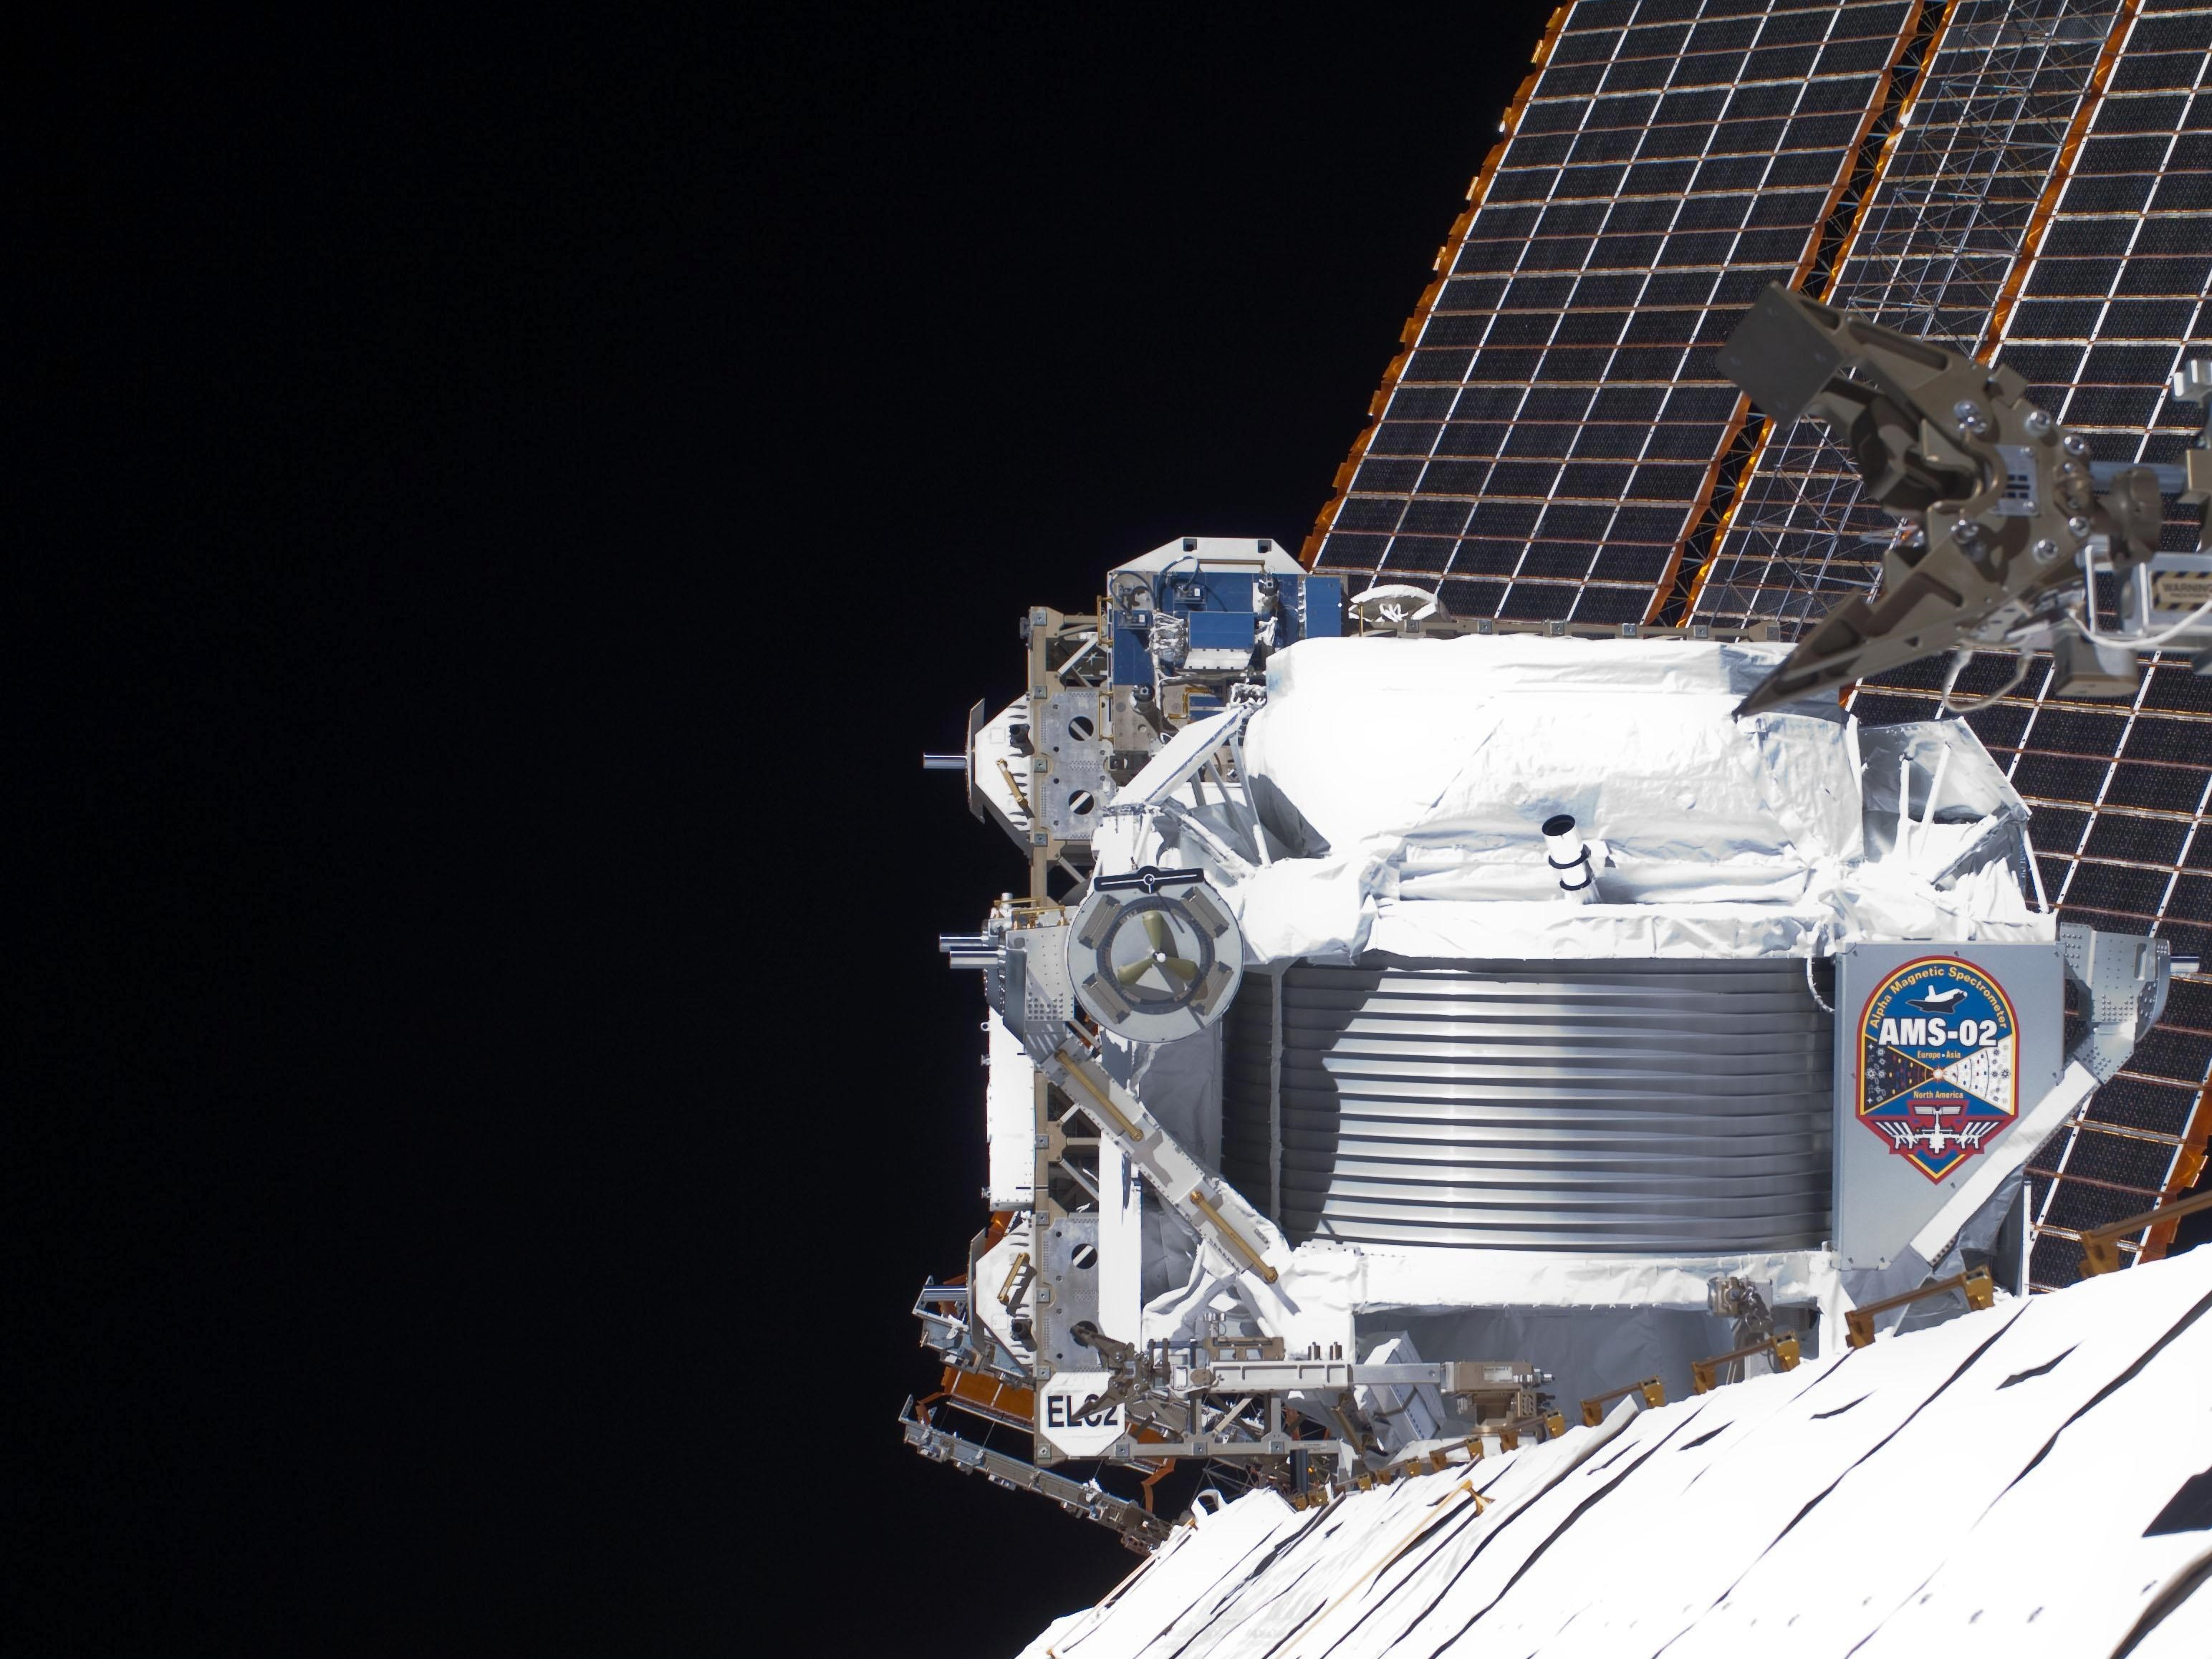
\includegraphics[height=\paperheight,keepaspectratio]{on_ISS-08_cutMIDDLEUP-3088.jpg}}	
	% 	possibili impostazioni per l'img: width=\paperwidth  --  height=\paperheight  --  keepaspectratio

\begin{frame}
	\titlepage
\end{frame}

\note{ 
\footnotesize{
The absorption thickness of the Earth's atmosphere, corresponding to an average of 25 radiation lengths (X0), screens the ground from primary CRs, which interact before reaching the detector. 

Direct detection of electromagnetically interacting CRs is therefore carried in space. In order to identify the nature of the detected particles, space borne instruments exploit typical high energy physics detection techniques, like um precision tracking using silicon detector technology or calorimetric energy measurements. 

Despite the detection concept is very similar to the modern accelerator experiments, the technological realization differs significantly. The requirements of a space borne experiment are in fact very challenging. Weight, dimension and power consumption constraints limit the size of the detector (thus their acceptance) to the $\sim$ 10 m$^3$ range. The limited bandwidth for the data transfer (to ground), the extreme thermal environment and the transport from ground to space also shape critically the detector concept.

In a typical direct CR detection experiment, particles traversing the instrument are fully characterized via the simultaneous measurement of the energy E, mass M, charge Z and charge sign. In a minimalistic experiment, a calorimeter is used to measure the energy E, dE=dX detectors are used to measure Z and a time of flight system is used to trigger the data acquisition and to measure the velocity and hence the mass M. A magnet can be used to detect the particle trajectory and infer the charge sign.

Some experiments are also equipped with additional detectors dedicated to the identification of CR rare species, like transition radiation detectors or neutron detectors that improve the identification of $e^{\pm}$. The measurement of CRs in space began in the 1970s with the measurement of nuclear isotopes in the energy range $\leqslant$ 1 GeV with the IMP satellites. The field flourished in 2000s, when the FERMI-LAT satellite observatory provided for the first time high precision rays direct measurements and the PAMELA satellite mission (see Figure 1.8) provided the direct measurement of charged CRs up to the 100 GeV range. The state-of-the-art space born experiment is the AMS-02 detector. AMS is the first particle detector located on the International Space Station (ISS) where it has been collecting high precision data up to the TeV range since 2011. The AMS detector will be exhaustively described in Chapter 2.

AMS successfully confirmed the possibility of operating a particle physics detector on the ISS, hence stimulating the development of the next (and ``next-to-next'') generation experiments to be operated on space stations, like the JEM-EUSO observatory or the DAMPE/HERD instrument.
}
}

\usebackgroundtemplate{}

\begin{frame}
\frametitle{Table of Contents}
\tableofcontents
\end{frame}

\begin{frame}<presentation:0>[noframenumbering]
	\frametitle{Technical Question about the Detector}
	AMS is a particle physics experiment in space, so it focuses on the detection of particles, but:
	\begin{itemize}
	\item	Which kind of particle do we have to detect?
	\item	What is the required dimension of the detector?
	\item	Which ``property'' of the particle do we have to know?
	\begin{itemize}
		\item[$\circ$]	Position - Trajectory
		\item[$\circ$]	Time
		\item[$\circ$]	Number
		\item[$\circ$]	Energy
		\item[$\circ$]	Momentum
	\end{itemize}
	\item	What is the required resolution?
	\item	What is the maximum count rate?
	\item	What is the time distribution of the events?
	\item	And last, but not least, how much does it cost? 
	\end{itemize}
\end{frame}

\section{Introduction}
\begin{frame}
	\setbeamertemplate{background}{white}
	\frametitle{Introduction}
	\framesubtitle{The Alpha Magnetic Spectrometer}
	\justifying
	AMS-02 is a general purpose \textbf{high energy particle detector}  designed to operate as an external module on the
	International Space Station.
	
	\vspace{0.25cm}
	\begin{block}{Purpose of the AMS experiment}
		\justifying
		To perform accurate, high statistics, long duration measurements of the spectra of energetic primary charged 
		cosmic rays (CRs) in space. 
	\end{block}
		
	\vspace{0.25cm}
	Some of the \textbf{physics goals} are:
	\begin{enumerate}
		\item \bluetextbf{Dark Matter}
		\item \bluetextbf{Matter/Antimatter Asymmetry}
		\item \bluetextbf{Cosmic Ray Physics}
	\end{enumerate}
\end{frame}
\note{
	AMS-02 (Alpha Magnetic Spectrometer ) is a general purpose high energy particle detector which was successfully deployed on 
	the International Space Station (ISS) on May 19, 2011 to conduct a unique long duration mission of fundamental physics 
	research in space. Among the physics objectives of AMS are the searches for an understanding of Dark Matter, Anti-matter, the 
	origin of cosmic rays and the exploration of new physics phenomena not possible to study with ground based experiments
	Lo scopo dell'esperimento è quello di effettuare, per un periodo di lunga durata così da ottenere un'elevata statistica, delle 
	misure molto accurate dello spettro di energia (per energie fino all'ordine dei TeV) dei raggi cosmici carichi primari direttamente 
	nello spazio.
}

\section{Technical Requirements}
\subsection{from Physics Goals}
\begin{frame}
    \frametitle{Technical Requirements}
    \framesubtitle{from Physics Goals}
    \justifying
    
	Physical goals involve \textbf{technical requirements for the AMS detector}:
	
	\begin{itemize}\justifying
		\item	\bluetextbf{Dark Matter $\Rightarrow$}
					to get $e^+/p$ rejection of $\sim10^{-6}$ for the measurement of the positron fraction.
		\item	\bluetextbf{Matter/Antimatter Asymmetry $\Rightarrow$}
					to reach a sensitivity in the search for anti-matter nuclei of $10^{-10}$ (ratio of anti-helium nuclei to helium nuclei).
		\item	\bluetextbf{Cosmic Ray Physics $\Rightarrow$}
					to measure the composition and spectra of charged particles with an accuracy of 1\%.
	\end{itemize}
	
	Moreover, \bluetextbf{for each of these ones}, it is very important to extend, as far as possible, the energy range of the 
	measurements.
	
	For AMS, the required energy range is from 0.5 to $\sim$ 2000 $GeV$.

	%\footnotesize{\underline{\textbf{Note}} These requirements represent a considerable sensitivity improvement compared to the previous space-borne experiments.}

\end{frame}

\note{
	Esiste un forte interesse nell'effettuare delle misure di precisione della frazione di positroni dei raggi cosmici nella regione 
	energetica da 10 a 1000 GeV, in quanto le misurazioni di $e^+ / (e^+ + e^-)$, da AMS-01, HEAT, PAMELA e FERMI indicano 
	una grande deviazione di questo rapporto dalla produzione di e+ e e- previsto da un modello che comprende solo collisioni 
	ordinarie del raggio cosmico.
   	 
   	These available measurements are both at too low an energy and of too limited statistics to shed the light on the origin of this 
   	significant excess.
   	 
	AMS-02 is expected to provide definitive answers concerning the nature of this deviation.
}

\begin{frame}
	\frametitle{Technical Requirements}
    \framesubtitle{from Physics Goals}	
    
    \begin{block}{The technical challenge of AMS-02}
		\justifying
		The illustrated requirements represent a considerable sensitivity improvement compared to the previous space-borne 
		experiments.
	\end{block}
   	
   	\vspace{0.25cm}
	\small{\bluetextbf{NOTE}}
	\vspace{-0.2cm}
    \begin{itemize}
    	\item[\footnotesize{$\blacktriangleright$}] 
    		\footnotesize{\justifying
    		There is a strong demand for precision measurements of CRs in the energy region from 10 to 1000 
    		$GeV$ as the measurements of positron fraction, i.e.  $e^+ / (e^+ + e^-)$, by AMS-01, HEAT, PAMELA and FERMI 
    		indicate a large deviation of this ratio from the production of $e^+$ and $e^-$ predicted by a model that includes only 
    		ordinary CR collisions.
    		
    		These available measurements are both at too low an energy and of too limited statistics to shed the light on the origin of 
    		this significant excess.
    		
    		AMS-02 is expected to provide definitive answers concerning the nature of this deviation.}
   	\end{itemize}  
   	 
%
%%	\vspace{0.25cm}
%	There is a strong demand for precision measurements of cosmic rays in the energy region from 10 to 1000 GeV as the 
%	measurements of e+/(e+ + e-) by AMS-01, HEAT, PAMELA and FERMI indicate a large deviation of this ratio from the 
%	production of e+ and e- predicted by a model that includes only ordinary cosmic ray collisions. 
%	
%	These available measurements are both at too low an energy and of too limited statistics to shed the light on the origin of this 
%	significant excess. 
%	
%	AMS-02 is	expected to provide definitive answers concerning the nature of this deviation.
\end{frame}

%\begin{frame}
%	\frametitle{Technical Requirements}
%    \framesubtitle{From Physics Goals}
%	\begin{columns}
%		\begin{column}{0.5\textwidth}
%			\begin{center}
%				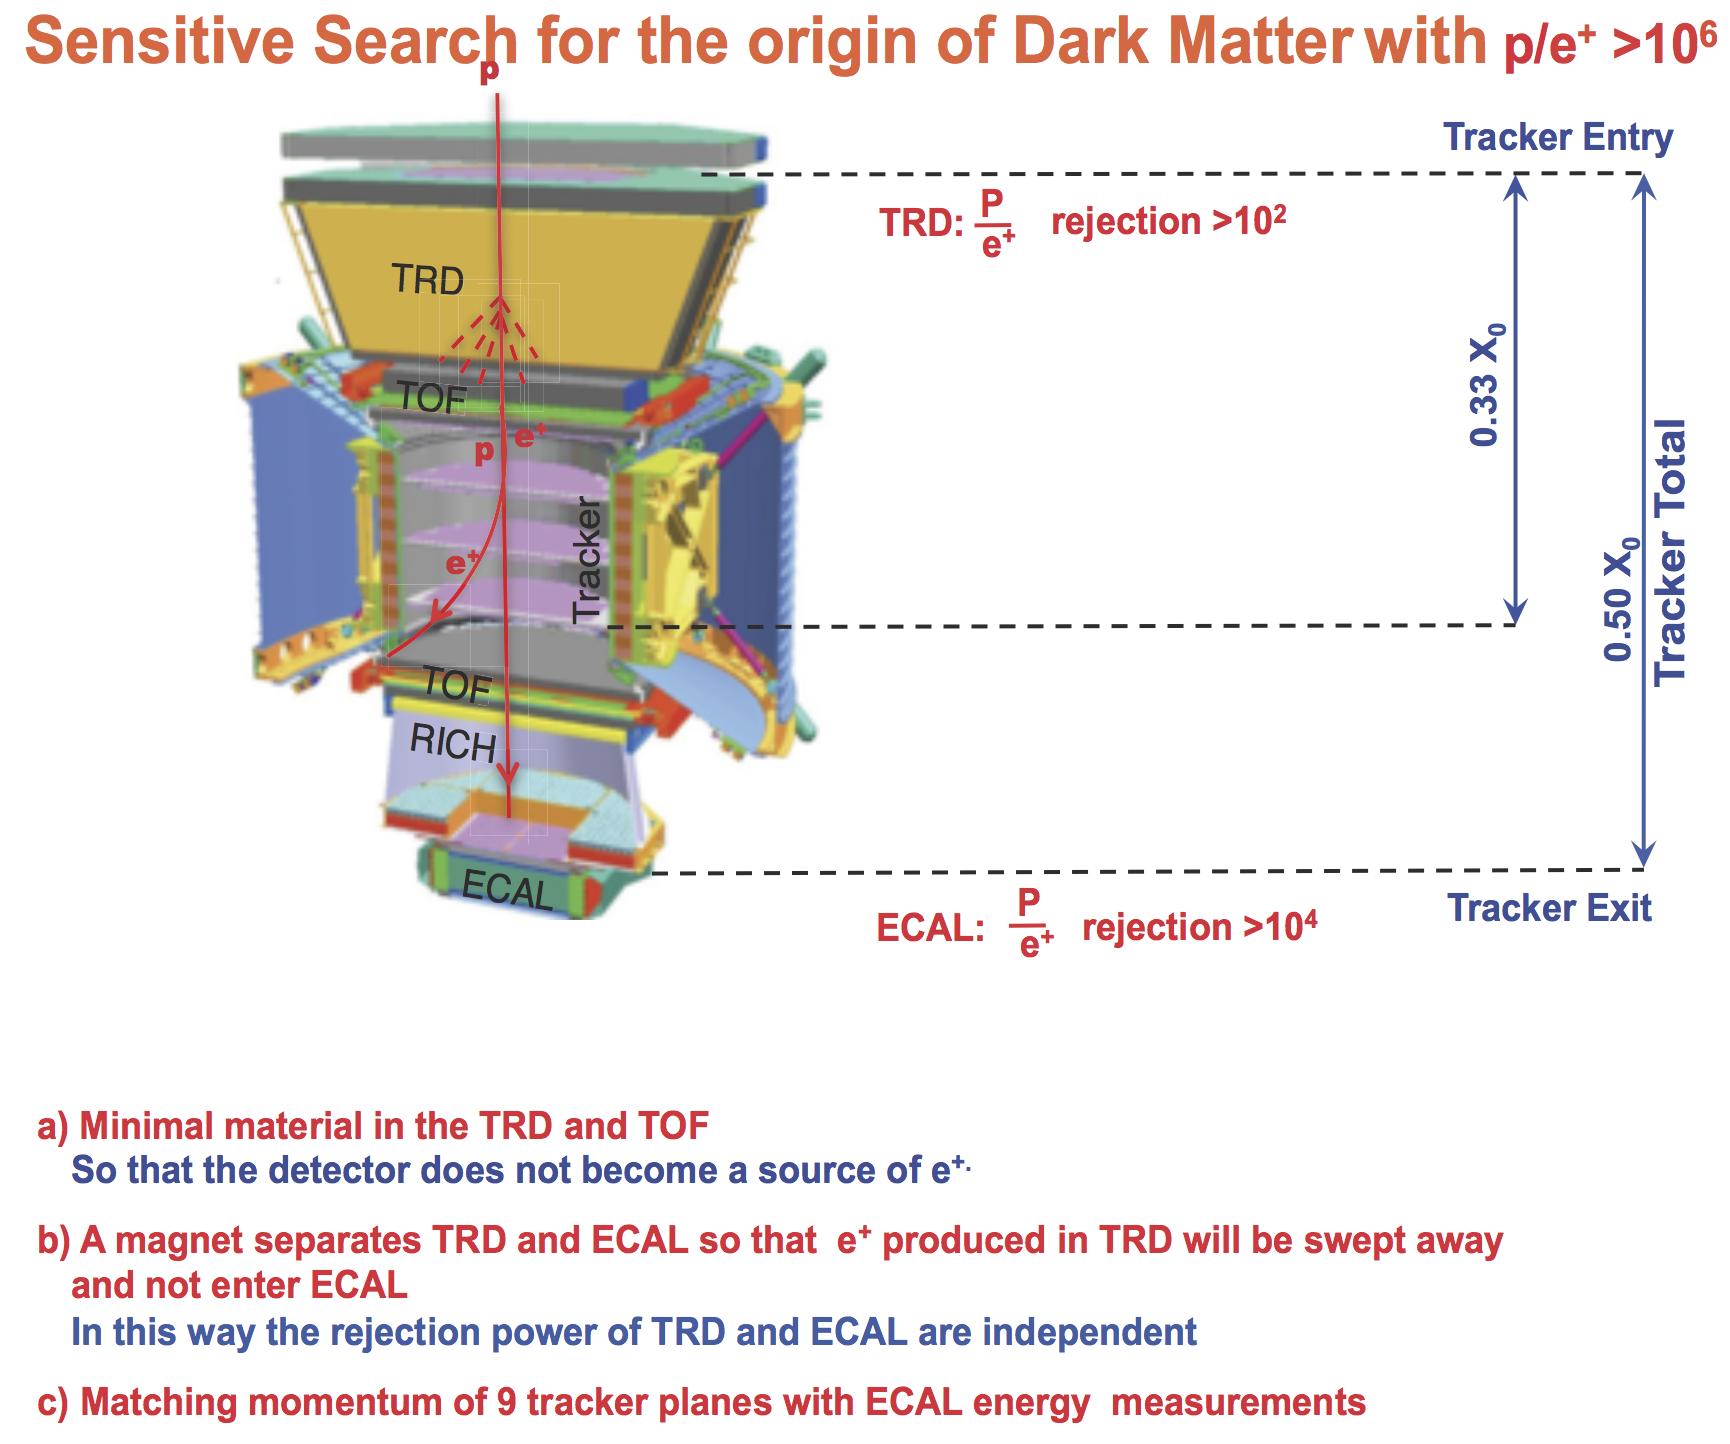
\includegraphics[width=0.95\columnwidth]{Schem_Requirements-DM.png}
%			\end{center}
%		\end{column}
%
%		\begin{column}{0.5\textwidth}
%			\begin{center}
%				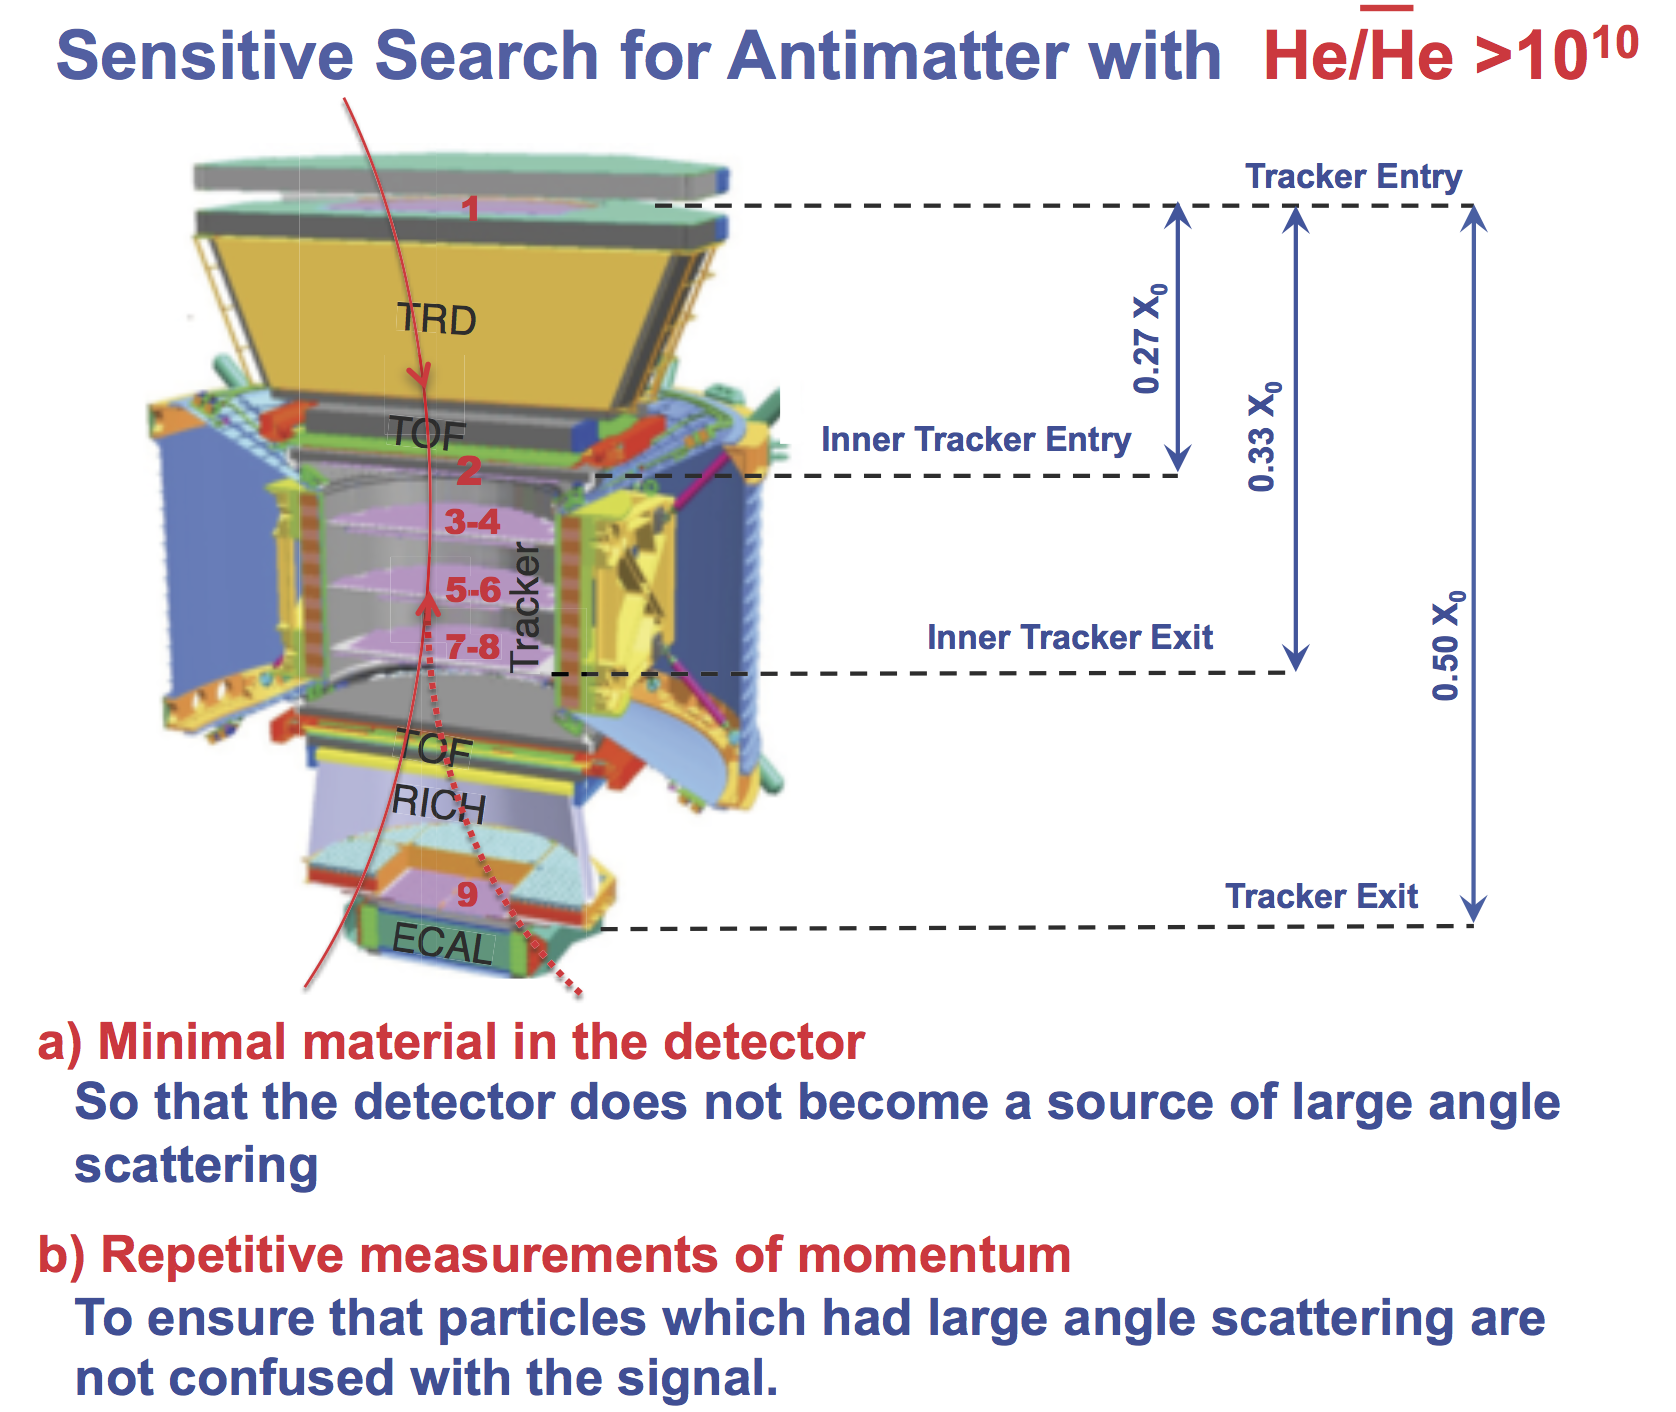
\includegraphics[width=0.95\columnwidth]{Schem_Requirements-Antimatter.png}
%			\end{center}
%		\end{column}
%	\end{columns}
%\end{frame}

\begin{frame}[label=AMS-apparatus_img]
	\frametitle{Technical Requirement}
	\framesubtitle{general structure of the AMS apparatus}
	\begin{center}
		\vspace{-0.15cm}
		\hspace{-0.35cm}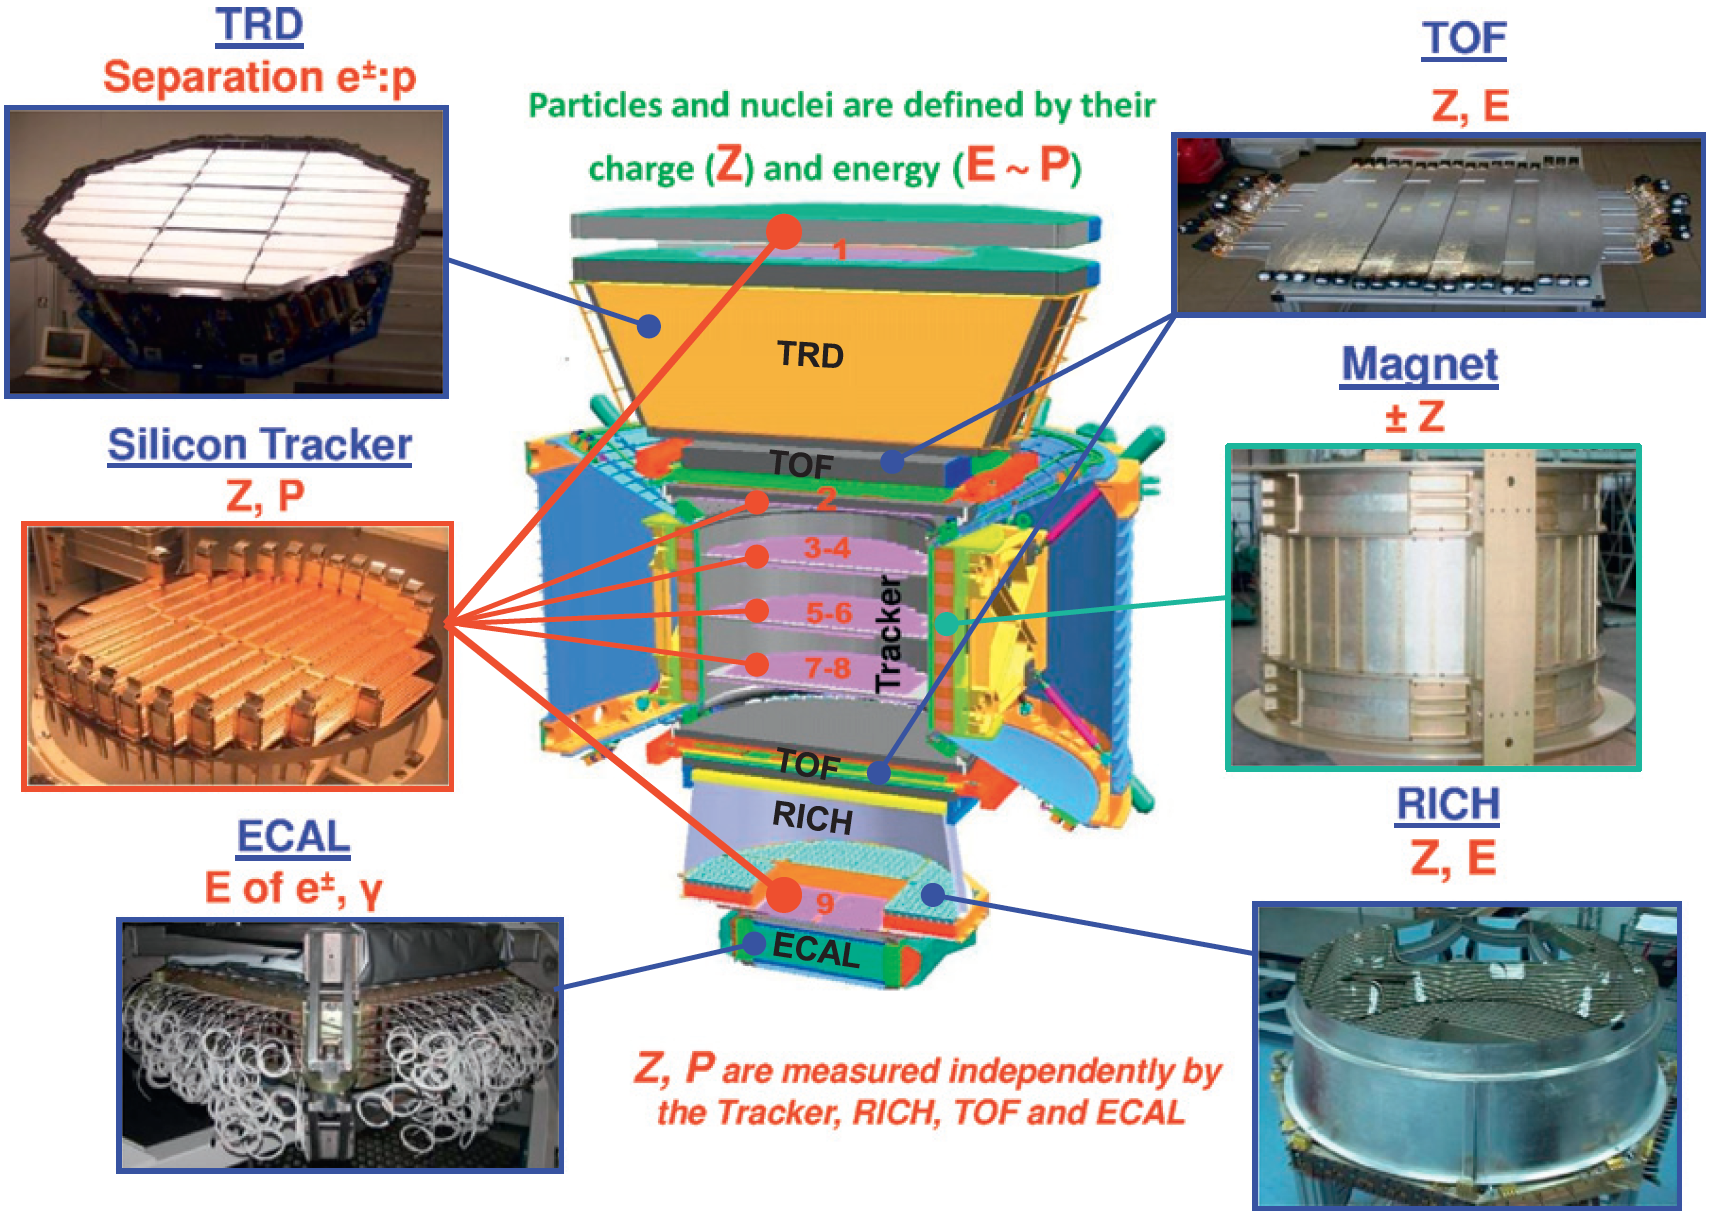
\includegraphics[height=0.7\paperheight]{Schem_structure_of_AMS.png}

		\vspace{-0.35cm}

		\hspace{0.25cm}\hyperlink{AMS-apparatus_list}{\textbf{\beamerbutton{link to AMS apparatus list}}}
	\end{center}
	%\vspace{-0.25cm}
\end{frame}

\begin{frame}
	\frametitle{Technical Requirement}
	\framesubtitle{from the research on the Dark Matter}
	\begin{center}
		\vspace{-0.1cm}
		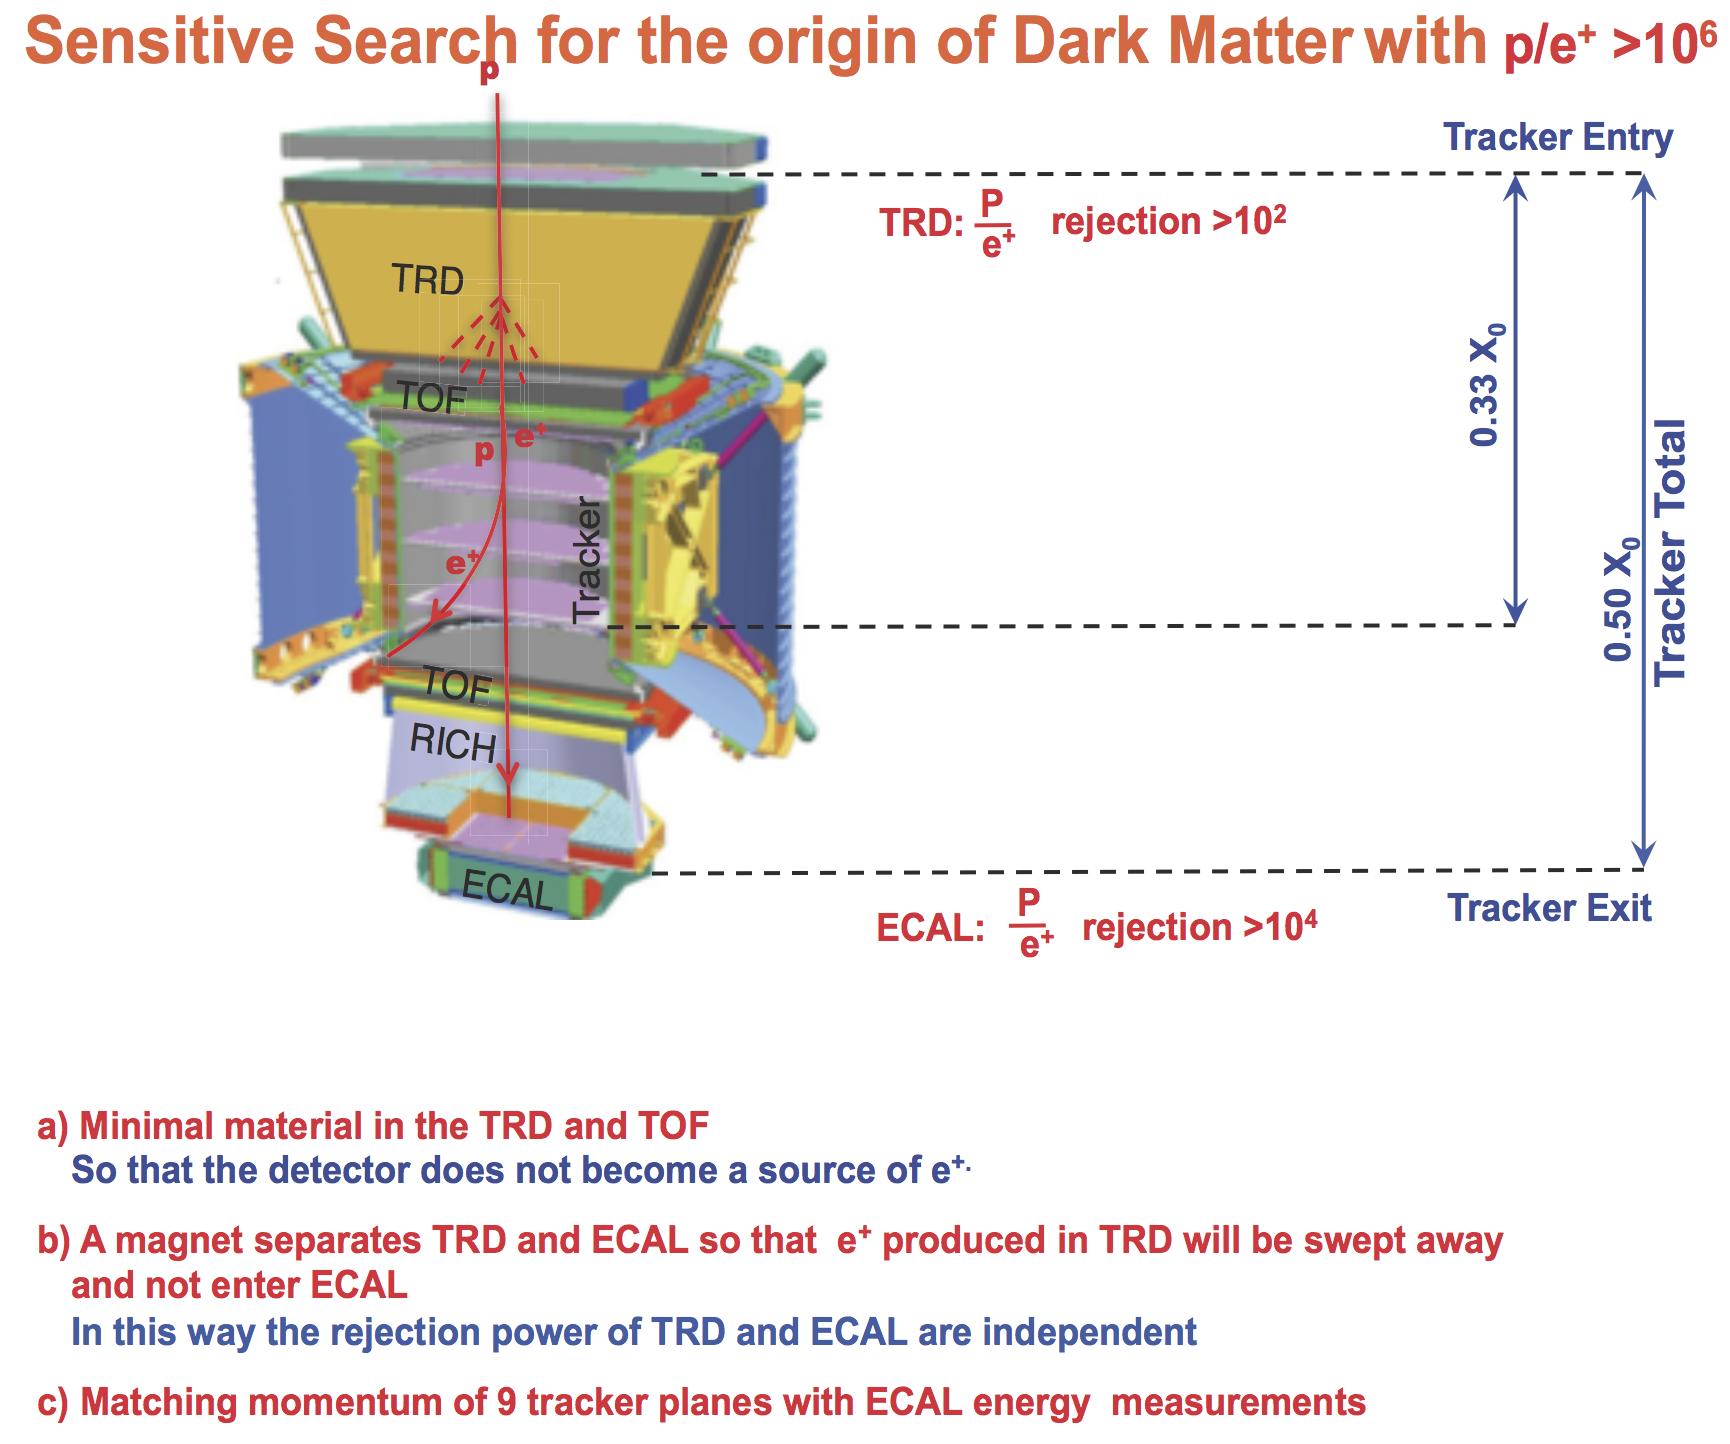
\includegraphics[height=0.72\paperheight]{Schem_Requirements-DM.png}
	\end{center}
\end{frame}

\begin{frame}
	\frametitle{Technical Requirement}
	\framesubtitle{from the research on the Matter/Antimatter Asymmetry}
	\begin{center}
		\vspace{-0.1cm}
		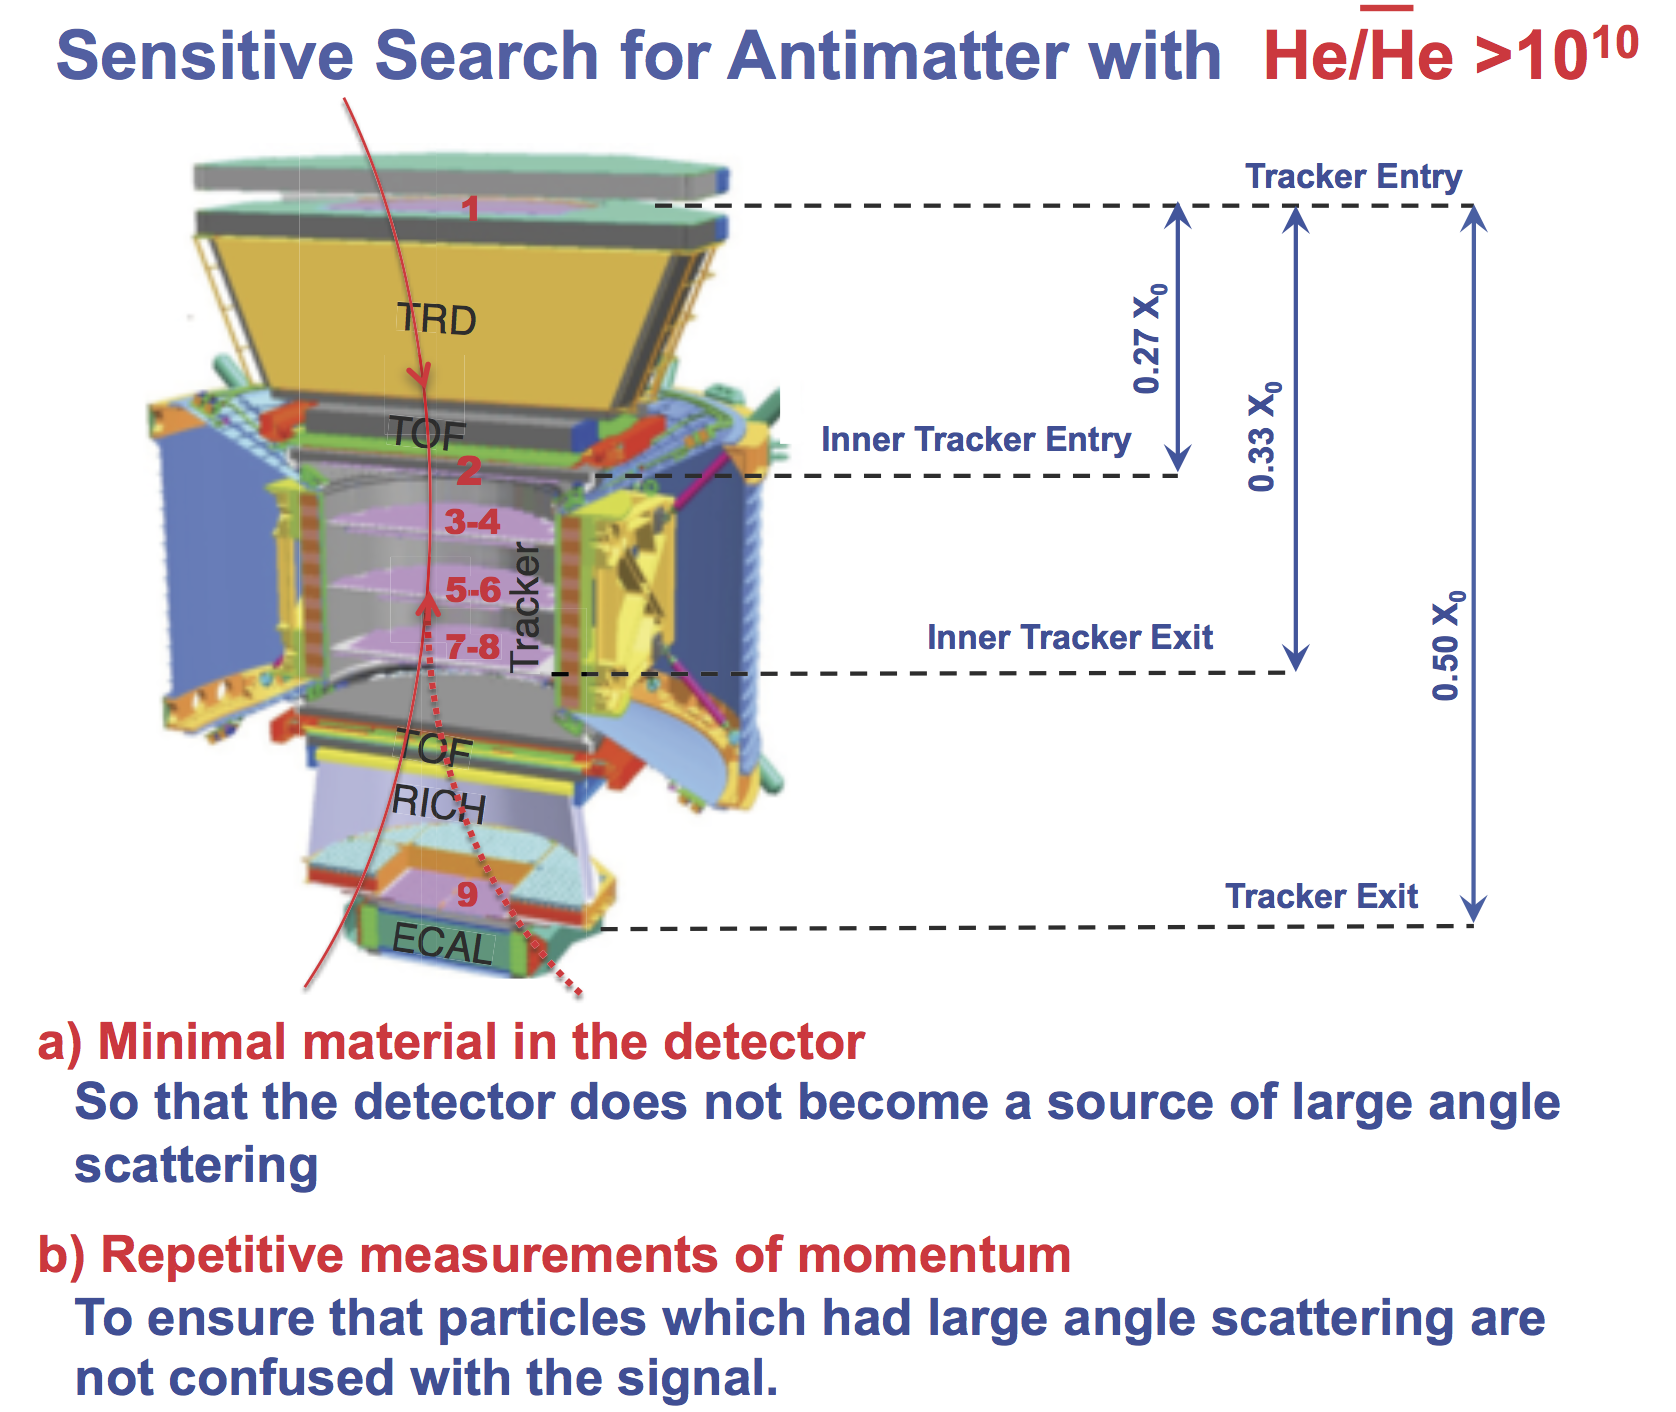
\includegraphics[height=0.65\paperheight]{Schem_Requirements-Antimatter.png}
	\end{center}
\end{frame}

\begin{frame}
	\frametitle{Technical Requirement}
	\framesubtitle{from the research on the Cosmic Ray}
	\begin{center}
		\vspace{-0.5cm}
		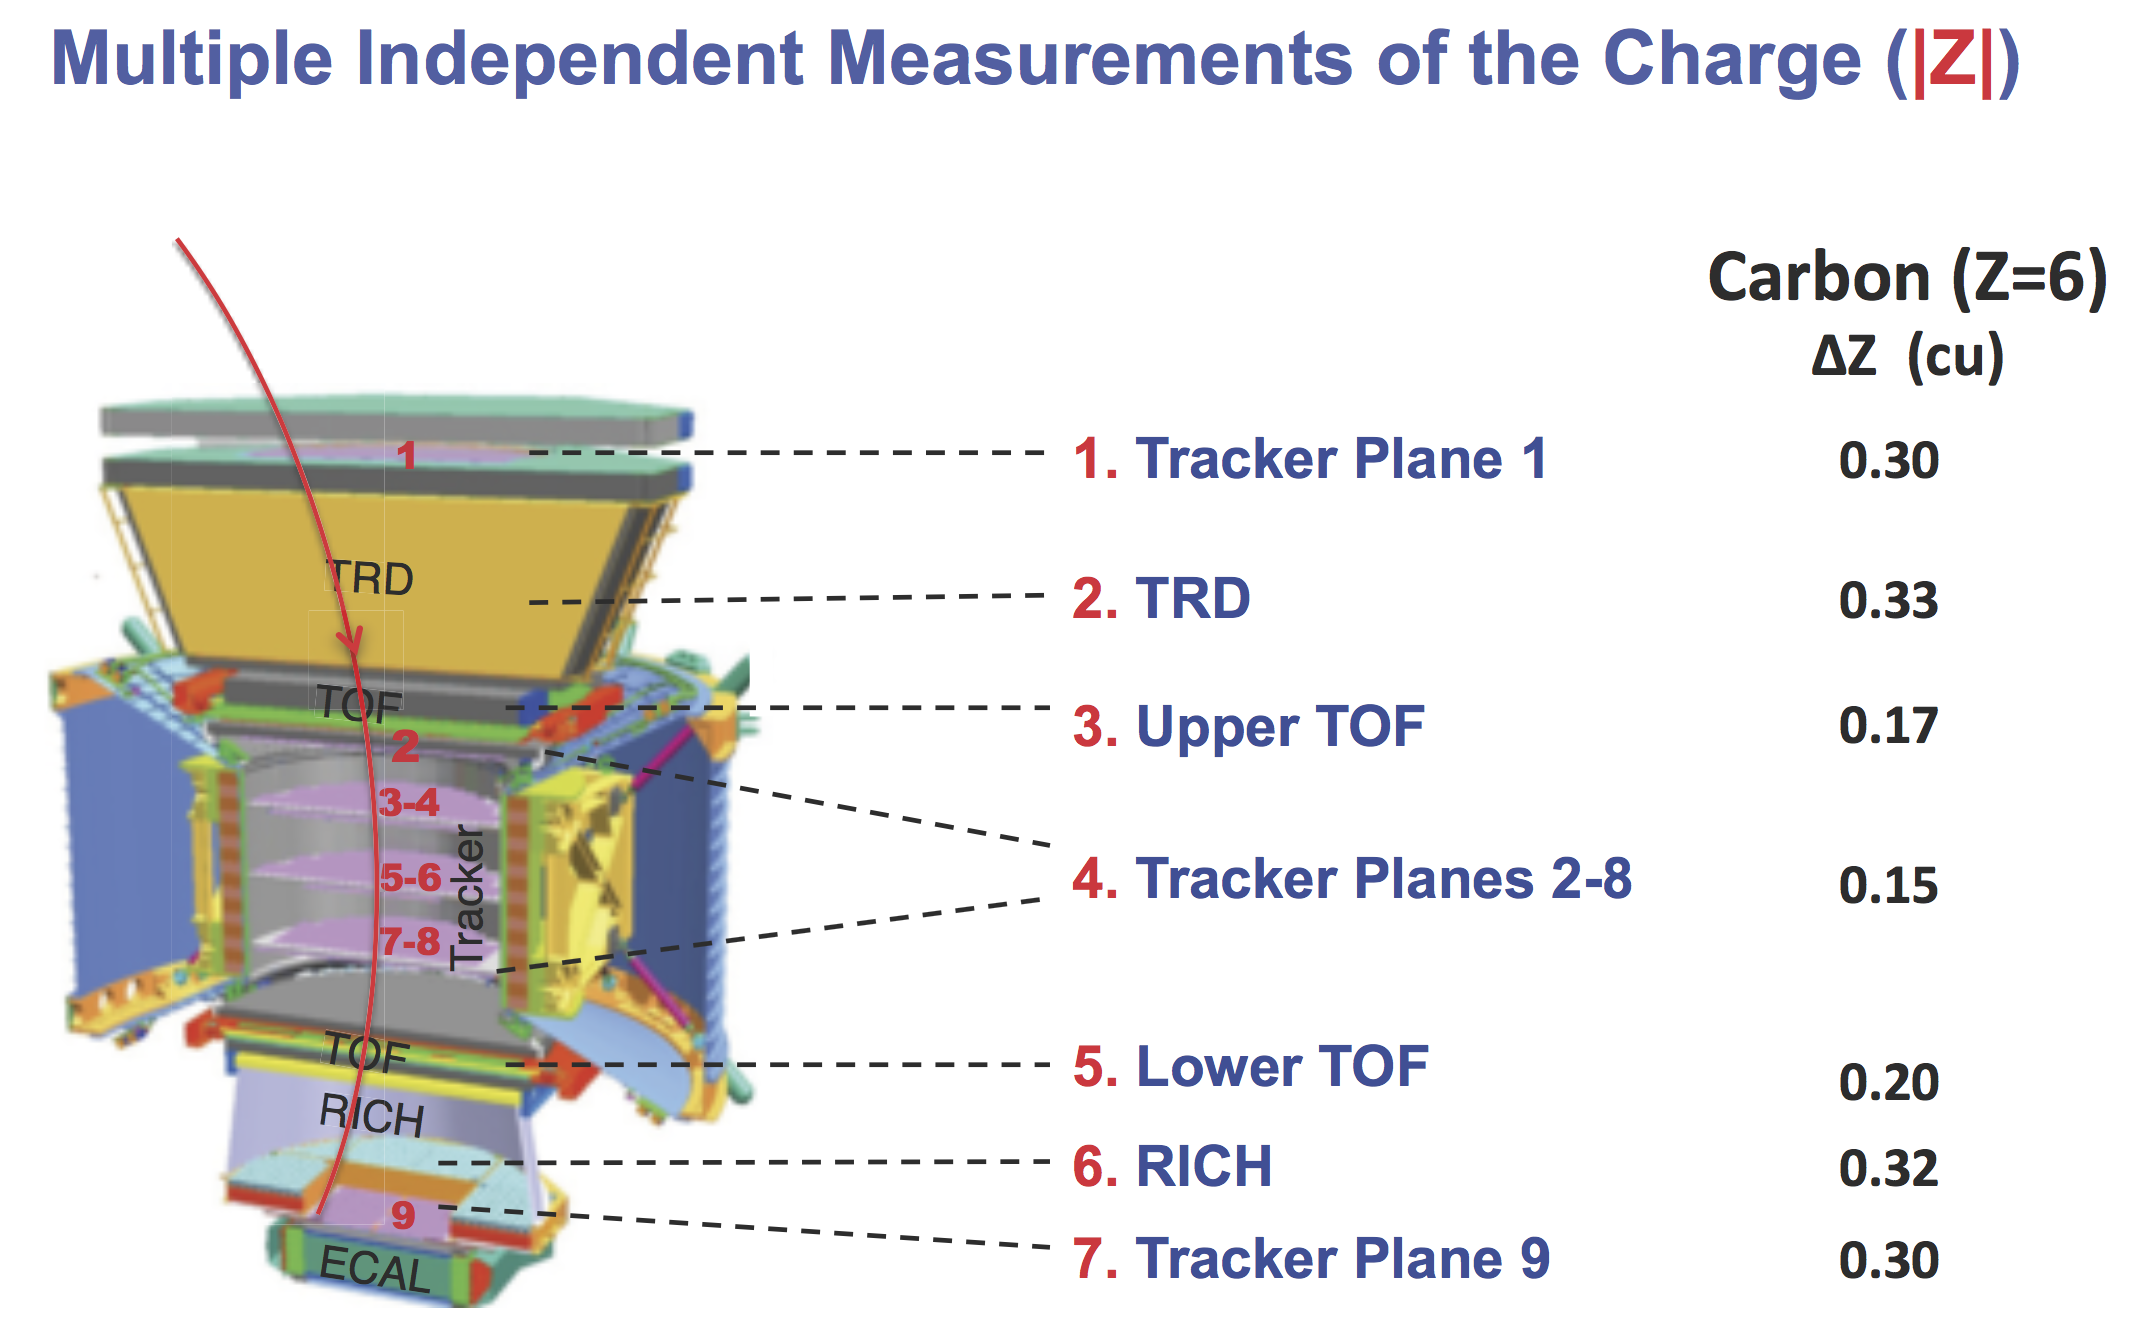
\includegraphics[height=0.55\paperheight]{Schem_Requirements-Charge02.png}
	\end{center}
\end{frame}

%\begin{frame}
%	\frametitle{Technical Requirement}
%	\framesubtitle{From the research on the Cosmic Ray}
%	\begin{center}
%		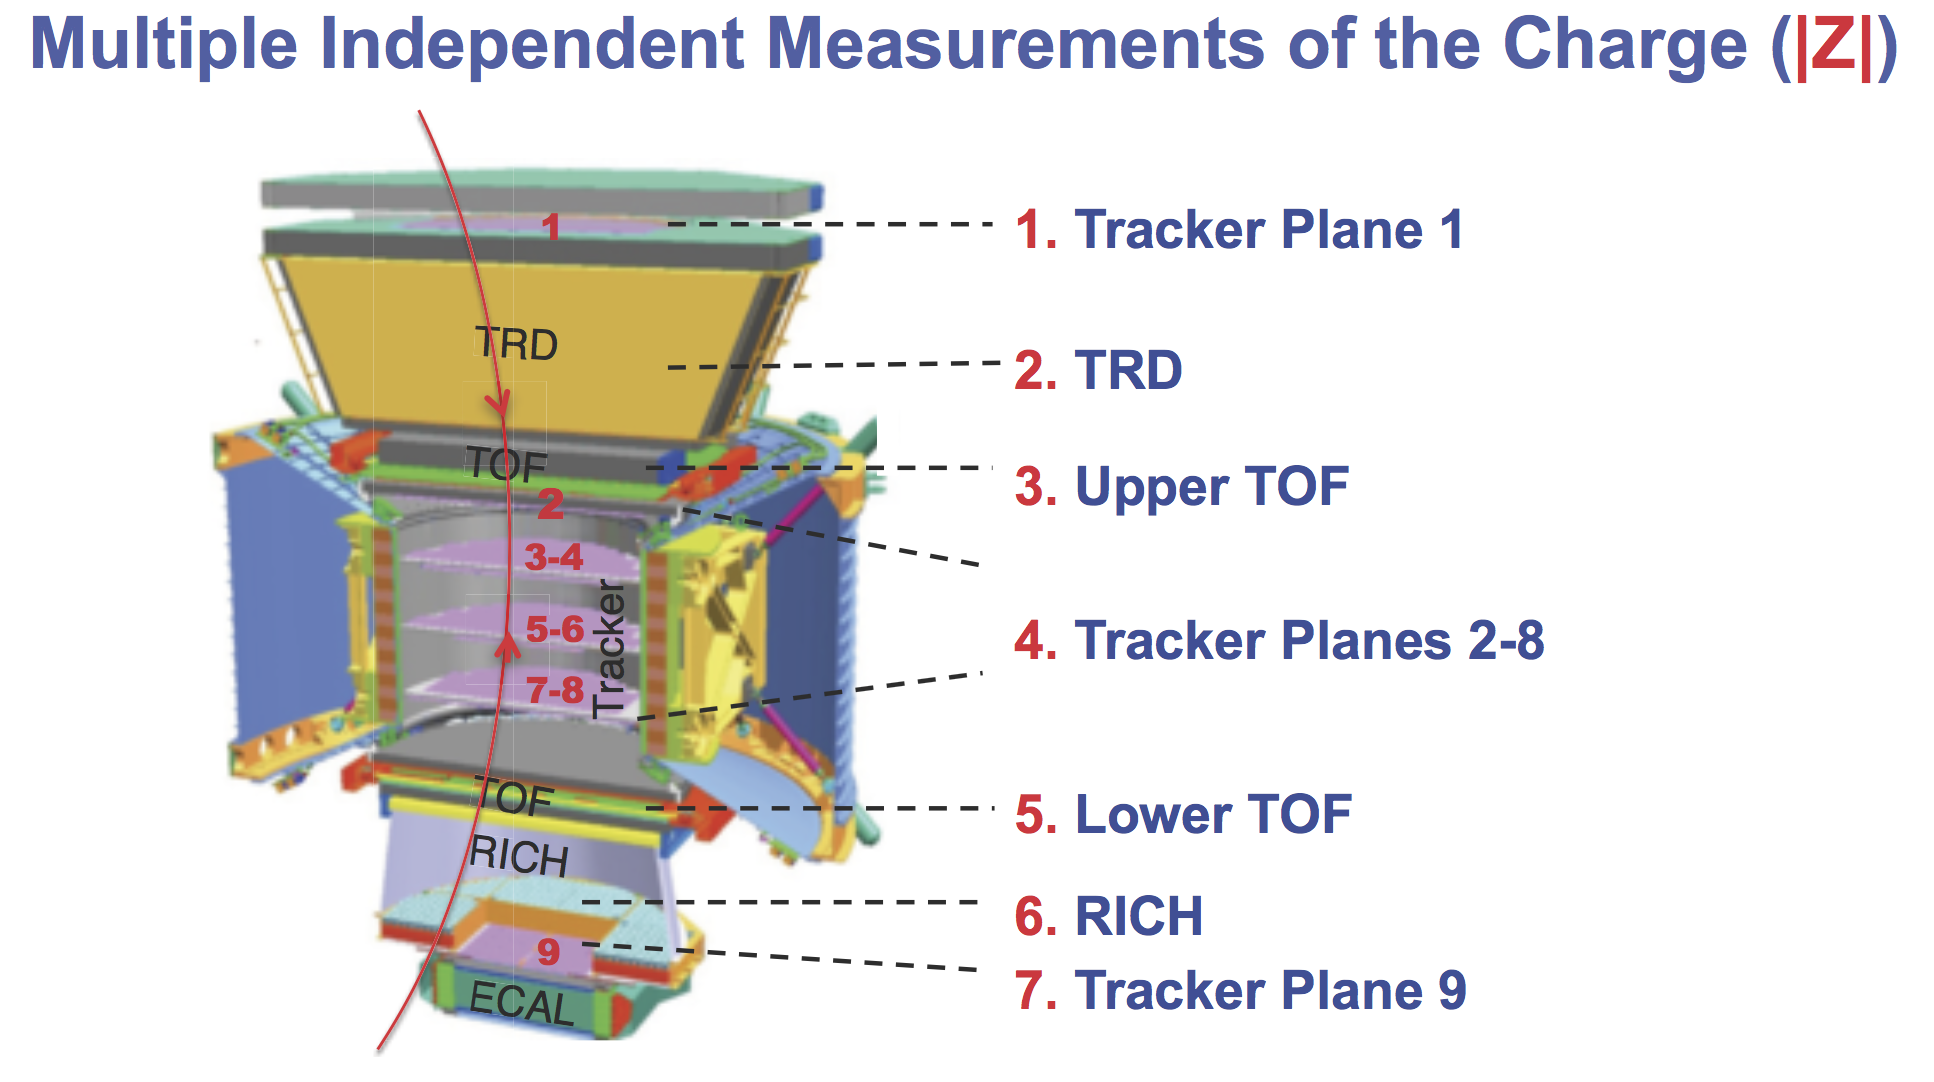
\includegraphics[height=0.5\paperheight]{Schem_Requirements-Charge.png}
%	\end{center}
%\end{frame}

\subsection{of a space-borne experiment}
\begin{frame}
	\frametitle{Technical Requirement} 
	\framesubtitle{why a particle detector in the space?}
	\justifying
	
	The absorption thickness of the Earth's atmosphere, corresponding to an average of 25 radiation lengths ($X_0$), screens the 
	ground from primary CRs, which interact before reaching the detector. 
	
	\vspace{0.25cm}
	\textbf{Direct detection of electromagnetically interacting CRs is therefore carried in space.} 
	
	\vspace{0.25cm}
	In order to identify the nature of the detected particles, space borne instruments exploit typical high energy physics detection 	
	techniques, like $\mu m$ precision tracking using silicon detector technology or calorimetric energy measurements. 

\end{frame}

\begin{frame}
	\frametitle{Technical Requirement} 
	\framesubtitle{of a space-borne experiment}
	\justifying
	
	\small{Despite the detection concept is very similar to the modern accelerator experiments, the technological realization differs 
	significantly.}
	
	\vspace{0.15cm}
	\small{\textbf{The requirements of a space borne experiment are in fact very challenging.}}
	
	\vspace{0.1cm}
	\begin{block}{The challenging requirements of a space born experiment}
		\justifying
		\small{
		Weight, dimension and power consumption constraints limit the size of the detector (thus their acceptance) to the 
		$\sim 10 m^3$ range.
		The limited bandwidth for the data transfer (to ground), the extreme thermal environment and the transport from ground to 
		space also shape critically the detector concept.
		
		Moreover, there is practically no way to fix any kind of problem with detectors and subsystem of AMS-02 once that it 
		is on the ISS\footnotemark[1].
%		Moreover, there is practically no way to fix any problem with AMS-02 detectors and subsystems when it's on the ISS
%		\footnotemark[1].
		}
	\end{block}
	
%	\footnotetext[1]{It is necessary a high degree of redundancy for the detector design to ensure that the functioning of the 
%	experiment remain on the required parameters for all the life time of the ISS (at least 20 years).}
	\footnotetext[1]{An high degree of redundancy in detector design is required to ensure that the operation of the experiment 
	remains within the required physical parameter for the entire lifetime of the ISS (at least 20 years)}
\end{frame}

%\begin{frame}
%	\frametitle{Technical Requirement} 
%	\framesubtitle{of a space-borne experiment}
%	New environment for HEP experiments
%	\begin{itemize}
%		\item	Operation in vacuum
%		\item	Acceleration during start and landing up to 9g
%		\item 	Temperature variations from $-180 \: ^\circ{C}$ to $+50 \: ^\circ{C}$
%		\item	Deposition limits on ISS $< 10^{-14} \frac{g}{s \cdot cm^2}$
%		\item	Weight limited to 13500 lb
%		\item	Datarate $1 Mbyte/s$ via 1 datalink
%		\item	Power consumption limited to 2kW
%		\item	Powersupply at 120 V via 1 powercable
%		\item	Redundancy
%	\end{itemize}
%\end{frame}

\subsection{the protype (AMS-01)}
\begin{frame}
	\frametitle{AMS-01} 
	\framesubtitle{The protype of AMS-02}
	\justifying	
	
	%	In order to ensure that technologies used in the detector construction work reliably in space, a scaled down detector 
	%	(AMS-01) was built and flown in 1998 onboard the STS-91 mission for 10 days.	
	Before installation on the Space Station was built a \textbf{scaled down detector of AMS} that,  in 1998, perform an 
	engineering flight of 10 days on the Space Shuttle Discovery (STS-91 flight) with the purpose of ensure that:
	
	\begin{itemize}
		\justifying	
		\item	The AMS experiment can function properly in space; in vacuum with orbital temperature changes from -65 to 40 
					$^{\circ}{C}$ and in the intense radiation background (which contains heavy nuclei causing single event latch-up in 
					chips).
		\item	The detector can withstand the tremendous vibrations (150 dB) and acceleration (3 g) at launch and the 
					deacceleration (6.5 g) at landing;
	\end{itemize}

	This mission was subsequently referred to as AMS-01.
\end{frame}

\begin{frame}{The Numbers of AMS-02}
	\begin{itemize}
	\small{
	\item[$\circ$]	\textbf{Weight}: 8500 kg
	\item[$\circ$]	\textbf{Volume}: 64 cubic meters
	\item[$\circ$]	\textbf{Power}: 2500 watts
	\item[$\circ$]	\textbf{Data downlink}:  9 Mbps (average)
	\item[$\circ$]	\textbf{Magnetic field intensity}: 0.15 Tesla (4.000 times stronger than the Earth magnetic field)
	\item[$\circ$]	\textbf{Magnetic material}: 1200 kg of Neodymium alloy (Nd$_2$Fe$_{14}$B)
	\item[$\circ$]	\textbf{Subsystems}: 15 among particle detectors and supporting subsystems
	\item[$\circ$]	\textbf{Launch}: 16th May 2011, 08:56 am EDT
	\item[$\circ$]	\textbf{Mission duration}: through the lifetime of the ISS, until 2024 or longer (it will not return back to Earth)
	\item[$\circ$]	\textbf{Construction}: 1999-2010
	\item[$\circ$]	\textbf{Cost}: \$ 1.5 billion (estimated)
	}
	\end{itemize}
\end{frame}

\section{The subdetectors of AMS-02}
\begin{frame}[label=AMS-apparatus_list]
	\frametitle{The AMS-02's subdetectors}
	\framesubtitle{from the top to the bottom}	
	\begin{itemize}
		\justifying
		\item	\textitem{TRD}{Trasition Radiation Detector}, identifies electrons and positrons among other CRs.
		\item	\textitem{ToF}{Time of Flight}, warns the sub-detectors of incoming CRs.
		\item	\bluetextbf{Magnetic Spectrometer}, detects the particle charge sign, separating matter from antimatter. Main 
					components:
								\begin{itemize}
									\item[$\circ$]	\textcolor{itemblue}{Magnet}, bends in opposite directions charged particles/
															antiparticles.
									\item[$\circ$]	\textcolor{itemblue}{Silicon Tracker}, direct measurement of the trajectory deflection.
								\end{itemize}
		\item	\textitem{RICH}{Ring-Imaging CHerenkov detector}, measures with high precision the velocity of CRs.
		\item	\textitem{ECAL}{Electromagnetic CALorimeter}, measures energy of incoming electrons, positrons and $\gamma$-rays.
	\end{itemize}
	\hfill \hyperlink{AMS-apparatus_img}{\textbf{\beamerbutton{link to AMS apparatus scheme}}}
\end{frame}

\subsection{TRD}
\begin{frame}{TRD - Transition Radiation Detector}%{Particle ID \& 3D tracking}
	\vspace{-0.55cm}
	\begin{center}
		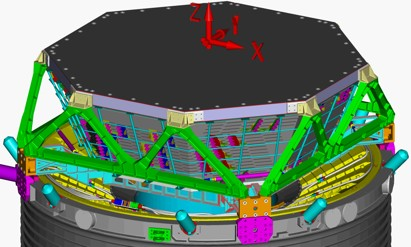
\includegraphics[height=0.35\paperheight]{TRD-Photo-05.jpeg}
	\end{center}
	\vspace{-0.45cm}
	\begin{block}{\small{The main features of TRD are:}}
		%\vspace{-0.25cm}
		\begin{itemize}\small{
			\item[$\circ$] \textbf{to discriminate} between  $e^+$ and $p$ whit a proton rejection of $10^{-2} \div 10^{-3}$ 
						in the energy range between $10$ and $300 GeV$.$^1$
						
			\item[$\circ$] \textbf{to identify} light nuclei by measurement of the charge $|Z|$.
		}\end{itemize}
%		\vspace{-0.55cm}
%		\begin{center}
%			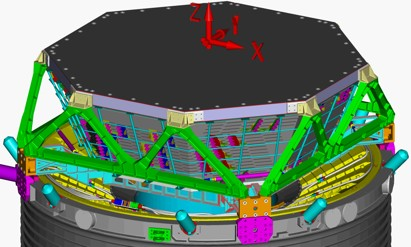
\includegraphics[height=0.35\paperheight]{TRD-Photo-05.jpeg}
%		\end{center}
	\end{block}
	\footnotetext[1]{\justifying
						This seems that, even if $e^+$ and $p$ 
						have the same charge, and so they are somewhat similar (i.e. in the other sub-detector, apart for the ECAL, 
						$e^+$ and $p$ with different energy give the same signals and therefore they may be confused), TRD may
						wrongly interpreter a $p$ as an $e^+$ only every $100 \div 1000$ real $p$ events.}
\end{frame}

\begin{frame}{TRD - Transition Radiation Detector}{the exploited physical process}
	\begin{columns}%[T]
	
		\begin{column}{0.5\textwidth}
			\justifying
			\small{The operating principle of TRD is mainly based on the known physical phenomenon, predicted by Ginzburg and 
			Frank in 1946 and observed, for the first time, by Goldsmith and Jelley in 1959, named:}
			
			\vspace{0.25cm}
			\begin{block}{Transition Radiation (TR)}
				\justifying
				TR is the electromagnetic radiation that is emitted whenever a charged particle transverse the interface 
				between two media with different refractive indexes.
			\end{block}
		\end{column}
		
		\begin{column}{0.5\textwidth}
			\begin{center}
%				\vspace{-0.75cm}				%		se l'allignamento delle colonne è impostato su [T]
				\vspace{-0.4cm} 				%		se l'allignamento delle colonne non è impostato su [T]
				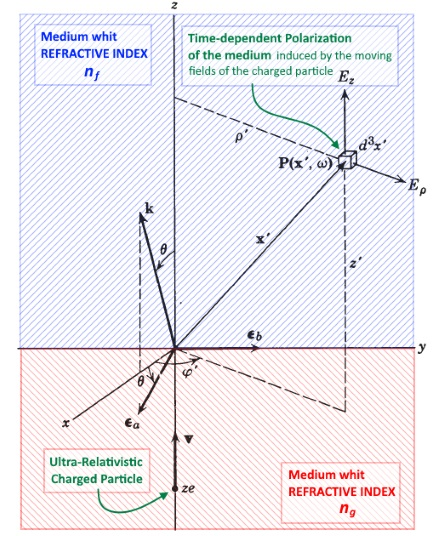
\includegraphics[width=0.9\columnwidth]{TransitionRadiation-ColorVers02mid.jpg}
			\end{center}
		\end{column}
		
	\end{columns}
\end{frame}

\begin{frame}[label=TRD-main]
	\frametitle{TRD - Transition Radiation Detector}
	\framesubtitle{the main features of transition radiation process}

	\small{
	Typically, this emission phenomena \textbf{is relevant for ultra-relativistic particles} ($\gamma \geqslant 300$) 
	and the emitted photon are \textbf{soft X-rays}, i.e. TR-photons have an energy of the order of a few $KeV$.
	
		\begin{itemize}
			\justifying
			\item  The \textbf{emission spectrum of  TR depends on} the density of the traversed material $\rho$, on the particle's energy $E$ and on the modulus of its electric charge $|Z|$.
%		ALTERNATIVA alla FRASE PRECEDENTE
%			\vspace{-0.1cm}
%			\begin{itemize} 
%				\item[$\circ$] density of the traversed material, $\rho$;
%				\item[$\circ$] energy of the particle, $E$;
%				\item[$\circ$] modulus of the electric charge of the particle, $|Z|$.
%			\end{itemize}					 % the density of the traversed material, on the particle's energy and on the modulus of its electric charge.
			\item \textbf{Total energy emitted per interface crossed, $W_{TR}$, is proportional to $\gamma$}.
			\item \textbf{Number of emitted TR-photons per interface crossed is small}, 
					 e.g. for a unit charge $N_{TR} \sim (3 \cdot 137)^{-1}$
			\item Exist a minimum distance $D_f$, called \textbf{formation zone}, that the particle has to traverse in order to efficiently emit TR photons.
			\item Due to the very small emission angle, $\theta_{TR} \lesssim \gamma^{-1}$, \textbf{TR-photons stay close to particle's track}.
		
		\end{itemize}
	}

	\vspace{-0.35cm}
	\hfill \hyperlink{TR-details}{\textbf{\beamerbutton{click here for more details on TR}}}
\end{frame}

\begin{frame}[label=TRD-Design]
	\frametitle{TRD - Transition Radiation Detector}
	\framesubtitle{based on a well-proven design}
	\small{
		\begin{columns}
			\begin{column}{0.675\textwidth}
				\justifying
				The \textbf{AMS-02  TRD is based on a well-proven design}\footnotemark[1] with multiple irregular boundary 
				crossings in a 20-mm fleece radiator and straw tube proportional wire chambers filled with 
				gas mixture ($80 \% \: \text{Xe} - 20\% \: \text{CO}_2$) to detect the TR-photons. 
			
				\vspace{0.15cm}
				The TRD consists of 20 layers of fleece and straw tube modules - in each layers there are several:
			\end{column}
			\begin{column}{0.325\textwidth}
				\vspace{-4ex}
				\begin{center}
					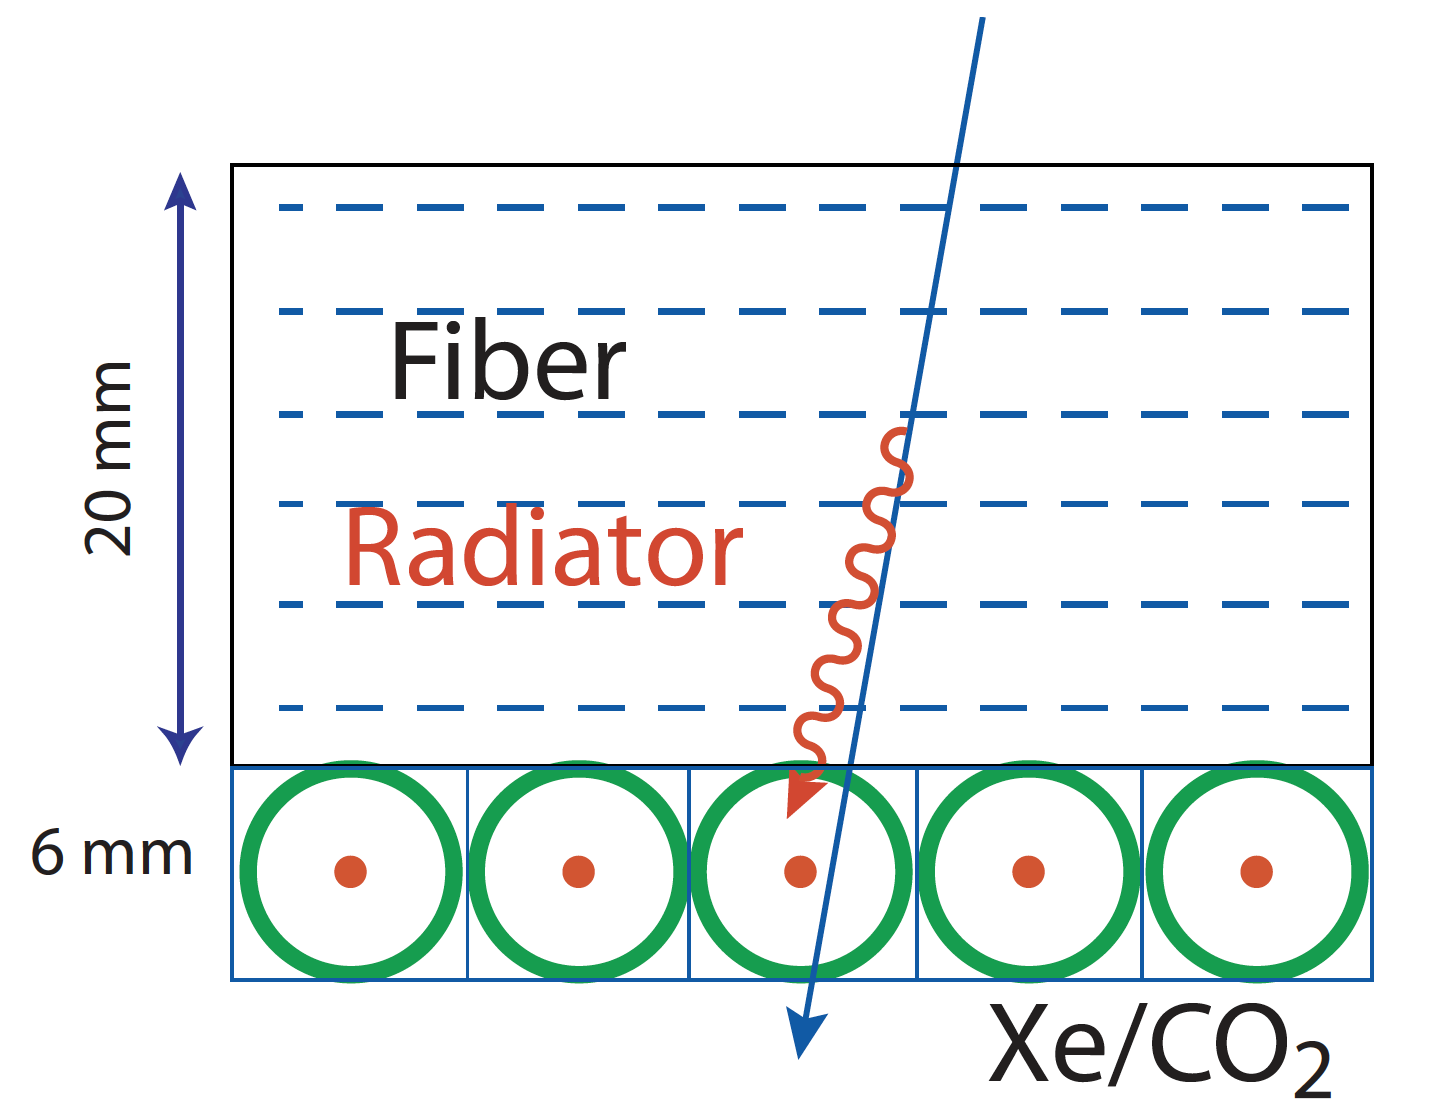
\includegraphics[width=\columnwidth]{TRD-Stack.png}
				
					\hspace{0.4cm}\hyperlink{TRD-Module}{\textbf{\beamerbutton{photo of a TRD module}}}
				\end{center}
			\end{column}
		\end{columns}	
	
		%\vspace{0.15cm}
		\begin{itemize}
			\justifying
			\item \bluetextbf{TRD radiator}\\
				The fleece material LRP 375 BK has a density of $0.06 g/cm^3$ and polypropylene/polyethylene 
				fibers with a thickness of $10 \mu m$.
			\item \bluetextbf{TRD straw modules}\\
				The TR-photons are detected in proportional mode modules, each consisting of 16 straw tubes.
		\end{itemize}
		\footnotetext[1]{This coming from the R\&D work for ground based experiments - ATLAS and HERA}
	}
\end{frame}


\begin{frame}[label=TRD-Straws]
	\frametitle{TRD - Transition Radiation Detector}
	\framesubtitle{more about the straw tubes of a TRD straw module}
	\justifying
	The straw tubes have a diameter of 6 mm and different lengths, up to 2m. Their walls, made of 72 $\mu m$ a 
	double-layer kapton–aluminum foil, work as cathodes. In the center of each tube, there is a 30 $\mu m$ thick fine 
	gold plated wire (tensioned with 1N) that works as anode for the proportional chamber.

	\vspace{-0.15cm}
	\begin{columns}
		\begin{column}{0.125\textwidth}\end{column}
		\begin{column}{0.75\textwidth}
			\begin{figure}
				\centering
				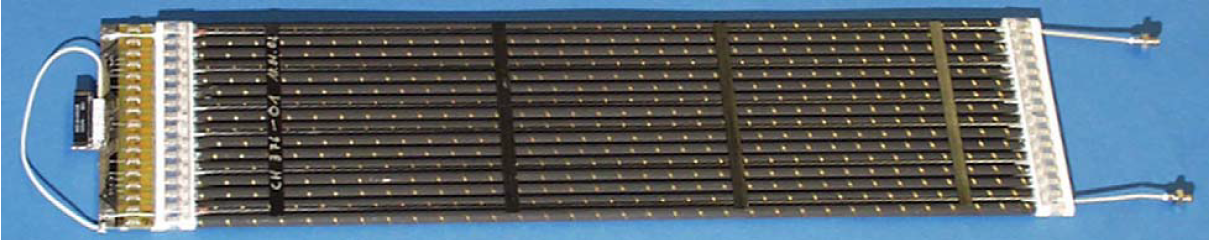
\includegraphics[width=\textwidth]{TRD-StrawMod-01.png}
				\vspace{0.1cm}
				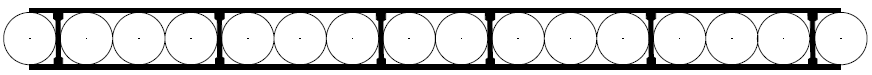
\includegraphics[width=0.75\textwidth]{TRD-StrawMod-02.png}
				\footnotesize{\caption{\justifying An example of a TRD straw module (up) and a schematic view of its section (down),
				 where also are drawn the longitudinal and vertical carbon fiber stiffeners used for the mechanical stabilization of the
				 module.}}
			\end{figure}
		\end{column}
		\begin{column}{0.125\textwidth}\end{column}
	\end{columns}
\end{frame}


\begin{frame}
	\frametitle{TRD - Transition Radiation Detector}
	\framesubtitle{the most critical design issue}
	\justifying
	\footnotesize{The most critical design issue is \textbf{the gas tightness of the straw modules}. In the vacuum of space,
	\textit{gas continuously diffuses out of the straw tubes}.  In order to operate the detector at stable parameters and to 
	compensate the gas gain change due to gas diffusion, a daily high voltage adjustment is performed, and the gas is refilled every 
	month by a gas supplier system.}

	\vspace{-0.65cm}
	\begin{columns}
		\begin{column}{0.1\textwidth}\end{column}
		\begin{column}{0.8\textwidth}
			\begin{figure}
				\centering				
				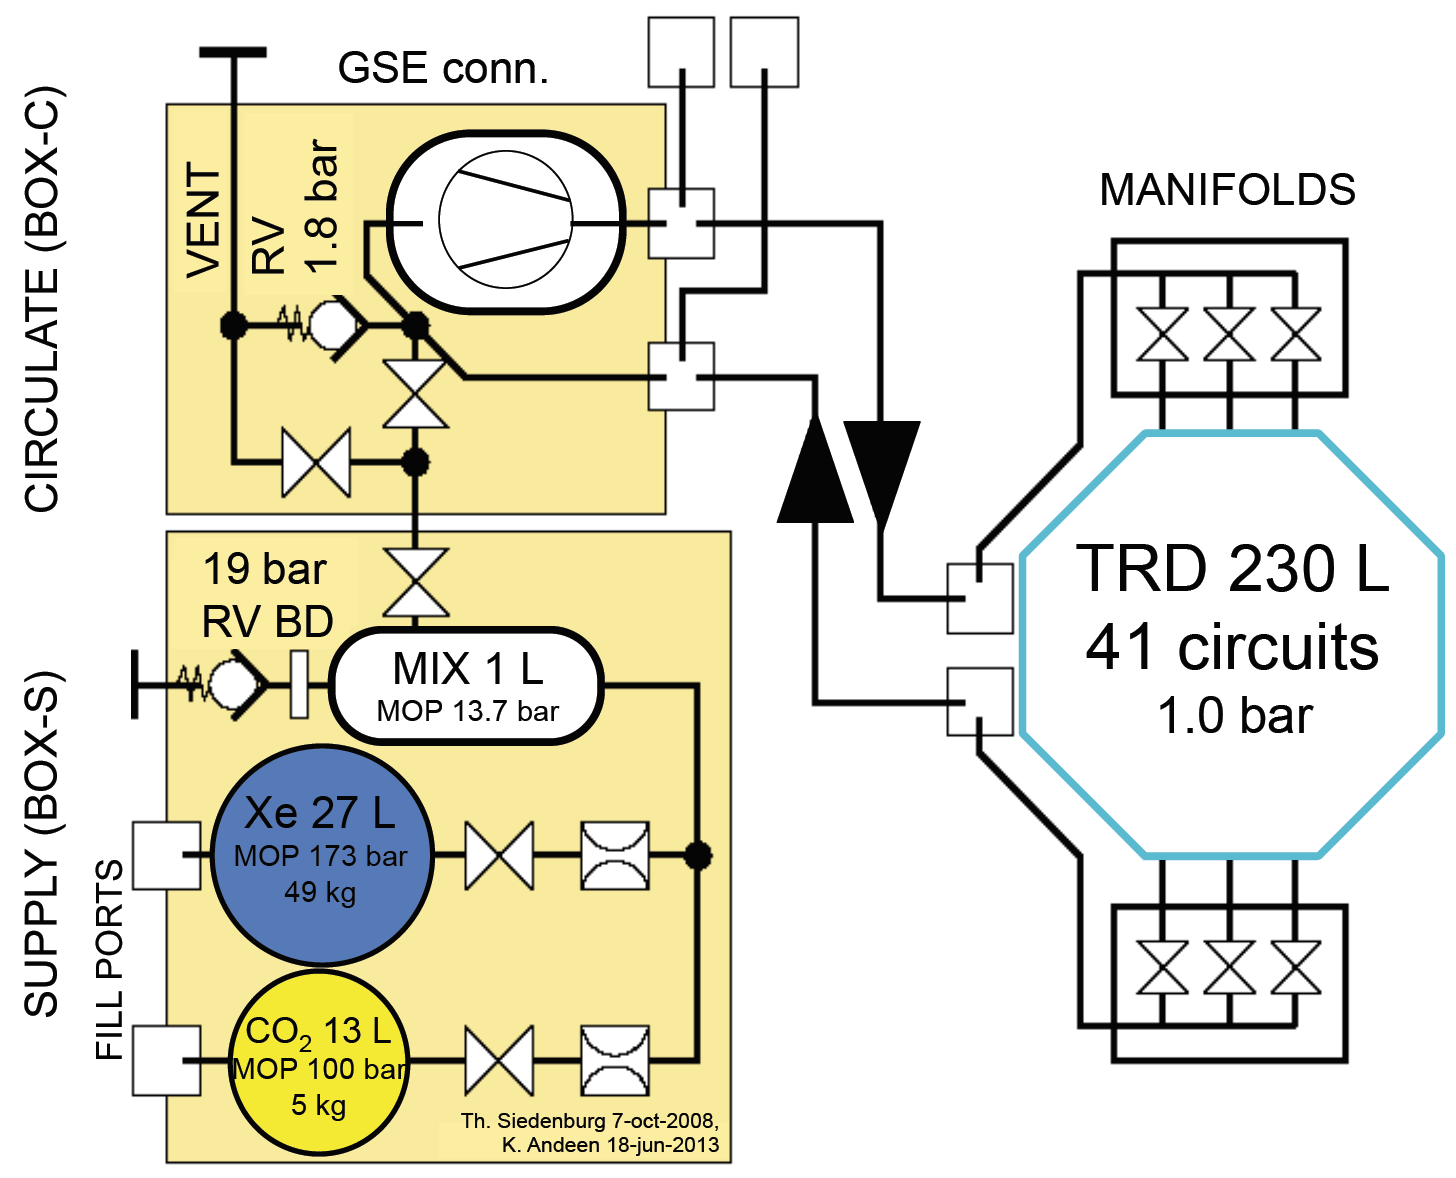
\includegraphics[height=0.35\paperheight]{TRD-GasSystem-05.png}
				\hfill
				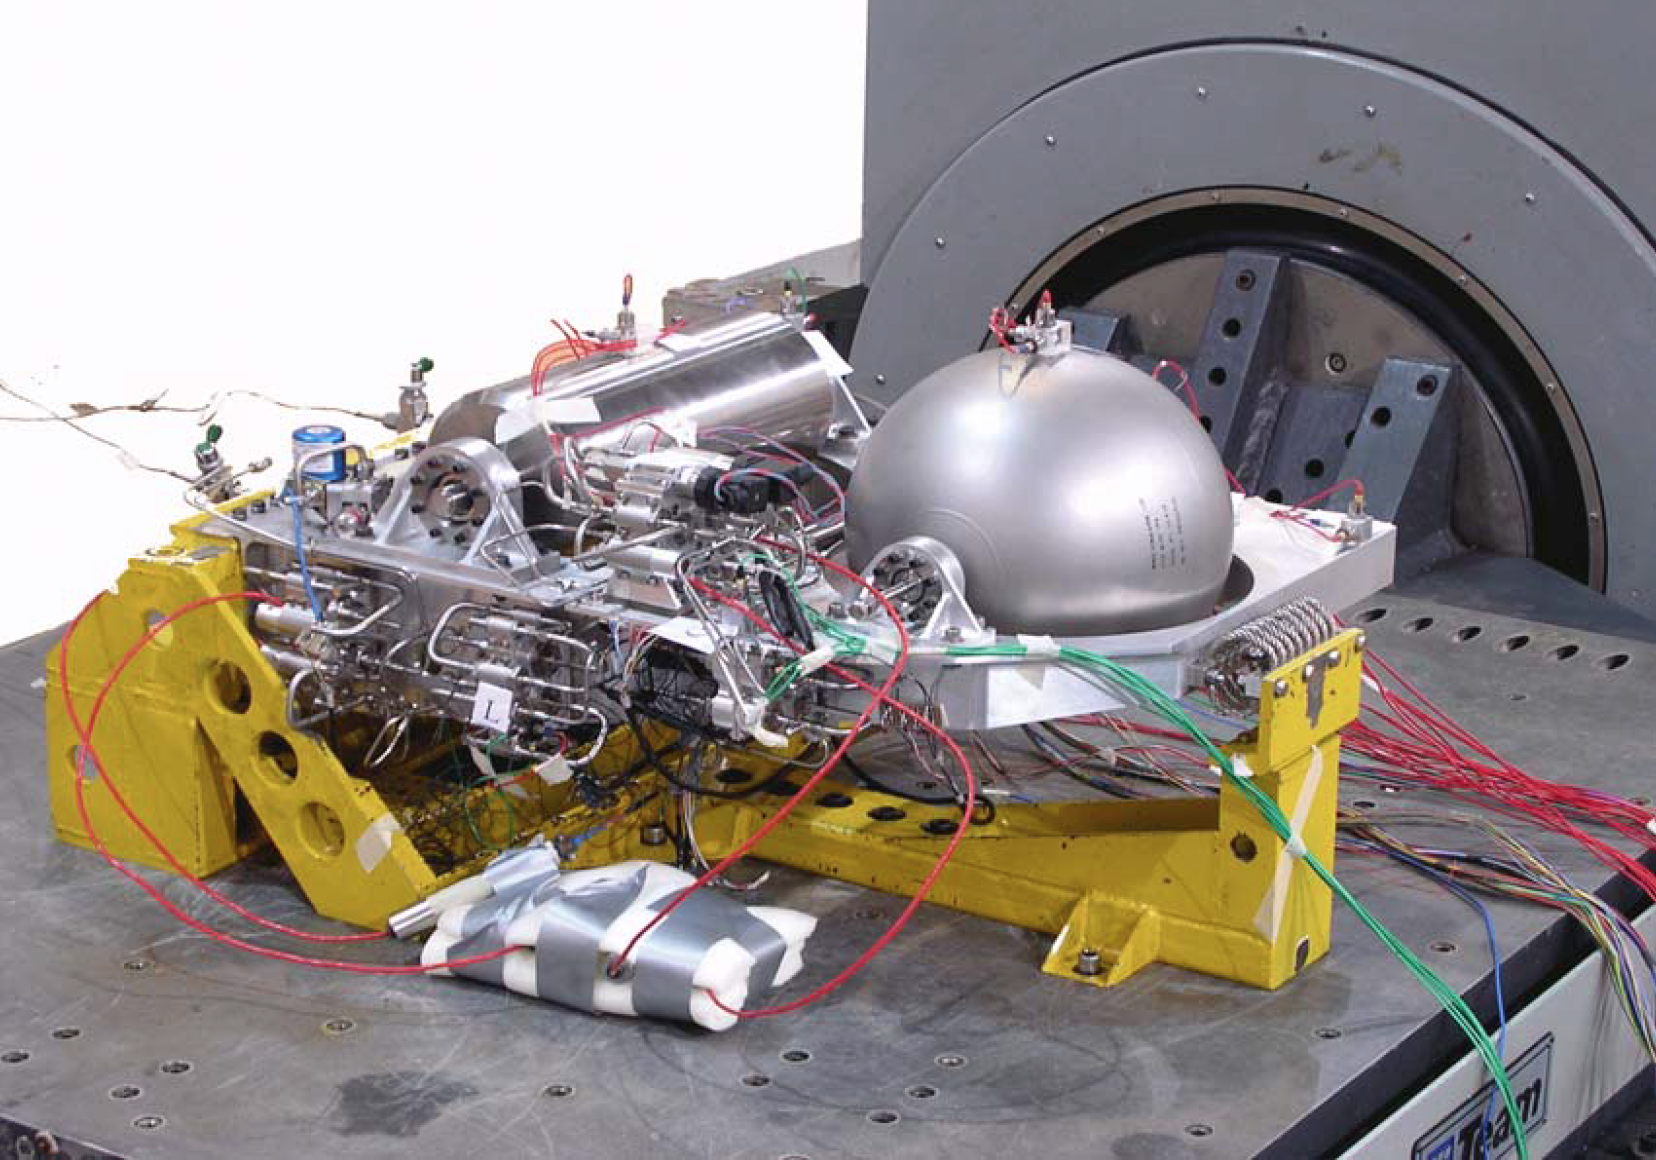
\includegraphics[height=0.35\paperheight]{TRD-GasSystem-01.png}
			\end{figure}
		\end{column}
		\begin{column}{0.1\textwidth}\end{column}
	\end{columns}	
	
	\vspace{0.15cm}
	\begin{columns}
		\begin{column}{0.05\textwidth}\end{column}
		\begin{column}{0.9\textwidth}
			\justifying
			\scriptsize{\textitem{Figure}{TRD gas system}: The gas in the supply boxes is first 
			mixed (BOX-S), visible in the photo. A pump (BOX-C) helps the circulation of the gas through 41 gas circuits, feeding the
			whole TRD detection volume. Each gas circuit is composed of eight straw tubes connected in series. Ten separate 
			manifolds with a shut-off valve control a variable number of gas circuits. Single gas groups can be isolated in case of a gas 
			leak in a tube.}
		\end{column}
		\begin{column}{0.05\textwidth}\end{column}
	\end{columns}
\end{frame}


\begin{frame}
	\frametitle{TRD - Transition Radiation Detector}
	\framesubtitle{gas system location}
	\justifying

	\begin{figure}
		\centering
		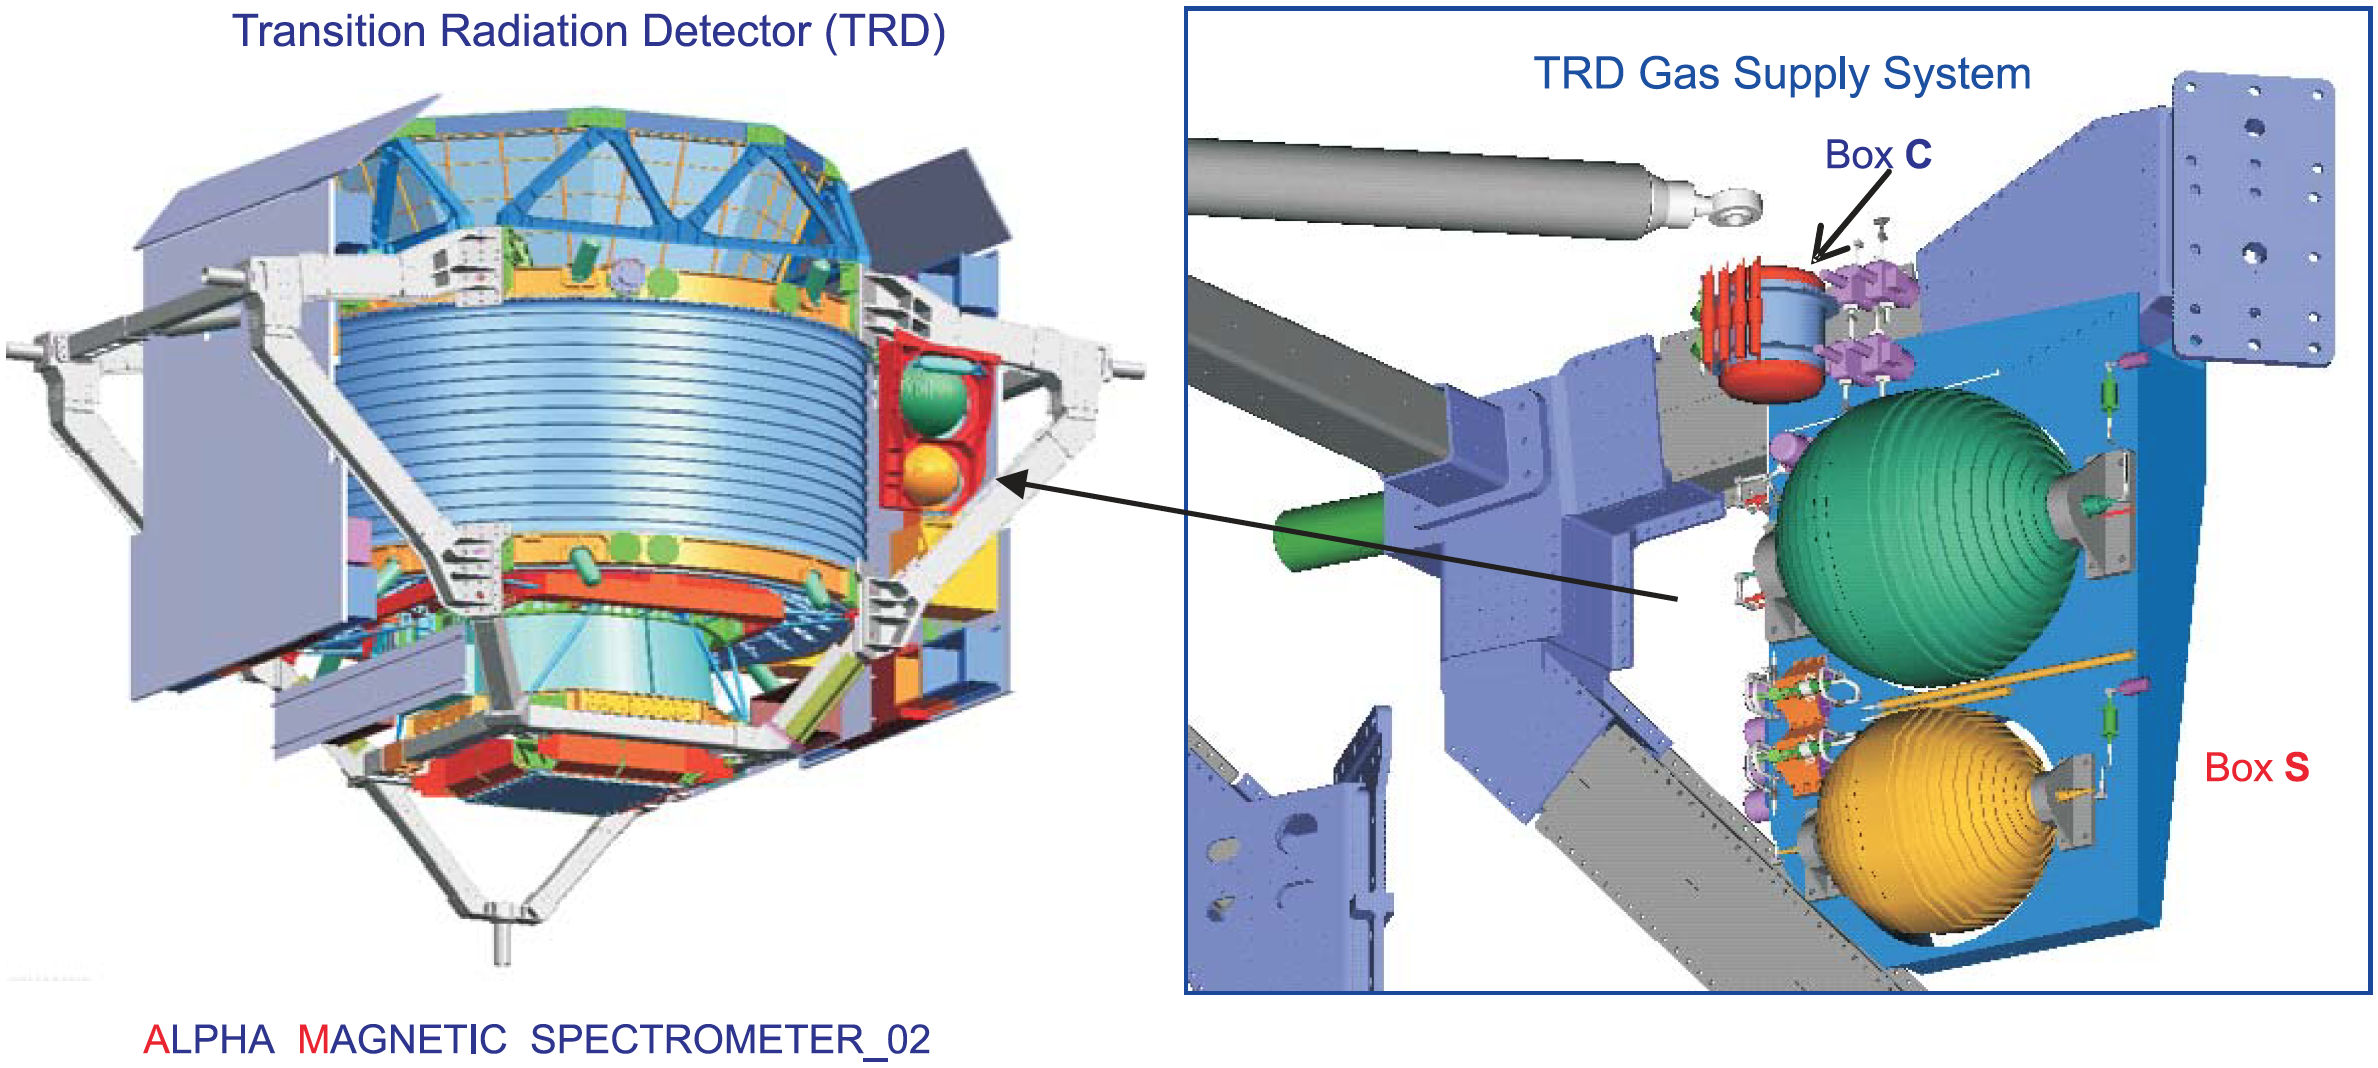
\includegraphics[height=0.45\paperheight]{TRD-GasSystem-06.png}
			\vspace{0.075cm}
			
			\footnotesize{\bluetextbf{Figure:} Location of TRD Gas system elements}
	\end{figure}

	\vspace{-0.25cm}
	\small{The available supplies of gas, $49.5 kg$ of Xe and $4.5 kg$ of $\text{CO}_2$, will have to last for three years of 
	operation. 
	Using as standard conditions $1 \, bar$ and 298 $^{\circ}{K}$, this corresponds to $8420 \, l$ of Xe and $2530 \, l$ 
	of $\text{CO}_2$.}
\end{frame}


\begin{frame}
	\frametitle{TRD - Transition Radiation Detector}
	\framesubtitle{safety factor}
	\justifying
	\footnotesize{Since $\text{CO}_2$ molecules are smaller than Xe molecules, they are the component leaking the most.}					
	\vspace{-0.25cm}
	\begin{columns}
		\begin{column}{0.004\textwidth} \end{column}
		\begin{column}{0.575\textwidth} 
		\justifying		
		\footnotesize{The total TRD $\text{CO}_2$ leak rate of $1.5 \cdot 10^{-2} l \, mbar/s$ would correspond 
		(at standard conditions) to a loss of $\text{CO}_2$ over 3 years of $287 \, l$ or a 
		``\textbf{safety factor}''\footnotemark[1] of 8.8 with respect to the $\text{CO}_2$ supply.			
		
		\textit{Fabricated TRD modules are accepted if they have with a $\text{CO}_2$ safety factor better than 4.} 
		This can only be assured by testing each of the 5248 straws individually before producing a module.
		
		As shown in the histogram, \textit{the safety factor averaged over all modules selected for flight is $7.9$}.
		\textbf{This allow up to 20 years of operation on the ISS}.}
		\end{column}
		\begin{column}{0.417\textwidth}
			\begin{figure}
				\centering
				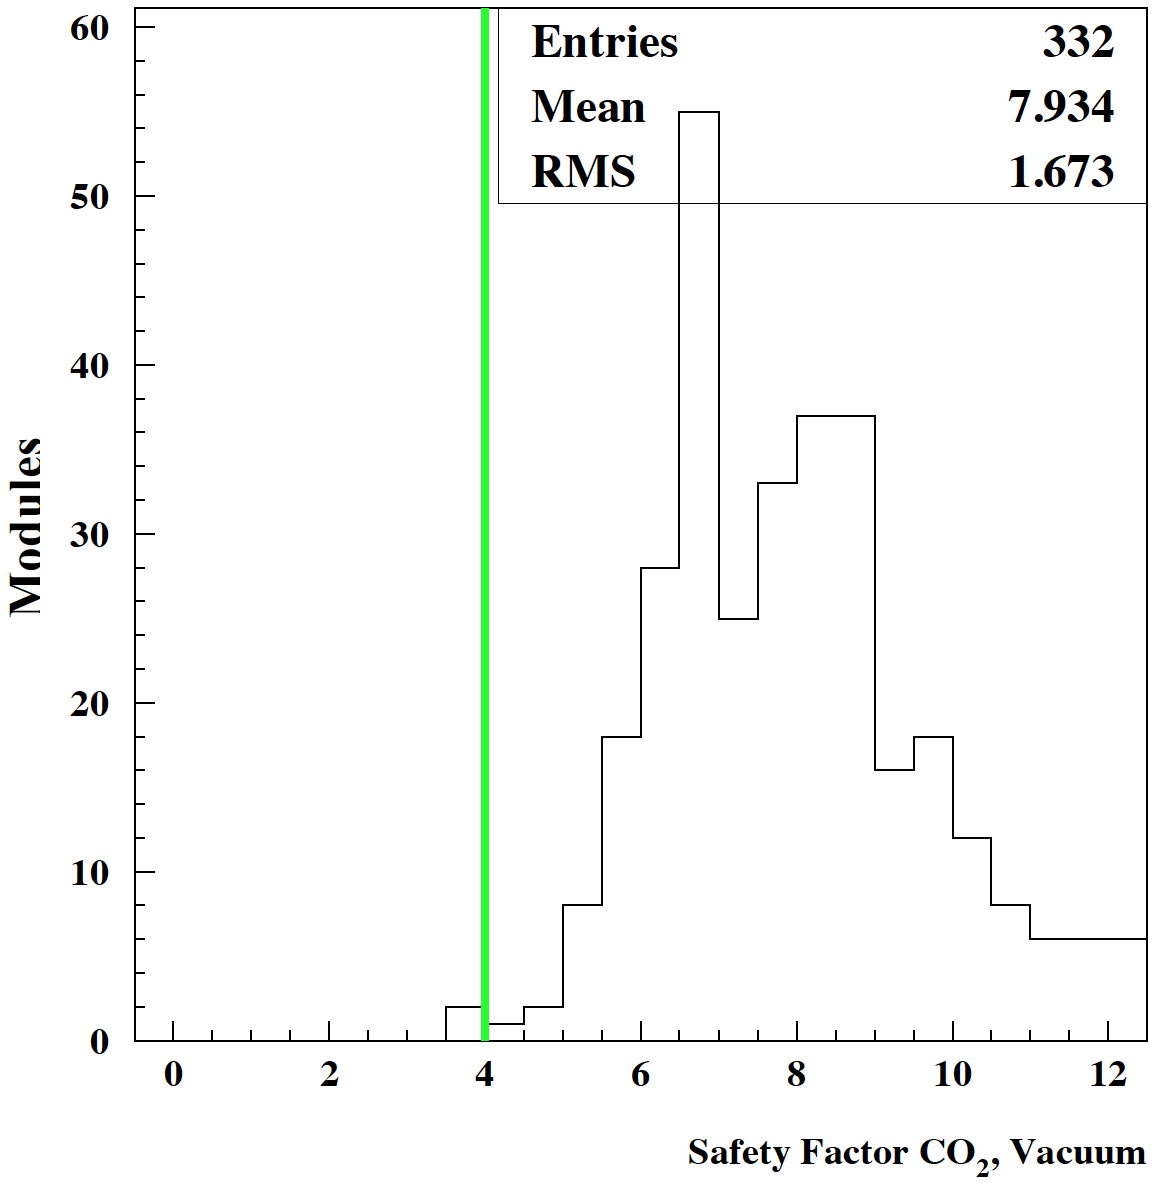
\includegraphics[width=0.975\columnwidth]{TRD-GasSystem-07.png}
				%\footnotesize{Straw module production: safety factor CO2}
			\end{figure}
		\end{column}
		\begin{column}{0.004\textwidth} \end{column}
	\end{columns}

	\footnotetext[1]{\justifying\scriptsize{Safety Factor (SF) describe the load carrying capacity of a system beyond the 
	expected or actual loads. In this case, it is the ratio between the volume of $\text{CO}_2$ stored, $2530 \, l$, and that lost 
	by diffusion in three years, $287 \, l$. Therefore, $\text{SF} = 2530 / 287 \simeq 8.8$.}}
\end{frame}


\begin{frame}[label=TRD-Supp_Struct]
	\frametitle{TRD - Transition Radiation Detector}
	\framesubtitle{the support structure of the TRD}%\hspace{2.2cm}\hyperlink{TRD-Mech_Struct}{\beamerbutton{more about 
%	the Mechanical Structure of the TRD}}}
	\justifying
	\small{In total, 328 modules (overall, 5248 straws) arranged on 20 layers that are supported by a conically shaped octagon
	structure made of aluminum honeycomb walls with carbon-fiber skins and bulkheads.}
	
	\vspace{-0.25cm}
	\begin{columns}
		\begin{column}{0.24\textwidth}\end{column}
		\begin{column}{0.37\textwidth}
			\begin{figure}
				\centering
				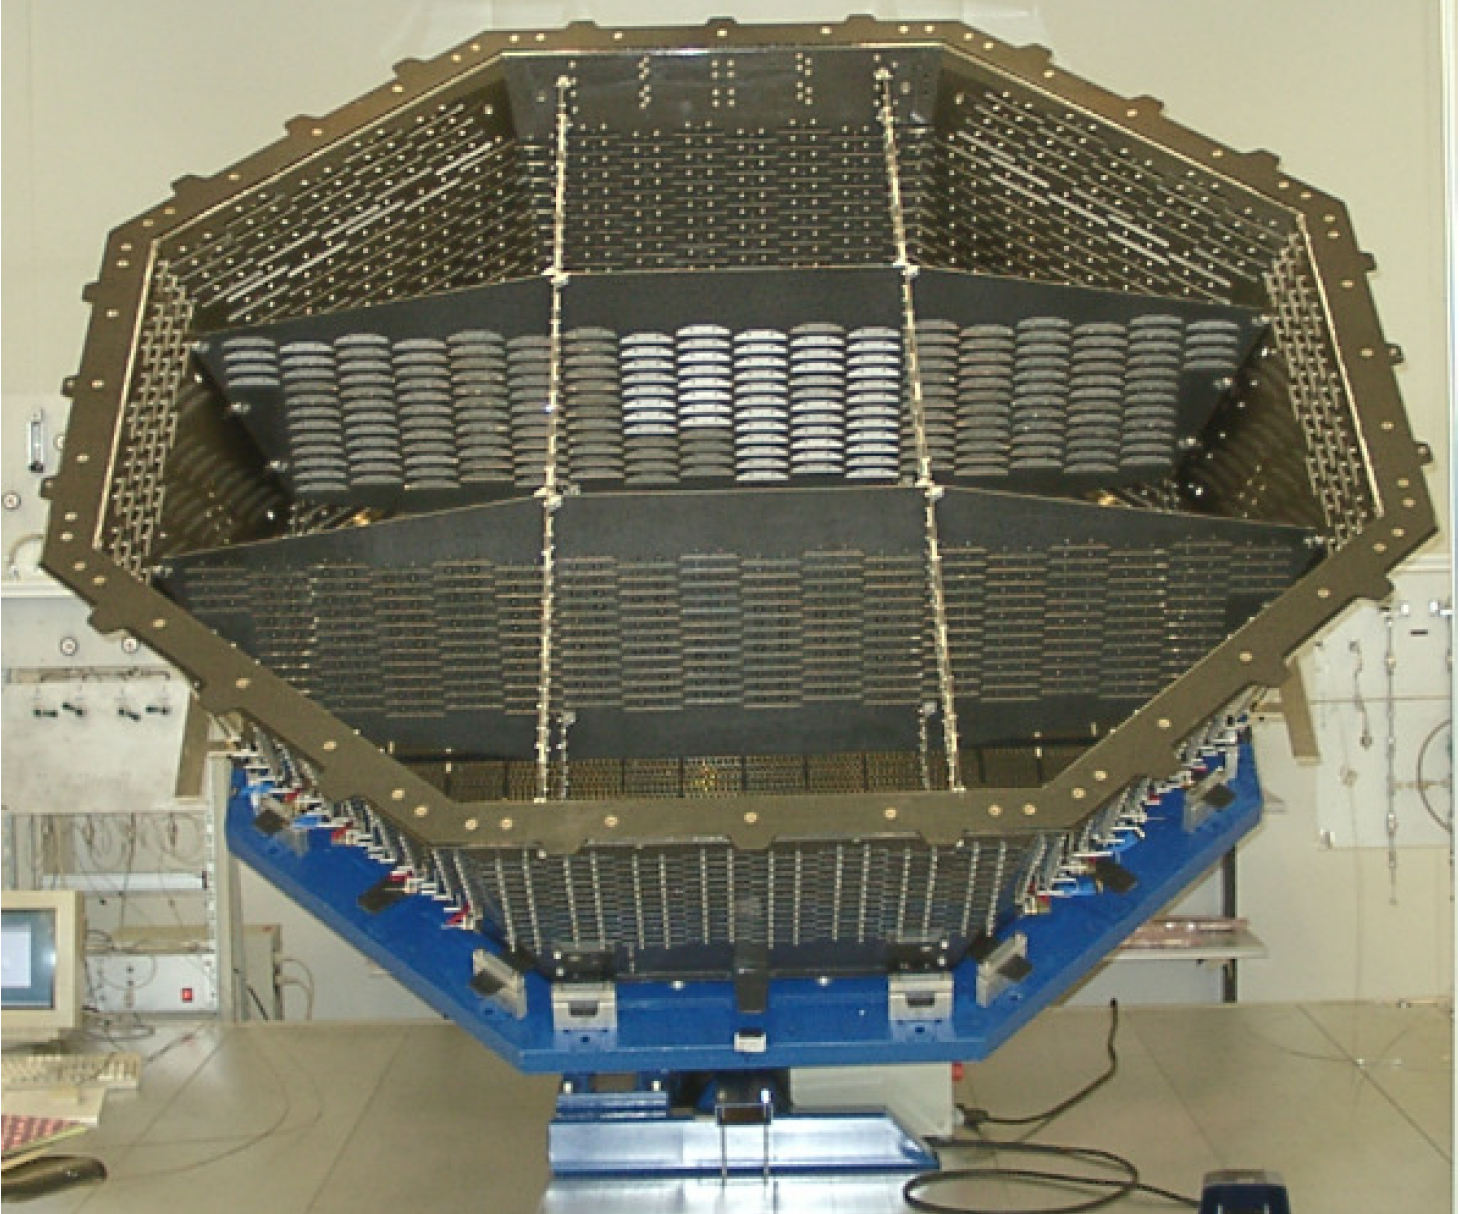
\includegraphics[width=\textwidth]{TRD-Support-05.png}
				
				%\footnotesize{\caption{\justifying AAA}}
			\end{figure}
		\end{column}
		\begin{column}{0.3\textwidth}\justifying
			
			\vspace{0.5cm}
			\footnotesize{\bluetextbf{Figure:}
			
			TRD support structure. 
			
			The \textbf{octagonal pyramid shape} has been chosen to optimize the TRD acceptance and to minimize the weight
			and the size of the apparatus.}
		\end{column}
		\begin{column}{0.09\textwidth}\end{column}
	\end{columns}
	
	\vspace{0.25cm}
	\small{The structure has a mechanical precision of 100 $\mu m$ to avoid wire displacement or straw walls deformation. 

	The upper and lower four layers run parallel to the magnetic field, the others perpendicular to \textbf{provide 3D 
	tracking}.}
%The TRD will be fully covered in a multi-layer-insulation (MLI) foil to keep the spatial orbit temperature gradient below 1K. 

	\vspace{-0.25cm}\hfill\hyperlink{TRD-Mech_Struct}{\beamerbutton{more on the TRD's Mechanical Structure}}
\end{frame}


\begin{frame}{TRD - Transition Radiation Detector}{the challenge for the AMS-02 experiment}
	\justifying
	\small{The challenge is to \textbf{build such a detector in a space-qualified way with strict limits} on outgassing, gas tightness, 
	weight and power consumption (less than $185 W$) whilst assuring safety and gas gain homogeneity in a harsh environment 
	during payload lift and in orbit without the possibility of further access to the experiment.}
	
	\vspace{-0.5cm}
	\begin{columns}
		\begin{column}{0.125\textwidth}\end{column}
		\begin{column}{0.65\textwidth}
			\begin{figure}
				\centering
				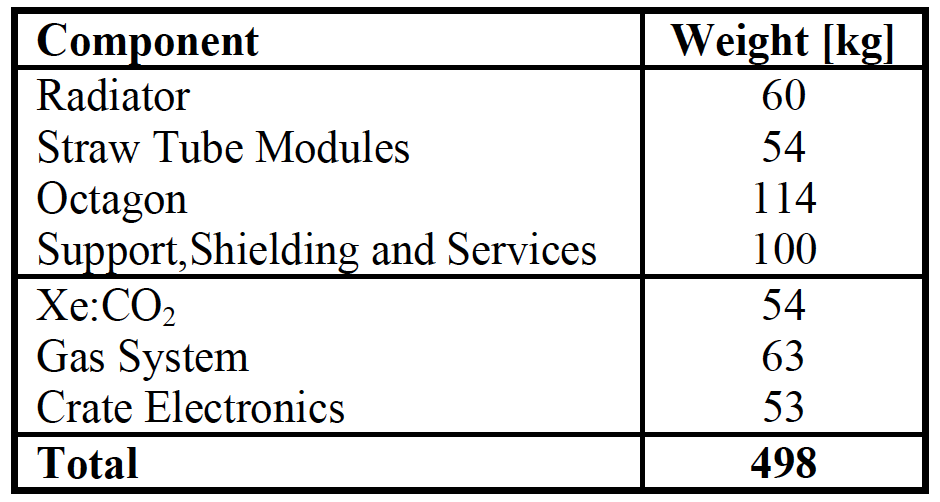
\includegraphics[width=0.75\textwidth]{TRD-Weights.png}
				
				\scriptsize{The optimized AMS-02 TRD design weighs less than $500 kg$.}
			\end{figure}
		\end{column}
		\begin{column}{0.125\textwidth}\end{column}
	\end{columns}
	
	\vspace{0.25cm}
	\small{This \textbf{involves} detailed \textit{finite-element calculations} as well as \textit{subcomponent vibration and 
	thermo-vacuum-cycle tests}.}
	
%	\footnotetext[1]{AMS-02 has a limited power consumption budget of $2000 W$, from which the TRD takes a part of less
%	than $185 W$.}	
\end{frame}

\begin{frame}[label=TRD-SQ_StrawsMod]
	\frametitle{TRD - Transition Radiation Detector}
	\framesubtitle{space qualification of the straw modules}
	\justifying	
	\small{Space qualification tests have been carried out for eight 0.7m long straw modules.}
	
	\vspace{-0.25cm}
	\begin{columns}
		\begin{column}{0.2\textwidth}\end{column}
		\begin{column}{0.45\textwidth}
			\begin{figure}
				\centering
				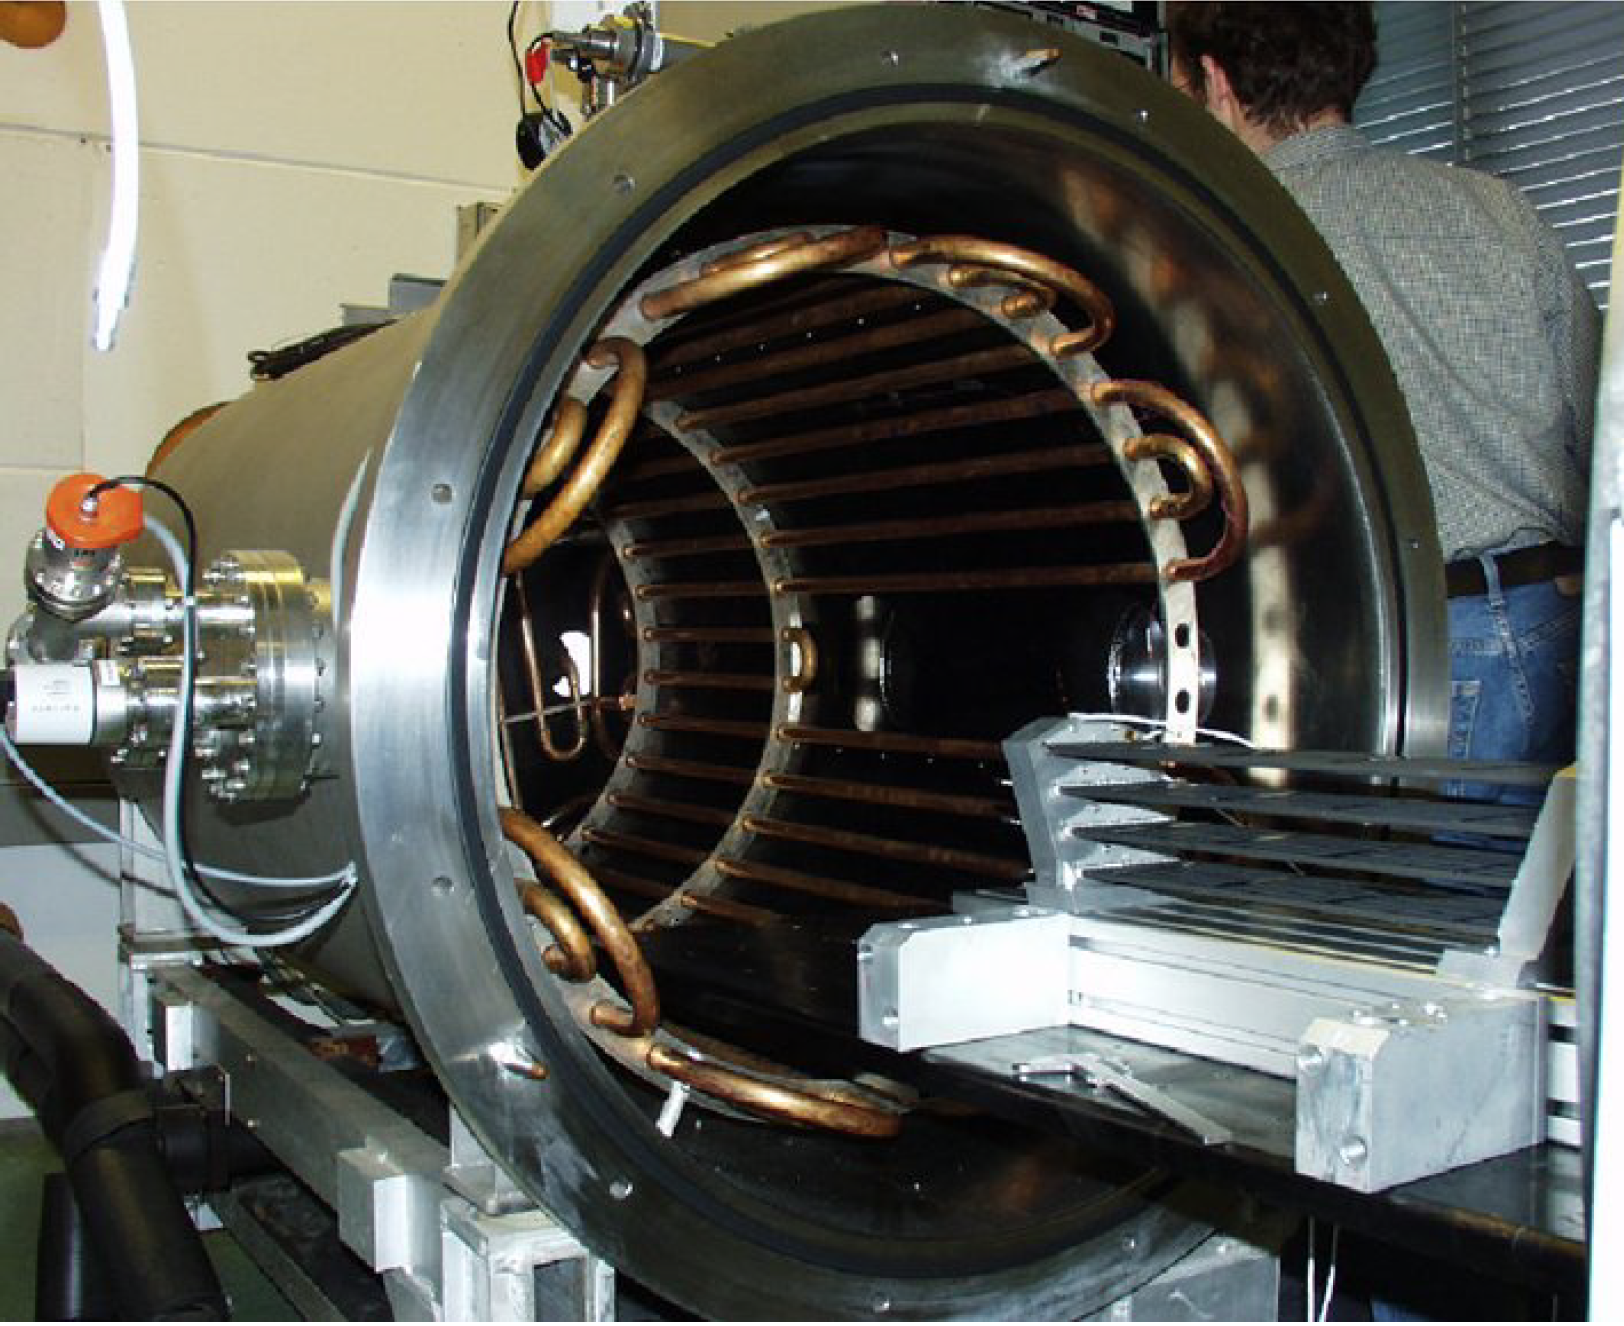
\includegraphics[width=0.95\textwidth]{TRD-StrawsQual-01.png}
				
				%\footnotesize{\caption{\justifying AAA}}
			\end{figure}
		\end{column}
		\begin{column}{0.27\textwidth}\justifying
			
			\vspace{0.5cm}
			\footnotesize{\bluetextbf{Figure}
			
			TRD thermal vacuum test of 4 straw detector modules}
		\end{column}
		\begin{column}{0.08\textwidth}\end{column}
	\end{columns}
	
	\vspace{0.25cm}
	\small{They underwent vibration tests (0.5 g sine sweep followed by 6.8 g random test followed by 0.5 g sine sweep) as
	well as thermo-vacuum-cycle tests (from -40 and +60 $^\circ{C}$) followed again by vibration tests. \textbf{No significant
	changes in eigenfrequencies, gas tightness or gas gain were observed.}}
	
	\hfill\hyperlink{TRD-SpaceQual}{\textbf{\beamerbutton{more details on Space Qualification}}}
\end{frame}

\begin{frame}
	\frametitle{TRD - Transition Radiation Detector}
	\framesubtitle{structural verification of the TRD support}
	\vspace{-1.15cm}
	\begin{columns}[t]
		\begin{column}{0.015\textwidth}\end{column}
		\begin{column}{0.425\textwidth}
			\begin{figure}
				\centering
				\small{\bluetextbf{Modal Analysis}}
				
				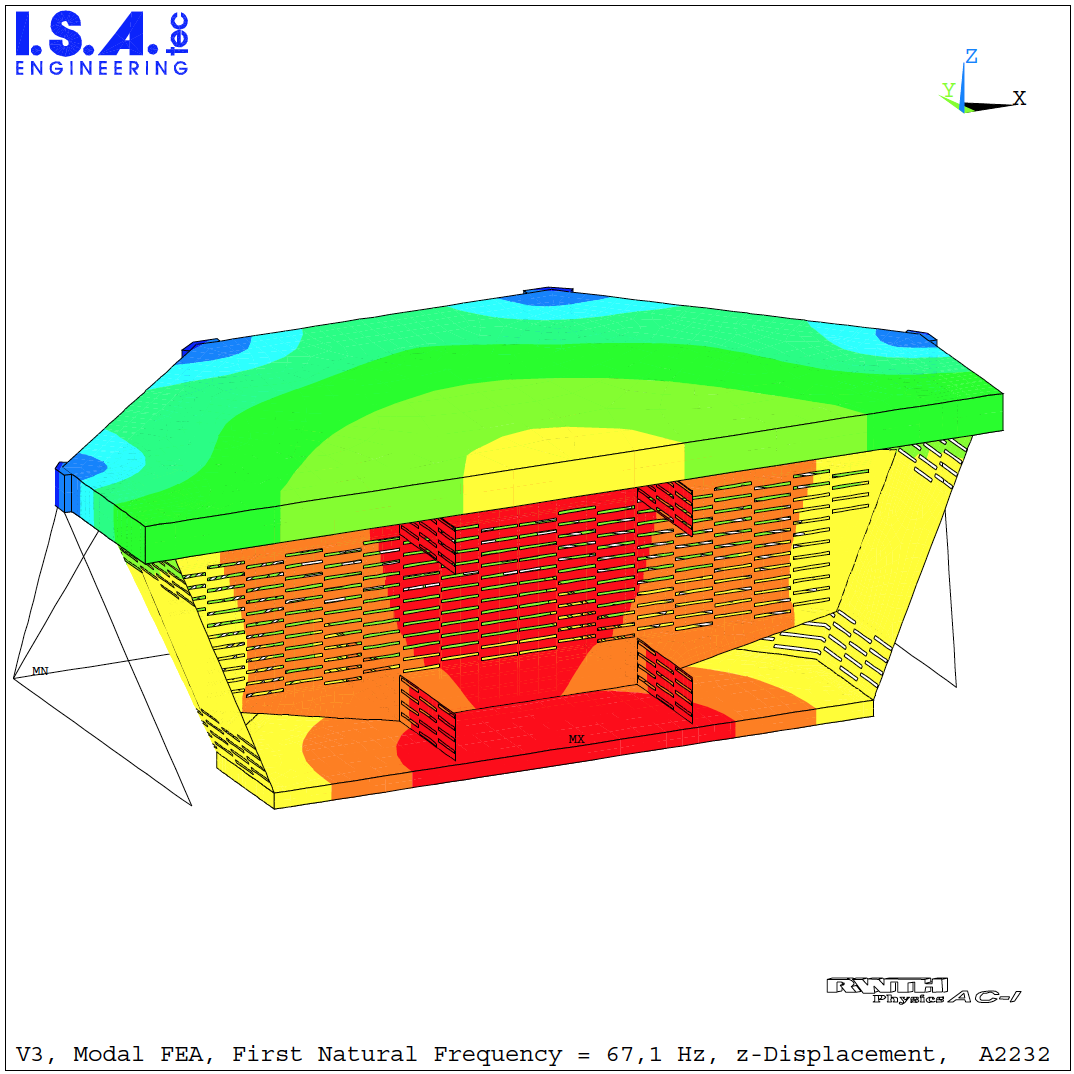
\includegraphics[width=0.725\textwidth]{TRD-Support-03.png}
				
				\justifying								
				\scriptsize{Finite-elements calculation \textbf{coupled load modal analysis}\footnotemark[1]:\\
								\hspace{0.17cm} - $f_0 = 67.1 Hz$\\
								\textbf{NASA requirement}: $f_0 > 50 Hz$}
			\end{figure}
		\end{column}
		\begin{column}{0.02\textwidth}\end{column}
		\begin{column}{0.425\textwidth}
			\begin{figure}
				\centering
				\small{\bluetextbf{Displacement}}
				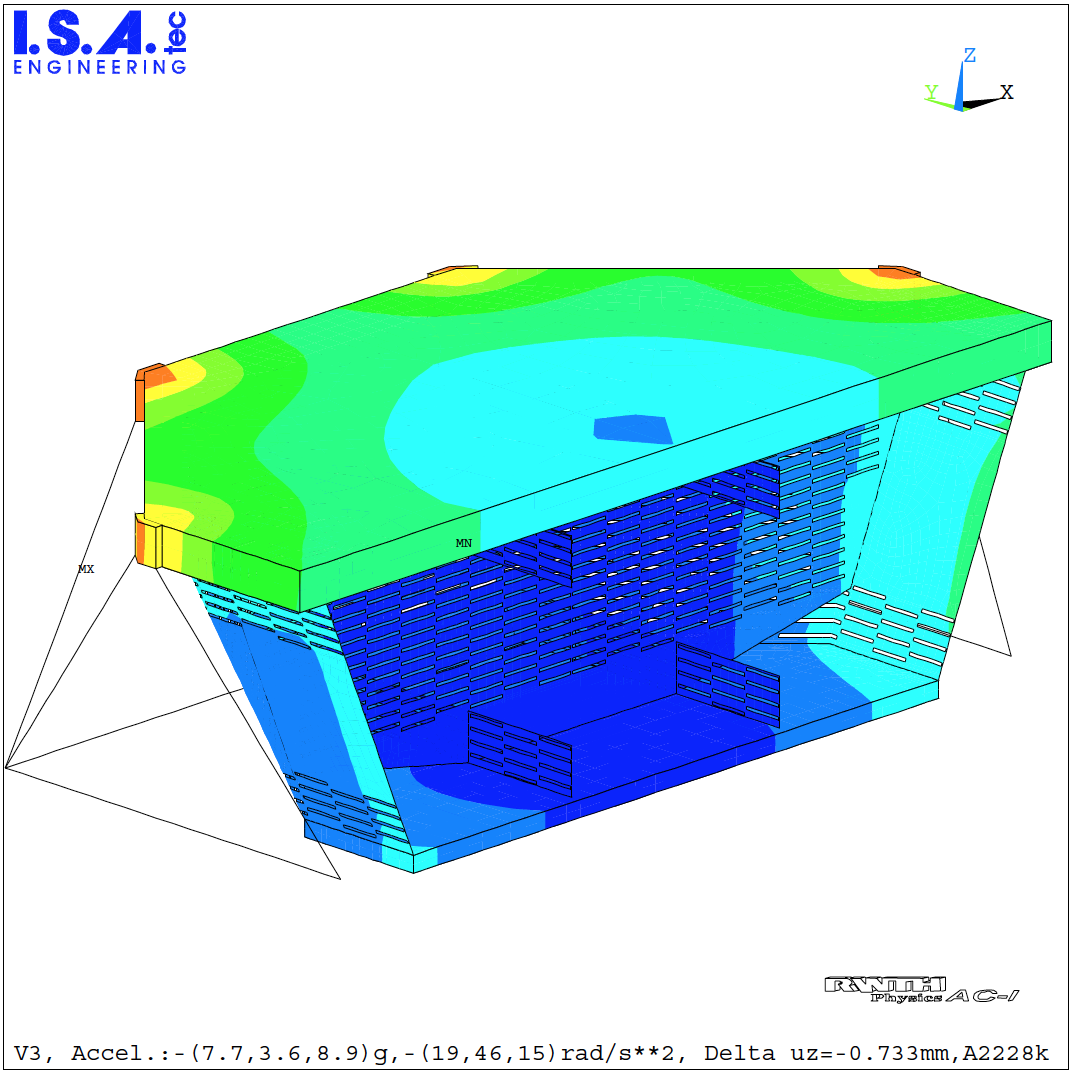
\includegraphics[width=0.725\textwidth]{TRD-Support-04.png}
				
				\justifying								
				\scriptsize{\textbf{Main accelerations} (simulating shuttle):\\
								\hspace{0.17cm} - $7.7g$ in $x$ at start; $8.9g$ in $z$ at landing.\\
								\textbf{Maximum displacement}:\\
								\hspace{0.17cm} - $0.73 mm$, well within elastic limits.}
			\end{figure}
		\end{column}
		\begin{column}{0.015\textwidth}\end{column}
	\end{columns}
	\footnotetext[1]{\justifying\scriptsize{
	Coupled loads modal analysis (CLA) is a critical process for many high-technology systems including launch vehicles and 
	satellites. CLA predicts responses caused by major dynamic and quasistatic loading events such as liftoff, gust, buffet, and 
	engine startup and shutdown.\\
	CLA helps to minimize risk and maximize the probability of mission success.}}
	
\end{frame}
%The TRD will be fully covered in a
%multi-layer-insulation (MLI) foil to keep the spatial orbit
%temperature gradient below 1K. 

%\begin{frame}
%	\frametitle{TRD - Transition Radiation Detector}
%	\framesubtitle{structural verification of the TRD gas system}
%	\justifying
%
%	\begin{figure}
%		\centering
%		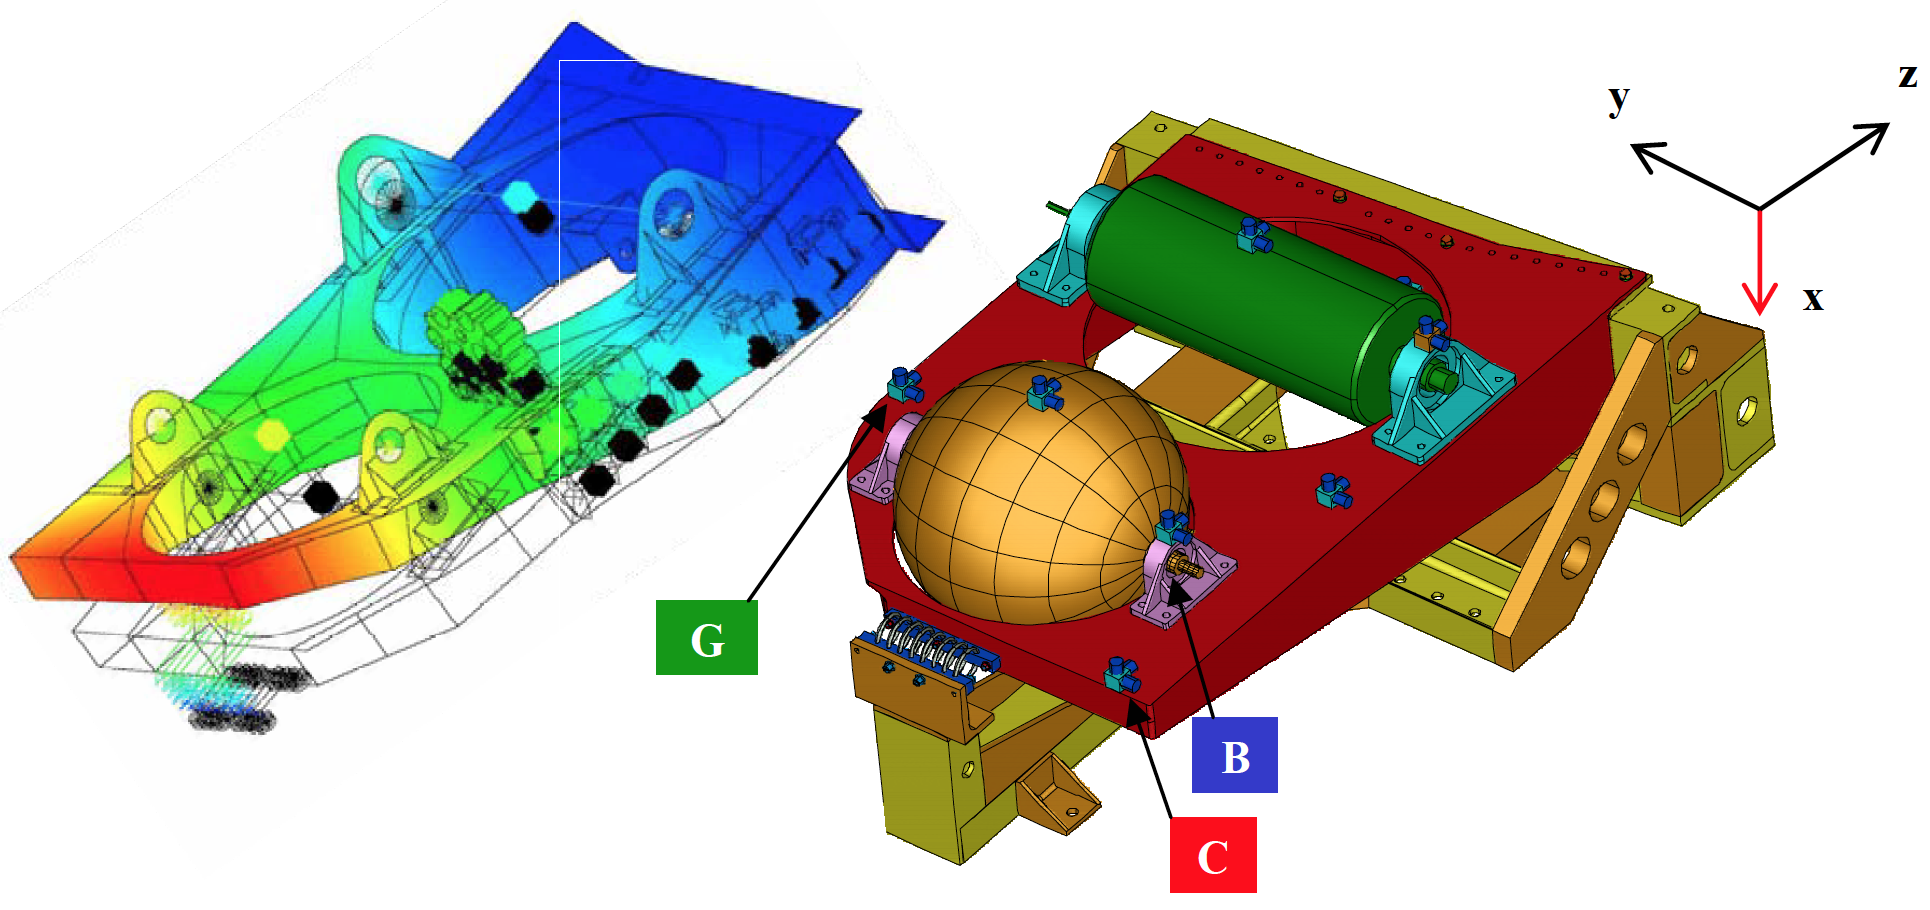
\includegraphics[height=0.45\paperheight]{TRD-GasSystem-08.png}
%			\vspace{0.075cm}
%			
%			\justifying
%			\footnotesize{\bluetextbf{Figure:} Vibration testing of the Box S mechanics. The figure in the left shows the results of FE modeling and the figure on the right the locations of the accelerometers during the test.}
%	\end{figure}
%\end{frame}

\begin{frame}
	\frametitle{TRD - Transition Radiation Detector}
	\framesubtitle{performance (proton rejection)}
	\justifying
	\small{The proton rejection power of the AMS-02 TRD design has been verified with a full 20 layer prototype in testbeams. 
	Protons are separated from electrons with a combined neural network analysis.
			 
	\vspace{-0.4cm}
	\begin{columns}
		\begin{column}{0.05\textwidth}\end{column}
		\begin{column}{0.45\textwidth}
			\begin{figure}
				\centering
				\hspace{0.5cm}\small{\bluetextbf{Tube-Energy Spectra}}
	
				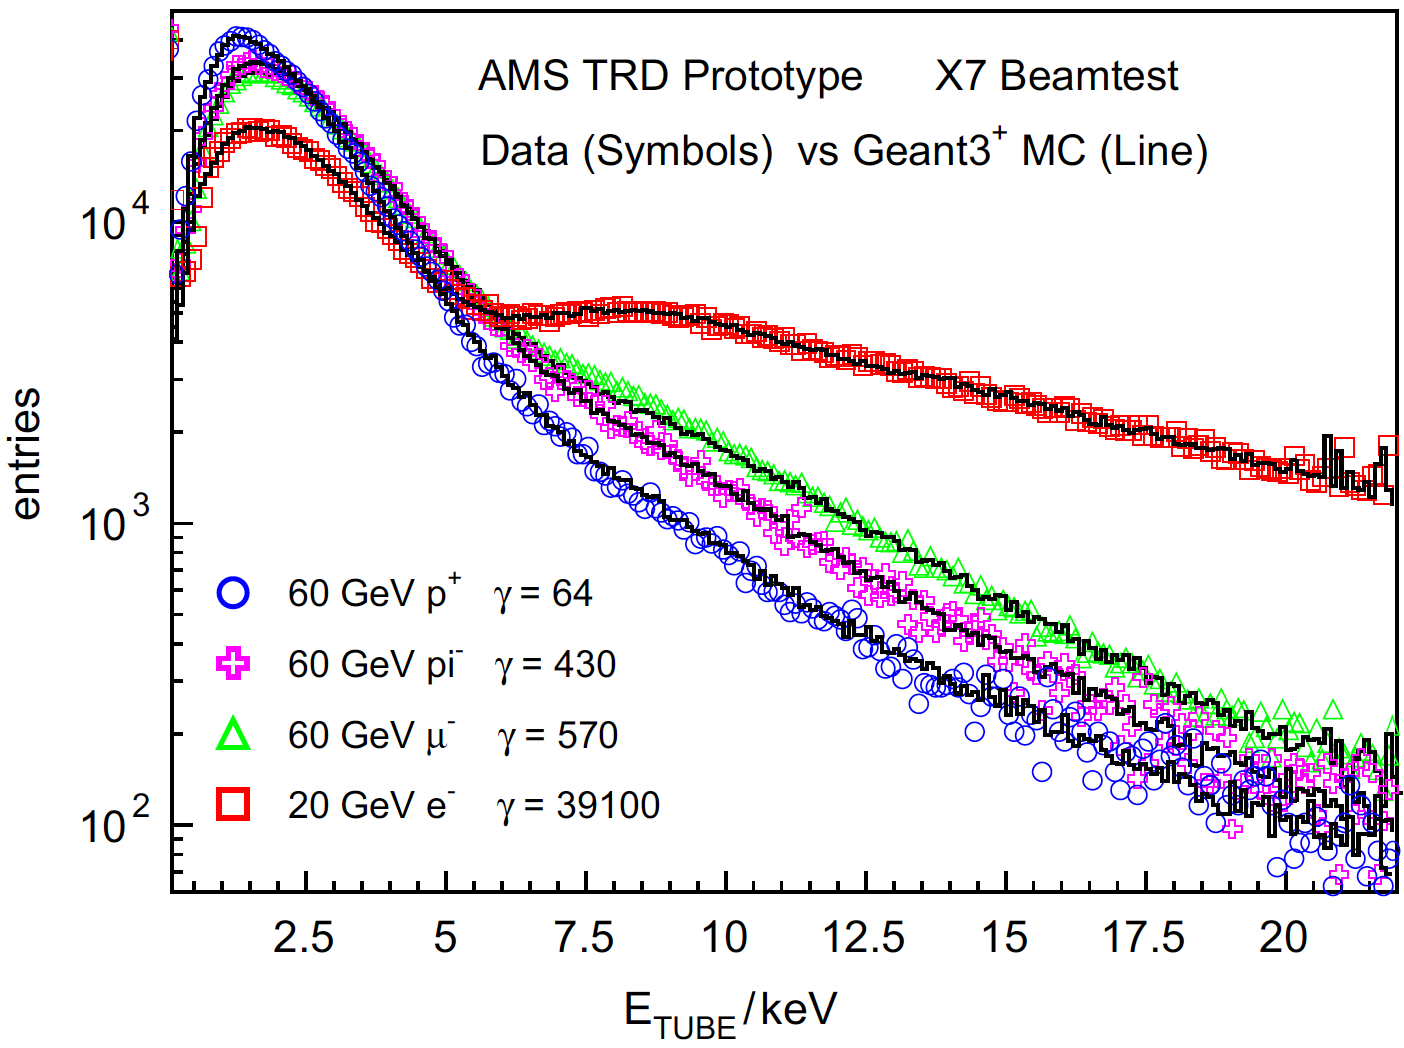
\includegraphics[height=0.35\paperheight]{TRD-TestBeam.png}
			\end{figure}
		\end{column}
		\begin{column}{0.45\textwidth}
			\begin{figure}
				\centering
				\hspace{0.5cm}\small{\bluetextbf{Proton Rejection}}
				
				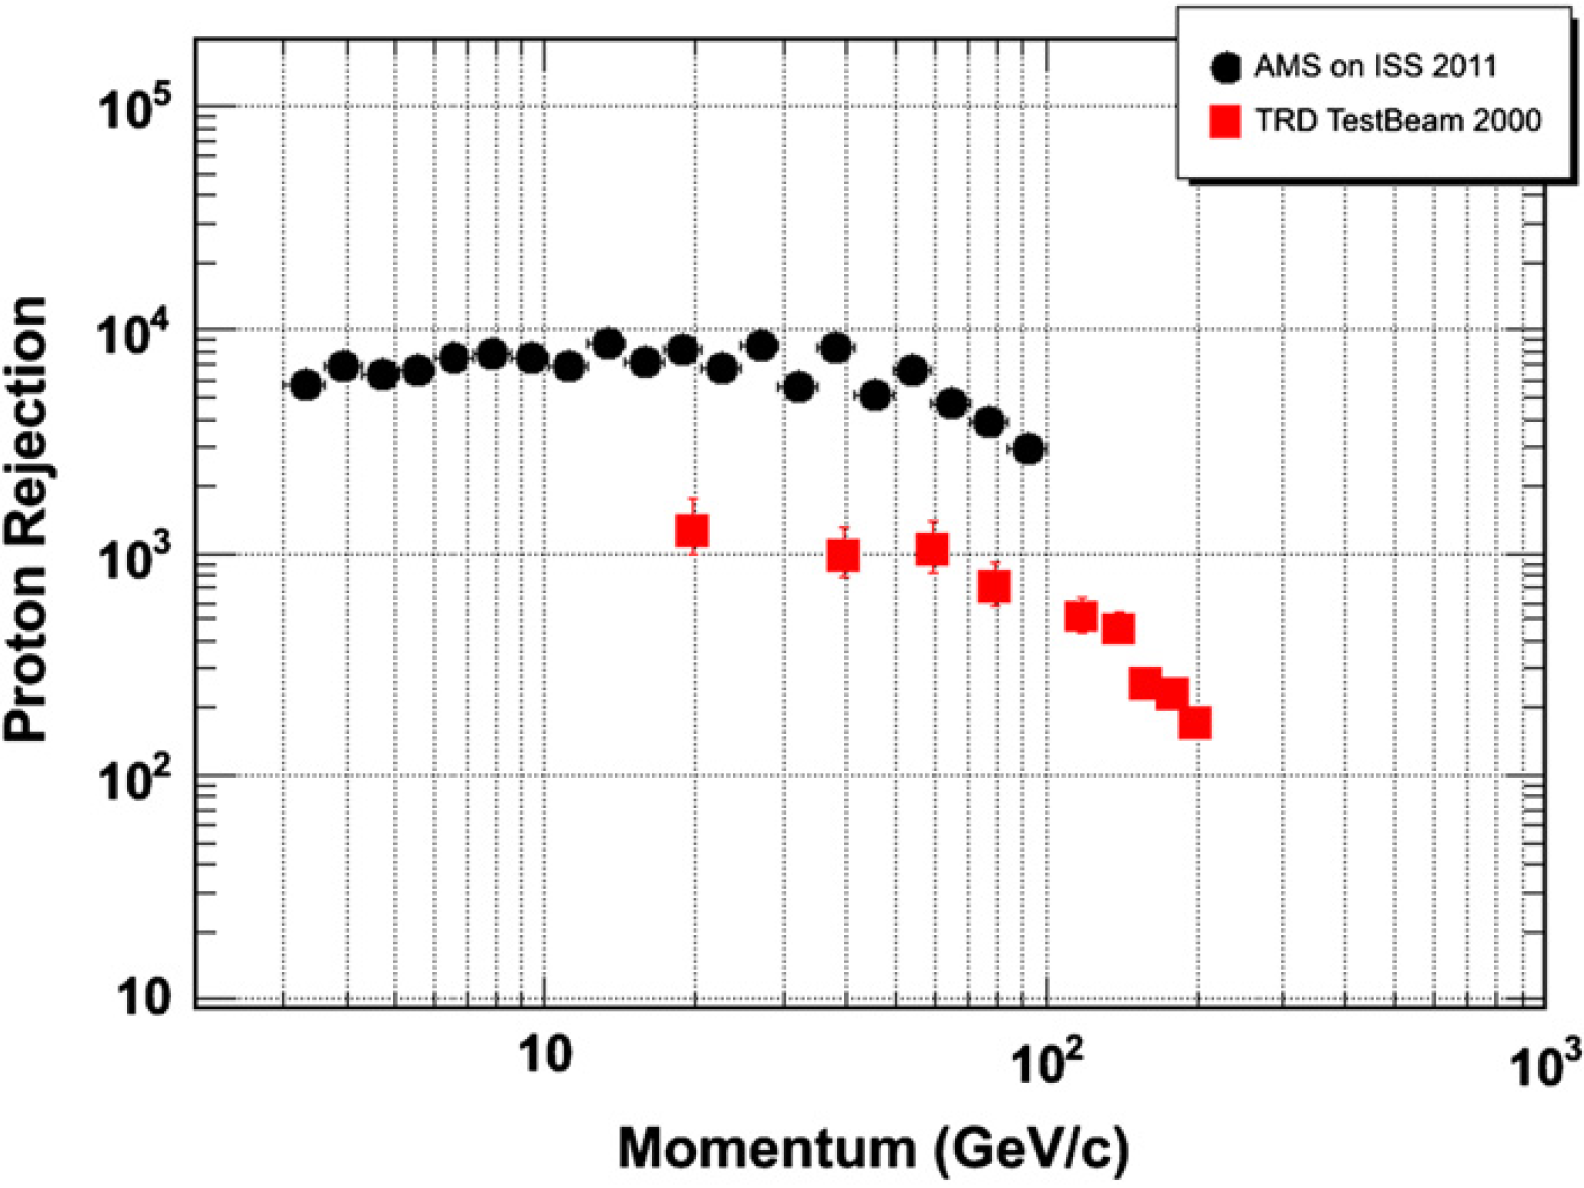
\includegraphics[height=0.35\paperheight]{TRD-ProtRej-03.png}
			\end{figure}
		\end{column}
		\begin{column}{0.05\textwidth}\end{column}
	\end{columns}
	
	\vspace{0.1cm}
	The \textbf{tube-energy spectra} are used as probability densities $\rho (E)$. 
	
	The \textbf{proton rejection}\footnotemark[1] is well above 100 at an electron efficiency of 90\% for proton beam energies between 15 and 250 $GeV$.}
	
	\footnotetext[1]{\justifying\scriptsize{TRD performs better in space than expected by rejection studies in beam tests on ground.}}
\end{frame}

\begin{frame}[label=TRD-ChargePerform1]
	\frametitle{TRD - Transition Radiation Detector}
	\framesubtitle{performance (measurement of the charge)}
	\justifying
	\vspace{-0.1cm}
	
	\small{To perform charge measurements is used the dependence of $dE/dx$ on particle charge, $Z$, that is also 
			dependent on path length and rigidity. }
		
	\vspace{-0.05cm}
	\begin{columns}
		\begin{column}{0.01\textwidth}\end{column}
		\begin{column}{0.5\textwidth}
			\justifying
			
			\small{Therefore, in AMS data analysis, \textbf{the distributions of $dE/dx$ in each tube} is parametrized as analytical 
			functions of these variables, called $dE/dx$ \textit{Probability Density Functions} ($dE/dx$ \textit{PDFs}), which are 
			used in determination of $Z$ by a likelihood method.

			\vspace{0.1cm}
			\textbf{For particles with $Z$ larger than 6, the ADC readout of the straw tubes is saturated}. }
			
			\vspace{0.1cm}
			To extend the measurements to 	particles with higher charge, as well as increase the			
		\end{column}
		\begin{column}{0.01\textwidth}\end{column}
		\begin{column}{0.47\textwidth}
			\centering
			\vspace{0.05cm}
			
			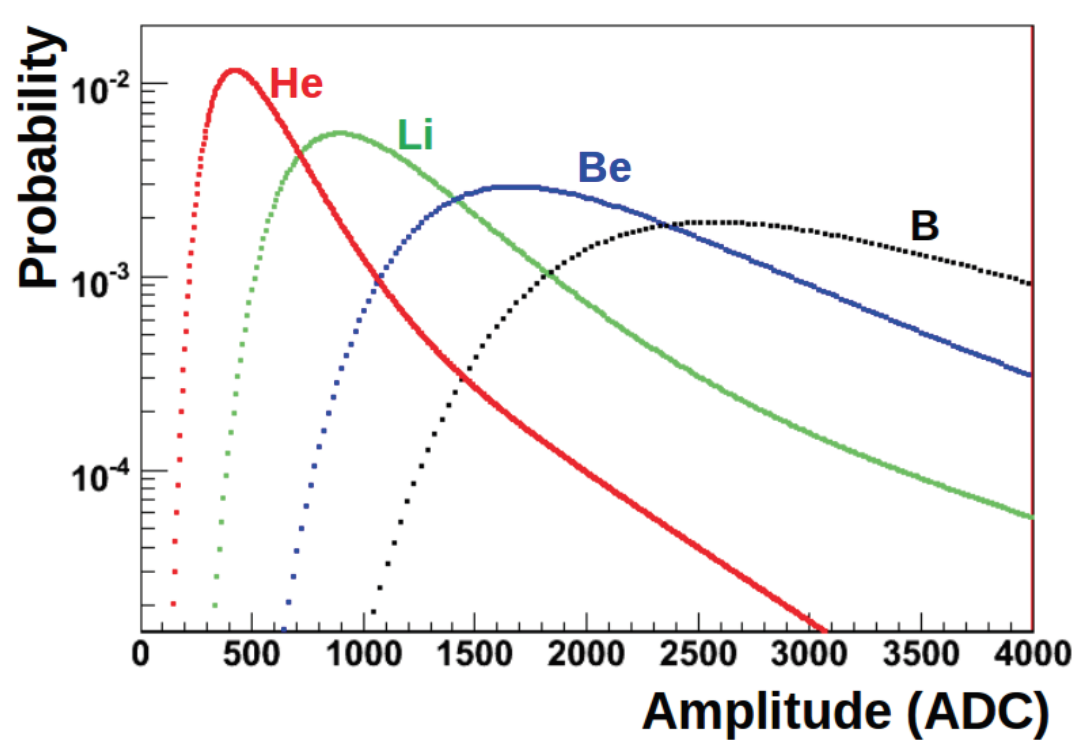
\includegraphics[width=\columnwidth]{TRD-ChargeMeas-dEPDFs.png}

			\vspace{-0.1cm}
			\begin{columns}
				\begin{column}{0.15\textwidth}\end{column}
				\begin{column}{0.8\textwidth}
					\justifying			
					\scriptsize{\bluetextbf{Figure:}\\
					$dE/dx$ \textit{PDFs} of He, Li, Be, and B, derived from flight data.}		
					%\vspace{0.1cm}
				\end{column}
				\begin{column}{0.05\textwidth}\end{column}
			\end{columns}						
		\end{column}
		\begin{column}{0.01\textwidth}\end{column}
	\end{columns}		
	
	\vspace{0.1cm}
	\small{resolution for light ions, additional information of the produced delta rays can also is utilized for charge measurements.}
	
	\vspace{-0.2cm}
	\hfill\hyperlink{TRD-DeltaTech1}{\textbf{\beamerbutton{more about delta rays technique}}}
\end{frame}

%% VERSIONE ALTERNATIVA DELLA SLIDE PRECEDENTE
%\begin{frame}
%	\frametitle{TRD - Transition Radiation Detector}
%	\framesubtitle{performance (measurement of the charge)}
%	\justifying
%	\vspace{-0.1cm}
%	\small{
%	To perform charge measurements is used the dependence of $dE/dx$ on particle charge, $Z$, that is also dependent on path 
%	length and rigidity. Therefore, in AMS data analysis, \textbf{the distributions of $dE/dx$ in each tube} is parametrized as analytical 
%	functions of these variables, called $dE/dx$ \textit{Probability Density Functions} ($dE/dx$ \textit{PDFs}), which are used in 
%	determination of $Z$ by a likelihood method.
%	
%	\vspace{-0.35cm}
%	\begin{columns}
%		\begin{column}{0.24\textwidth}\end{column}
%		\begin{column}{0.415\textwidth}
%			\begin{figure}
%				\centering
%				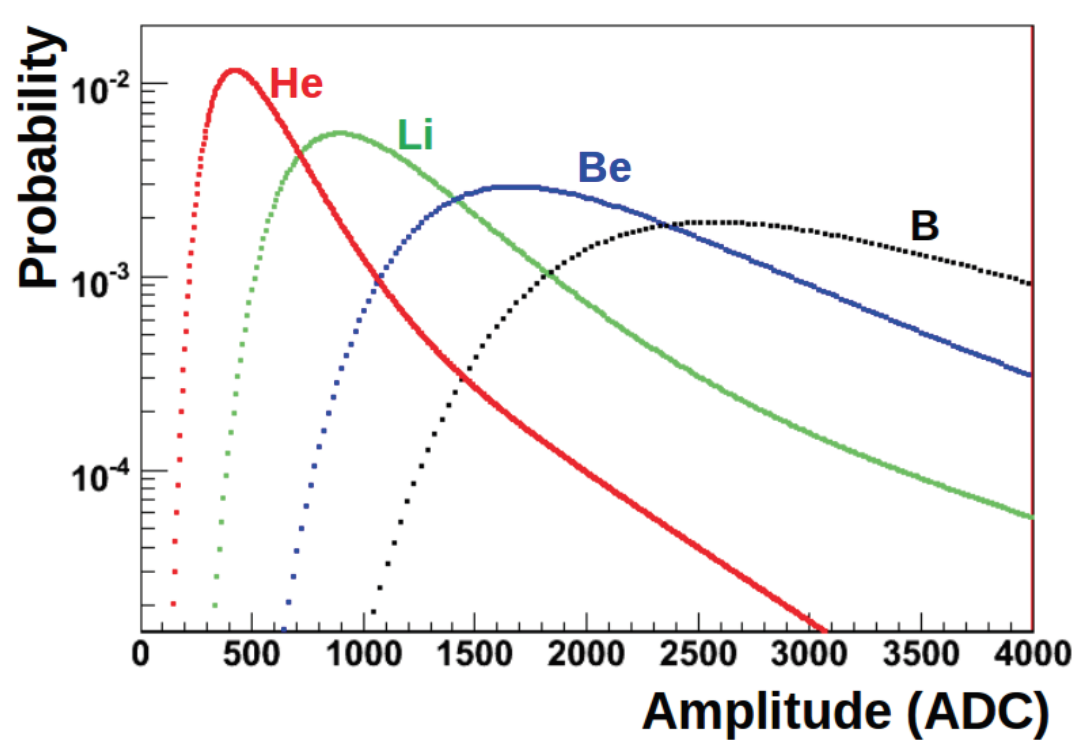
\includegraphics[width=0.95\textwidth]{TRD-ChargeMeas-dEPDFs.png}
%				
%				%\footnotesize{\caption{\justifying AAA}}
%			\end{figure}
%		\end{column}
%		\begin{column}{0.295\textwidth}\justifying
%			
%			\vspace{0.1cm}
%			\footnotesize{\bluetextbf{Figure}
%			
%			$dE/dx$ \textit{PDFs} of Helium, Lithium, Beryllium, and Boron, derived from flight data.}
%		\end{column}
%		\begin{column}{0.14\textwidth}\end{column}
%	\end{columns}
%	
%	\vspace{0.1cm}
%	\textbf{For particles with $Z$ larger than 6, the ADC readout of the straw tubes is saturated}. To extend the measurements to 
%	particles with higher charge, as well as increase the resolution for light ions, additional information of the produced delta rays 
%	can also is utilized for charge measurements.
%	}
%\end{frame}

\begin{frame}
	\frametitle{TRD - Transition Radiation Detector}
	\framesubtitle{performance (measurement of the charge)}
	\justifying
	
	\small{The TRD of AMS is able to identify light cosmic ray nuclei by measuring $dE/dx$ within its ADC dynamic range. This
	measurements can be improved and extended to higher $Z$ counting the number of delta rays 
	produced in AMS.}
	
	\vspace{-0.45cm}
	\begin{columns}[t]
		\begin{column}{0.015\textwidth}\end{column}
		\begin{column}{0.475\textwidth}
			\begin{figure}
				\centering
				%\small{\bluetextbf{Modal Analysis}}
				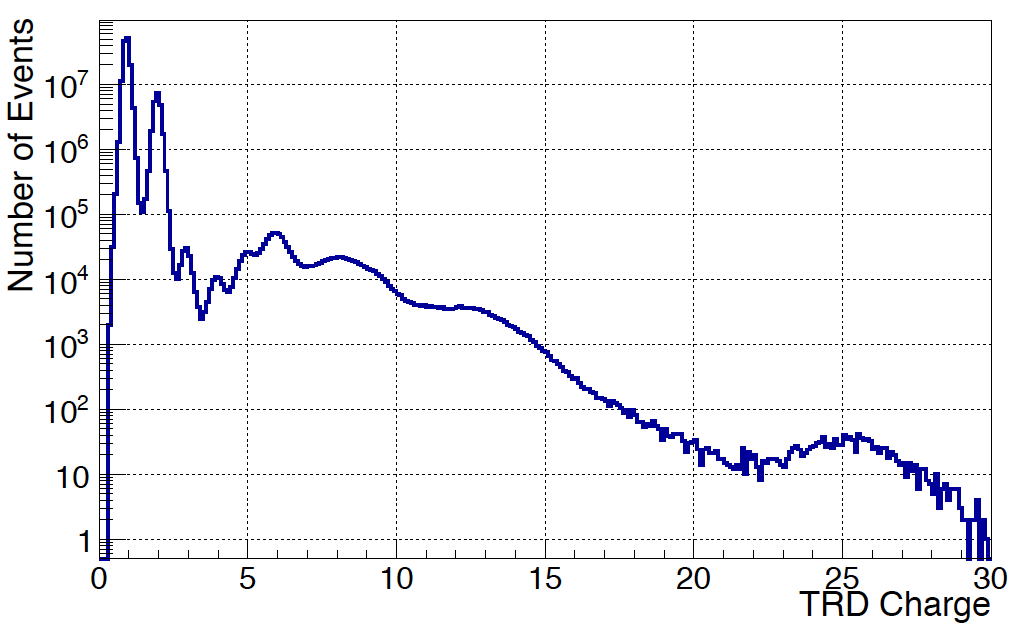
\includegraphics[width=0.9\textwidth]{TRD-ChargeMeas.png}
				
				%\scriptsize{\bluetextbf{Figure 1:}}\\
				\begin{columns}
					\begin{column}{0.06\textwidth}\end{column}
					\begin{column}{0.9\textwidth}
						\justifying								
						\scriptsize{\bluetextbf{Figure 1:} Distribution of charge of cosmic ray nuclei measured by the TRD alone.}
					\end{column}
					\begin{column}{0.02\textwidth}\end{column}
				\end{columns}
			\end{figure}
		\end{column}
		\begin{column}{0.04\textwidth}\end{column}
		\begin{column}{0.475\textwidth}
			\begin{figure}
				\centering
				%\small{\bluetextbf{Displacement}}
				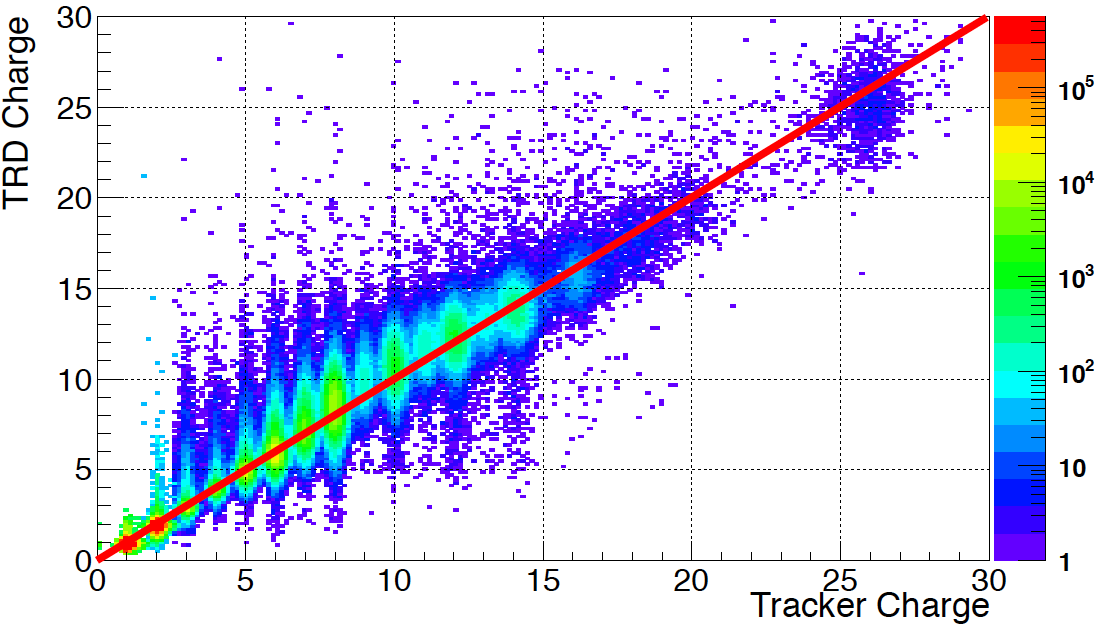
\includegraphics[width=0.9\textwidth]{TRD-ChargeMeas-Comparation.png}
				
				%\scriptsize{\bluetextbf{Figure 2:}}\\
				\begin{columns}
					\begin{column}{0.05\textwidth}\end{column}
					\begin{column}{0.9\textwidth}
						\justifying								
						\scriptsize{\bluetextbf{Figure 2:} Comparison between charge measured by the TRD and charge measured by the 
						inner Silicon Tracker.}
					\end{column}
					\begin{column}{0.05\textwidth}\end{column}
				\end{columns}
			\end{figure}
		\end{column}
		\begin{column}{0.015\textwidth}\end{column}
	\end{columns}
	
	\vspace{0.3cm}
	\small{The performance studied from ISS flight data shows \textbf{heavy nuclei up to Fe can be identified}.}
	
\end{frame}

\subsection{ToF}
\begin{frame}
	\frametitle{ToF - Time of Flight}
	\justifying

%    \vspace*{-0.25cm}
	
	\begin{columns}
		\begin{column}{0.05\textwidth}\end{column}
		\begin{column}{0.44\textwidth}\centering
			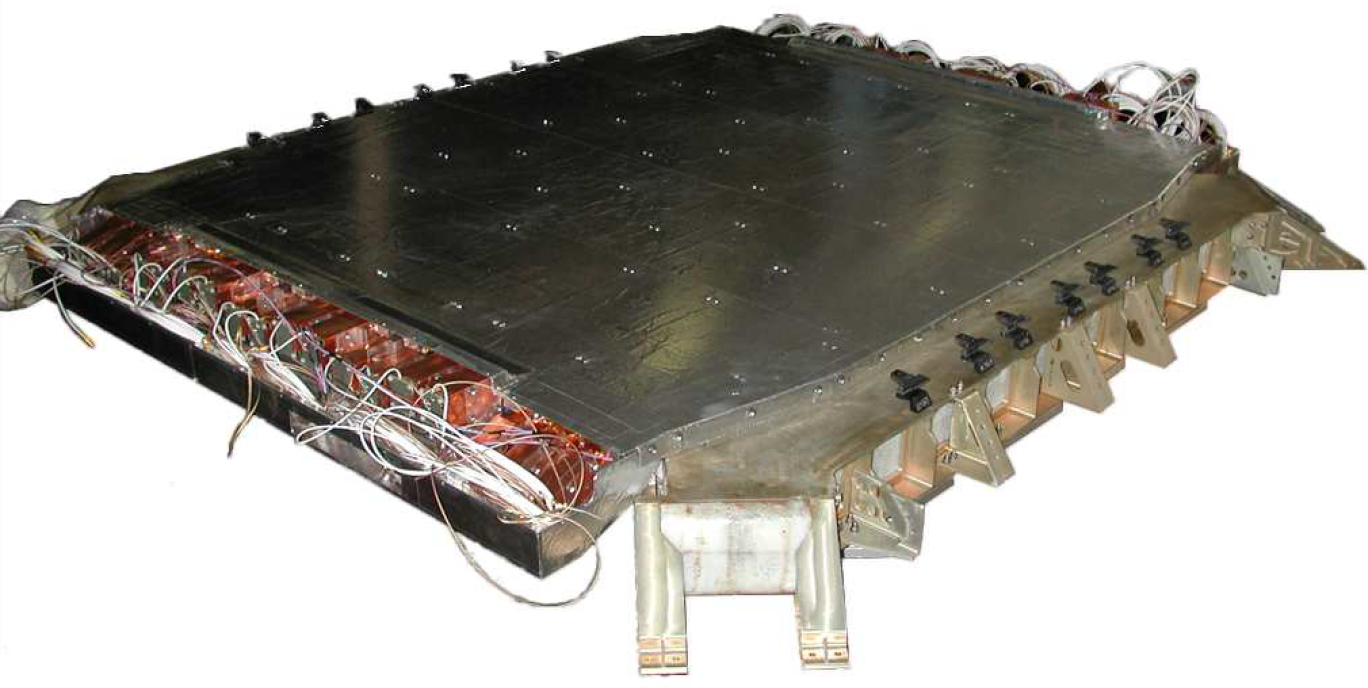
\includegraphics[width=\columnwidth]{ToF-Photo-UToF-02.png}
		\end{column}
		\begin{column}{0.02\textwidth}\end{column}
		\begin{column}{0.44\textwidth}\centering
			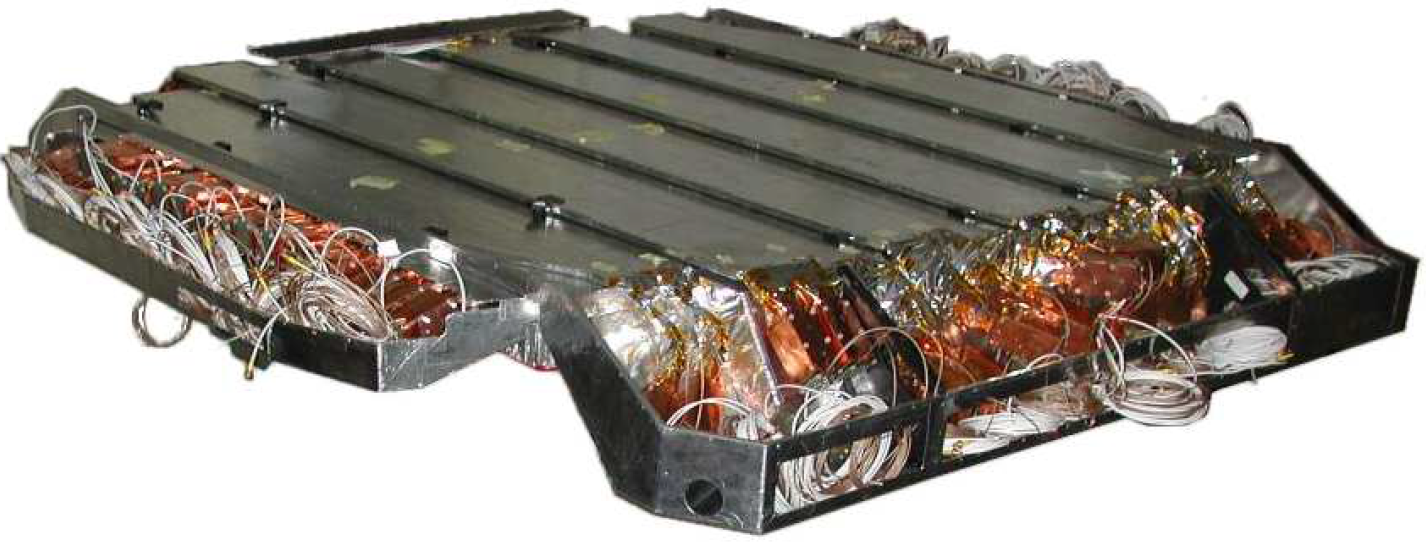
\includegraphics[width=\columnwidth]{ToF-Photo-LToF-02.png}
		\end{column}
		\begin{column}{0.05\textwidth}\end{column}
	\end{columns}
	
	\vspace*{0.1cm}		
		
	\begin{columns}
		\begin{column}{0.13\textwidth}\end{column}
		\begin{column}{0.74\textwidth}\justifying
			\scriptsize{\bluetextbf{Figure:} The completed upper and lower ToF before the final shielding.}
		\end{column}
		\begin{column}{0.13\textwidth}\end{column}
	\end{columns}
	
	%\vspace*{-0.45cm}
	
	\begin{block}{\small{The ToF system has been completely designed and built to provide:}}
		%\vspace{-0.25cm}
		\begin{itemize}\justifying
		\small{
			\item	The \textbf{fast trigger} to the experiment.
			%\vspace{-0.05cm}
			\item	The \textbf{measurement of the time-of-flight} of the particles traversing the detector with a resolution 
						sufficient \textit{to distinguish}:
						\vspace{-0.05cm}
						\begin{itemize}\justifying
							\item[$\circ$]	\textit{upward from downward going particles} at a level of $10^{-9}$;
							\item[$\circ$]	\textit{anti-protons from electrons} up to about $1.2 GeV$.
						\end{itemize}
			%\vspace{-0.05cm}
			\item 	The \textbf{measurement of primary cosmic nuclei velocity}, with a resolution of a few percent, \textbf{and of 
						their absolute charge} up to at least $Z = 15$.
		}
		\end{itemize}
	\end{block}
	%\scriptsize{\footnotetext[1]{\justifying This is based on previous experience and well-established techniques.}}
\end{frame}

\begin{frame}
	\frametitle{ToF - Time of Flight}
	\framesubtitle{parameters taken into account while designing the ToF detector}
	\justifying
	
	\footnotesize{The main parameters taken into account have been the following:}
	
	\begin{itemize}
		\justifying
		\footnotesize{
		\item[$\circ$]	\bluetextbf{Total sensitive area -}
								AMS-02 has been designed to have a large acceptance for cosmic ray tracks. To match the full acceptance 
								of the magnet, each layer of the ToF system has to cover a circular area of about $1.6 m^2$.
		\item[$\circ$]	\bluetextbf{Trigger selection -}
								A particle able to traverse the Upper and Lower ToF is said to be inside to the AMS acceptance. In this case 
								the ToF alerts all the AMS sub-detectors and data from Tracker, TRD, RICH, ECAL, ACC and ToF itself are 
								collected, processed and stored.
		\item[$\circ$]	\bluetextbf{Weight -}
								Given the limitations in the total weight of AMS, the TOF system was allotted $268 kg$ 
								to accommodate for the detector it self and for the support structure.
		\item[$\circ$]	\bluetextbf{Power consumption -}
								The TOF system was allowed to use about $150 W$ for photomultiplier tube operation and signal read-out, 
								out of the $2 kW$ electric power given by NASA to the AMS experiment on the ISS. 
		\item[$\circ$]	\bluetextbf{Time-of-flight resolution -}
								A resolution in the ToF better than $180 ps$ is needed to satisfy the physics requirements. The choice 	was 
								$1 cm$ thick scintillator, as a compromise between the minimum thickness and the light output needed to 
								reach this resolution.
		}
	\end{itemize}	
\end{frame}


\begin{frame}
	\frametitle{ToF - Time of Flight}
	\framesubtitle{the scintillation counters of the ToF detector}
	\justifying
	
	\small{The \textbf{ToF system consists of two planes of scintillator paddles}: the first situated at the entrance of the 
	magnetic volume, the second one at the exit.
	
	Distance from the magnet: $\pm 626 mm$ - distance between the two planes:
	$120 cm$. 
	
	\textbf{Each plane contains two layers of counters}, in x and y directions, respectively.}
	
	\vspace*{-0.2cm}
	\begin{center}
		%\scriptsize{\bluetextit{Top view of the upper (left) and lower (right) ToF paddles during an assembly test.}}
		%\vspace{0.1cm}
		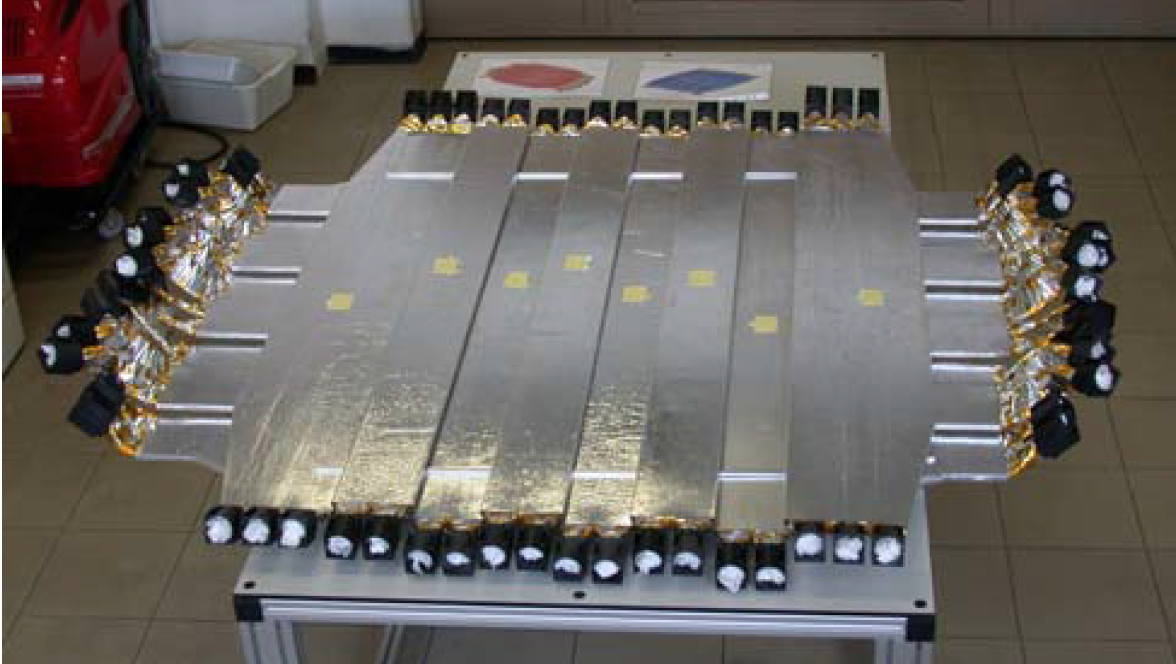
\includegraphics[height=0.25\paperheight]{ToF-Photo-UToF.png}
		\hspace*{0.1cm}
		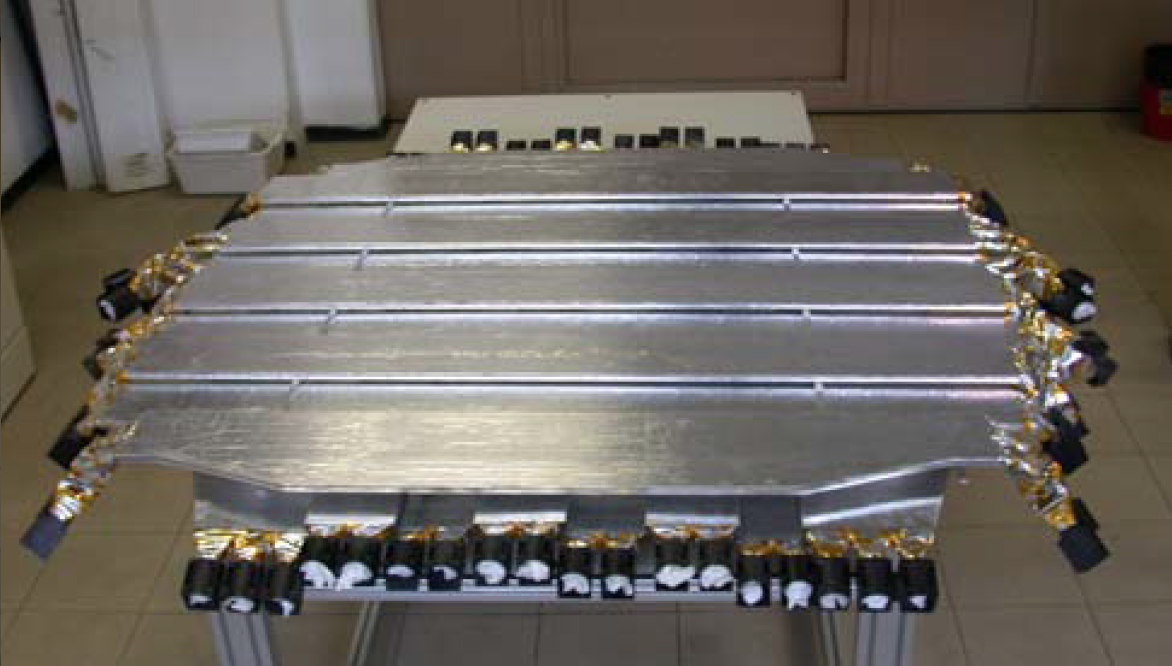
\includegraphics[height=0.25\paperheight]{ToF-Photo-LToF.png}

		\vspace*{0.1cm}		
		
		\begin{columns}
			\begin{column}{0.1\textwidth}\end{column}
			\begin{column}{0.8\textwidth}\justifying
				\scriptsize{\bluetextbf{Figure (}\bluetextit{from left to right}\bluetextbf{):}  top view of the upper (layer 1 and 2) and 
								lower (layer 3 and 4) ToF planes during an assembly test. These planes are called \textit{UToF} and 
								\textit{LToF}, respectively.}
			\end{column}
			\begin{column}{0.1\textwidth}\end{column}
		\end{columns}
	\end{center}	
	
	\vspace*{-0.2cm}
	\small{Mechanical constraints, due to the support structures of the other AMS-02 detectors, required a \textbf{different 
	design for the UToF}, mechanically connected to the TRD, \textbf{and for the LToF} mechanically connected to the Unique 
	Support Structure.}
\end{frame}

\begin{frame}[label=ToF-Paddles]
	\frametitle{ToF - Time of Flight}
	\framesubtitle{a ToF paddle}
	\justifying
	
	\small{The four ToF layers have, respectively, from the first to the last: 8, 8, 10 and 8 paddles (a paddle consists of a 
	polyvinyltoluene EJ-200 scintillator).}
	\vspace*{-0.3cm}
	
	\begin{columns}
		\begin{column}{0.25\textwidth}\end{column}
		\begin{column}{0.5\textwidth}
			\begin{figure}
				\centering

				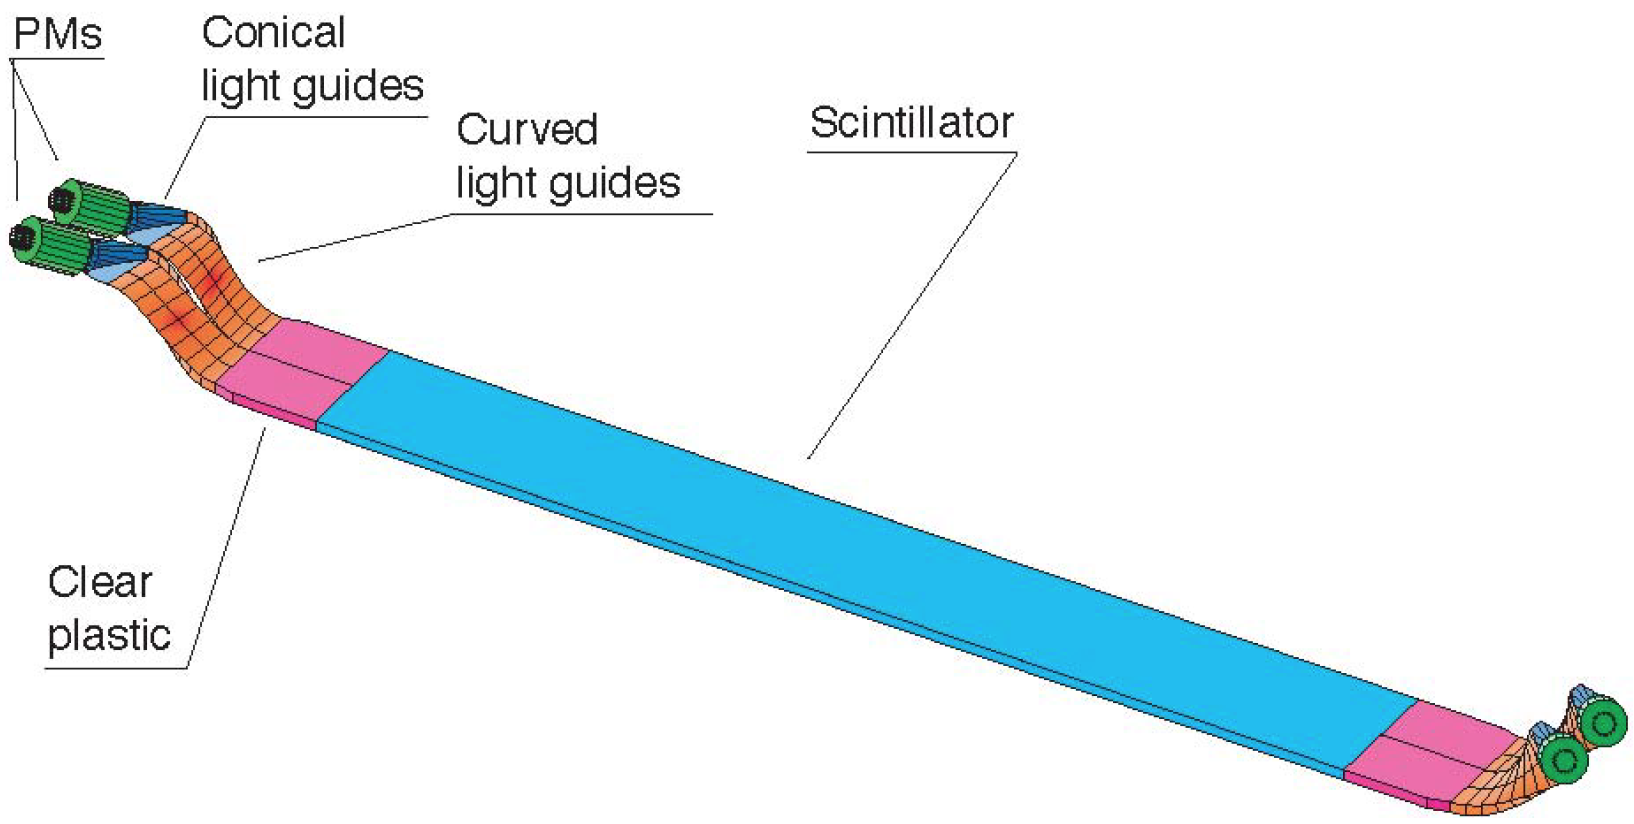
\includegraphics[width=\textwidth]{ToF-Paddle-01.png}
			\end{figure}
		\end{column}
		\begin{column}{0.25\textwidth}\end{column}
	\end{columns}	
		\begin{columns}
		\begin{column}{0.1\textwidth}\end{column}
		\begin{column}{0.8\textwidth}
			\begin{figure}		
				\centering
				\vspace*{-0.4cm}
				\scriptsize{\bluetextbf{Figure:}
				Design of a TOF paddle.}
			\end{figure}
		\end{column}
		\begin{column}{0.1\textwidth}\end{column}
	\end{columns}	

	\vspace{0.25cm}
	\small{The internal paddles, of a layer, have a rectangular shape, $1 \, cm$ thick, $12 \, cm$ width and $110 \div 135 \, cm$ 
	length, while the external counters have a trapezoidal shape with $18 \div 26 \, cm$ width and $110 \, cm$ length.
	To ensure $100 \%$ trigger efficiency, neighbouring counters are overlapped by $0.5 \, cm$.}	
	
%	\begin{columns}
%		\begin{column}{0.02\textwidth}\end{column}
%		\begin{column}{0.44\textwidth}
%			\begin{figure}
%				\centering
%				\vspace*{-0.15cm}
%
%				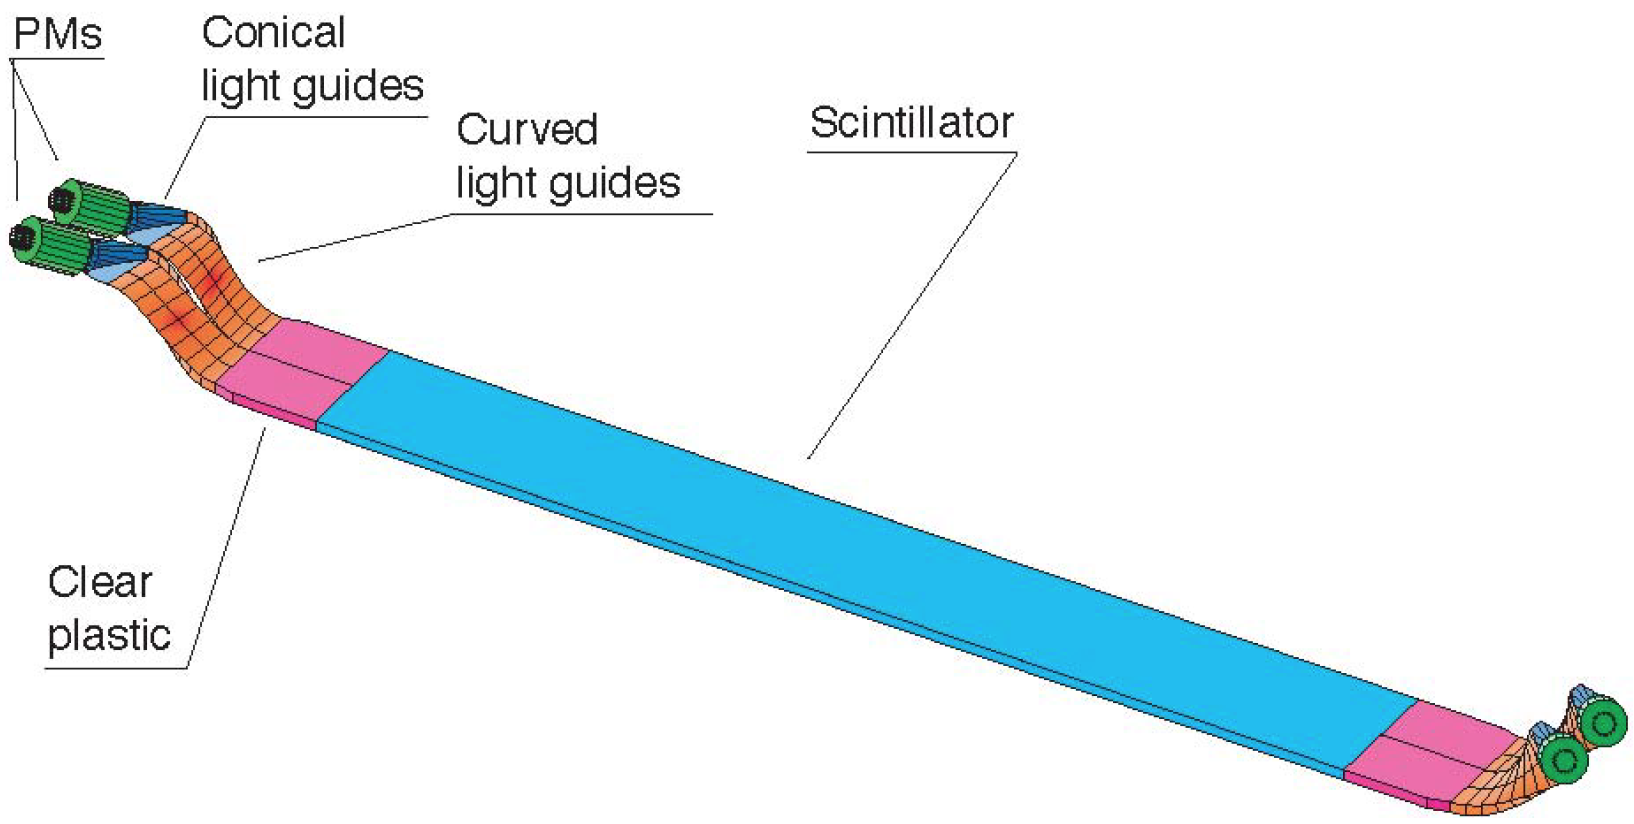
\includegraphics[width=\textwidth]{ToF-Paddle-01.png}
%				%\vspace*{0.1cm}
%			\end{figure}
%		\end{column}
%		\begin{column}{0.01\textwidth}\end{column}
%		\begin{column}{0.45\textwidth}\justifying
%			\vspace*{0.5cm}
%			
%			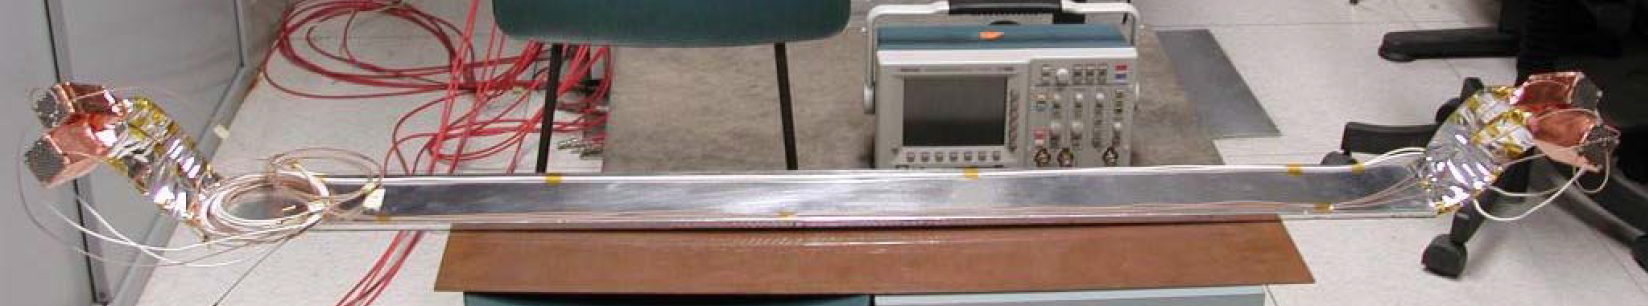
\includegraphics[width=\textwidth]{ToF-Paddle-02.png}
%			
%			\vspace{0.2cm}\scriptsize{\bluetextbf{Figures:}
%			
%			 Design of a TOF paddle (on the left) and photograph of an assembled paddle (on the top).}
%		\end{column}
%		\begin{column}{0.02\textwidth}\end{column}
%	\end{columns}	
	
	\vspace*{0.2cm}	\hfill	
	\hyperlink{ToF-CADpannels}{\textbf{\beamerbutton{more on EJ-200 scintillator}}}
	\hspace{-0.1cm}
	\hyperlink{ToF-CADpannels}{\textbf{\beamerbutton{more on ToF planes design}}}
\end{frame}

\begin{frame}
	
	Each side of a ToF counter is connected to 2 or 3 R5946 Hamamatsu Photo-Multiplier Tubes (PMTs)\footnotemark[2] through plexiglass light guides. 
	The light guides can be straight, tilted or tilted and twisted to minimize the effect of magnetic field on the PMT signal. 
	The 144 photomultipliers, connected to the 34 TOF paddles, are powered by 4 power supply (Scintillator High Voltage, SHV), which can provide a voltage between $1700 V$ and $2250 V$. The nominal gain of the photomultipliers is about $10^6$ when powered at $2000 V$.
	
	The PMTs fine-mesh R5946 Hamamatsu have been chosen for their capability of working in high magnetic fields, while keeping good timing characteristics.

\end{frame}

\begin{frame}
	The long term operational reliability of the TOF system is assured by its modular design. 
	Every counter is read at both sides by at least two photomultiplier tubes and it can still trigger with only one tube working. 
	The same is true for the (unlikely) complete failure of one counter, as the normal trigger logic requires a signal in three layers out of four. 
	In this way, the system is fault tolerant and somewhat redundant by design.
	
	%The powering and read-out electronics are protected with conformal coating from the highly ionizing low-orbit space environment and passed qualification tests to verify the absence of sparks, discharges or leakage. 
	The one per one redundant design ensures constant operation even in case of a hardware failure in the power supplies or in the read-out electronics.
\end{frame}


\begin{frame}{Others sub-system of the AMS-02 experimet}{}
	\begin{itemize}
		\item	\textitem{ACC}{Anti-Coincidence Counter}, rejects CRs traversing the magnet walls.
		\item	\textitem{TAS}{Tracker Alignment System}, checks the Tracker alignment stability.
		\item	\bluetextbf{Star Tracker and GPS}, defines the position and orientation of the AMS-02 experiment.
		\item	\bluetextbf{Electronics}, transform the signals detected by the various particle detectors into digital information to be analysed by computers.
	\end{itemize}
\end{frame}


\section{Bibliography}
\begin{frame}[allowframebreaks]
	\frametitle{Bibliography}
	\justifying
		
	\bluetextbf{General information on the AMS-02 experiment:}
	
	\begin{thebibliography}{99}
	\setbeamertemplate{bibliography item}[text]
	\scriptsize{
	\bibitem{Ting} 
	S. Ting, ``\textit{The Alpha Magnetic Spectrometer on the International Space Station}'' Nuclear Physics B (Proc. Suppl.) 
	243-244 (2013) 12–24
	
	\bibitem{Kounine} 
	A. Kounine, ``\textit{THE ALPHA MAGNETIC SPECTROMETER ON THE INTERNATIONAL SPACE STATION}'' Int. J. Mod. Phys. E, 
	21, 1230005 (2012).
	
	\bibitem{AMSCollab}
	AMS Collaboration, ``\textit{AMS on ISS - Construction of a particle physics detector on the International Space Station}'' AMS 
	Internal Note.
	
	\bibitem{Duranti}
	M. Duranti, ``\textit{Measurement of the Atmospheric Muon Flux on Ground with the AMS-02 Detector}'' PhD thesis, University 
	of Perugia	(2011)
		
	\bibitem{Vagelli}
	V. Vagelli, ``\textit{Measurement of the cosmic $e^+ + e^-$ Flux from 0.5 GeV to 1 TeV with the Alpha Magnetic 
	Spectrometer (AMS-02) on the International Space Station}'' PhD thesis, Karlsruher Institut f\"{u}r Technologie (2014).
	
	\bibitem{AMS-website}
	AMS Collaboration, ``\textit{AMS-02 - The Alpha Magnetic Spectrometer Experiment}'' \url{http://www.ams02.org/}
	}

	\framebreak
	\hspace{-0.7cm}\normalsize{\bluetextbf{On the Transition Radiation Detector (TRD):}}		
	
	\scriptsize{
	\bibitem{Kirn-1}
	T. Kirn, ``\textit{The AMS-02 transition radiation detector}'' Nuclear Instruments and Methods in Physics Research A 581 
	(2007) 156–159.
	
	\bibitem{Kirn-2}
	T. Kirn, ``\textit{The AMS-02TRDontheinternationalspacestation}'' Nuclear Instruments and Methods in Physics Research A 
	706 (2013) 43–47.
	
	\bibitem{Sun}
	W. Sun, A. Kounine and Z. Weng, ``\textit{Measurement of the absolute charge of cosmic ray nuclei with the AMS Transition 
	Radiation Detector}'' 33rd International Cosmic Ray Conference, Rio de Janeiro (2013).
	}
	
	\vspace{0.25cm}
	\hspace{-0.7cm}\normalsize{\bluetextbf{On the Time of Flight detector (ToF):}}
	
	\scriptsize{
	\bibitem{Bindi-1}
	V. Bindi et al., ``\textit{The scintillator detector for the fast trigger and time-of-flight (TOF) measurement of the space 
	experiment AMS-02}'' Nuclear Instruments and Methods in Physics Research A 623 (2010) 968–981.
	
	\bibitem{Bindi-2}
	V. Bindi et al., ``\textit{The AMS-02 time of flight (TOF) system: construction and overall performances in space}'' 33rd 
	International Cosmic Ray Conference, Rio de Janeiro (2013).
	
	\bibitem{Bindi-3}
	V. Bindi et al., ``\textit{Calibration and performance of the AMS-02 time of flight detector in space}'' Nuclear Instruments and 
	Methods in Physics Research A 743 (2014) 22–29.
	}
	\end{thebibliography}
\end{frame}

\appendix
\setbeamertemplate{footline}
{
	\leavevmode%
	\hbox{%
  		% "ht" è lo spazio sopra il carattere partendo dalla base del carattere, "dp"  è lo spazio sotto il carattere partendo sempre dalla base del carattere
  		\begin{beamercolorbox}[wd=.333333\paperwidth,ht=2.5ex,dp=1ex,left,leftskip=4ex]{author in head/foot}%
   			\usebeamerfont{author in head/foot}\insertshortauthor
  		\end{beamercolorbox}%
  		\begin{beamercolorbox}[wd=.333333\paperwidth,ht=2.5ex,dp=1ex,center]{institute in head/foot}%
    		\usebeamerfont{title in head/foot}\insertshortinstitute
 		 \end{beamercolorbox}%
 		 \begin{beamercolorbox}[wd=.333333\paperwidth,ht=2.5ex,dp=1ex,right,rightskip=4ex]{date in head/foot}%
 		 	\usebeamerfont{date in head/foot}\insertshortdate{}\hspace*{0.3cm}(insights)
 		 \end{beamercolorbox}
 		 }%
 	\vskip0pt%
}

%% POSSIBILI SLIDE SULLA TERIA DELLA RADIAZIONE DI TRANSIZIONE
\begin{frame}<presentation:0>[label=TR-details,noframenumbering]
	\frametitle{TRD - Transition Radiation Detector}
	\framesubtitle{Transition Radiation - Angular Distribution\hspace{4.35cm}\hyperlink{TRD-main}{\beamerbutton{back to TRD}}}
	\justifying
	\footnotesize{
	The frequency spectrum of TR emitted by a particle with charge $Z e$ upon perpendicular traversal through a single interface 
	between two media with dielectric constants $\epsilon_f$ and $\epsilon_g$ has been calculated by Ginzburg and Frank and
	by Garibian. These calculations show that for highly relativistic particles most of the radiation is emitted in the x-ray region.}
	
	\vspace{-0.39cm}
	%\vspace{0.05cm}
	
	\begin{columns}
		\begin{column}{0.01\textwidth}\end{column}
		\begin{column}{0.51\textwidth}
			\justifying
		
			%\vspace{-0.4cm}
			\footnotesize{

			In this case $\epsilon_{f,g} \simeq 1 - \omega_{f,g}^2/\omega^2$ and the expression for the 
			\textbf{differential radiation intensity} is:
		
			\vspace{-0.15cm}
			$$ \frac{dW}{d(\hbar \omega) \: d\theta} = \frac{2 Z^2 \alpha}{\pi} f_0(\theta) $$				
		
			\vspace{0.1cm}
			
			where $\omega_{f,g}$ are the plasma frequencies of the two media, i.e.:
			 
			 \vspace{-0.4cm}
			$$ \omega_{f,g} = 28.8 \: \sqrt{\rho_{f,g} \, \frac{Z_{f,g}}{A_{f,g}}} \: eV $$
		
			with $\rho_{f,g}$ that are the densities of the two materials, $Z_{f,g}$ the atomic numbers and $A_{f,g}$ the 
			atomic weights.
			}
		\end{column}
		\begin{column}{0.48\textwidth}
			\centering
			\vspace{0.45cm}
			
			\hspace{0.25cm}\scriptsize{\bluetextit{Angular distribution of a single surface yield.}}	
			
			\vspace{0.05cm}			
			
			\begin{columns}
				\begin{column}{0.03\textwidth}\end{column}
				\begin{column}{0.9\textwidth}
					\centering
					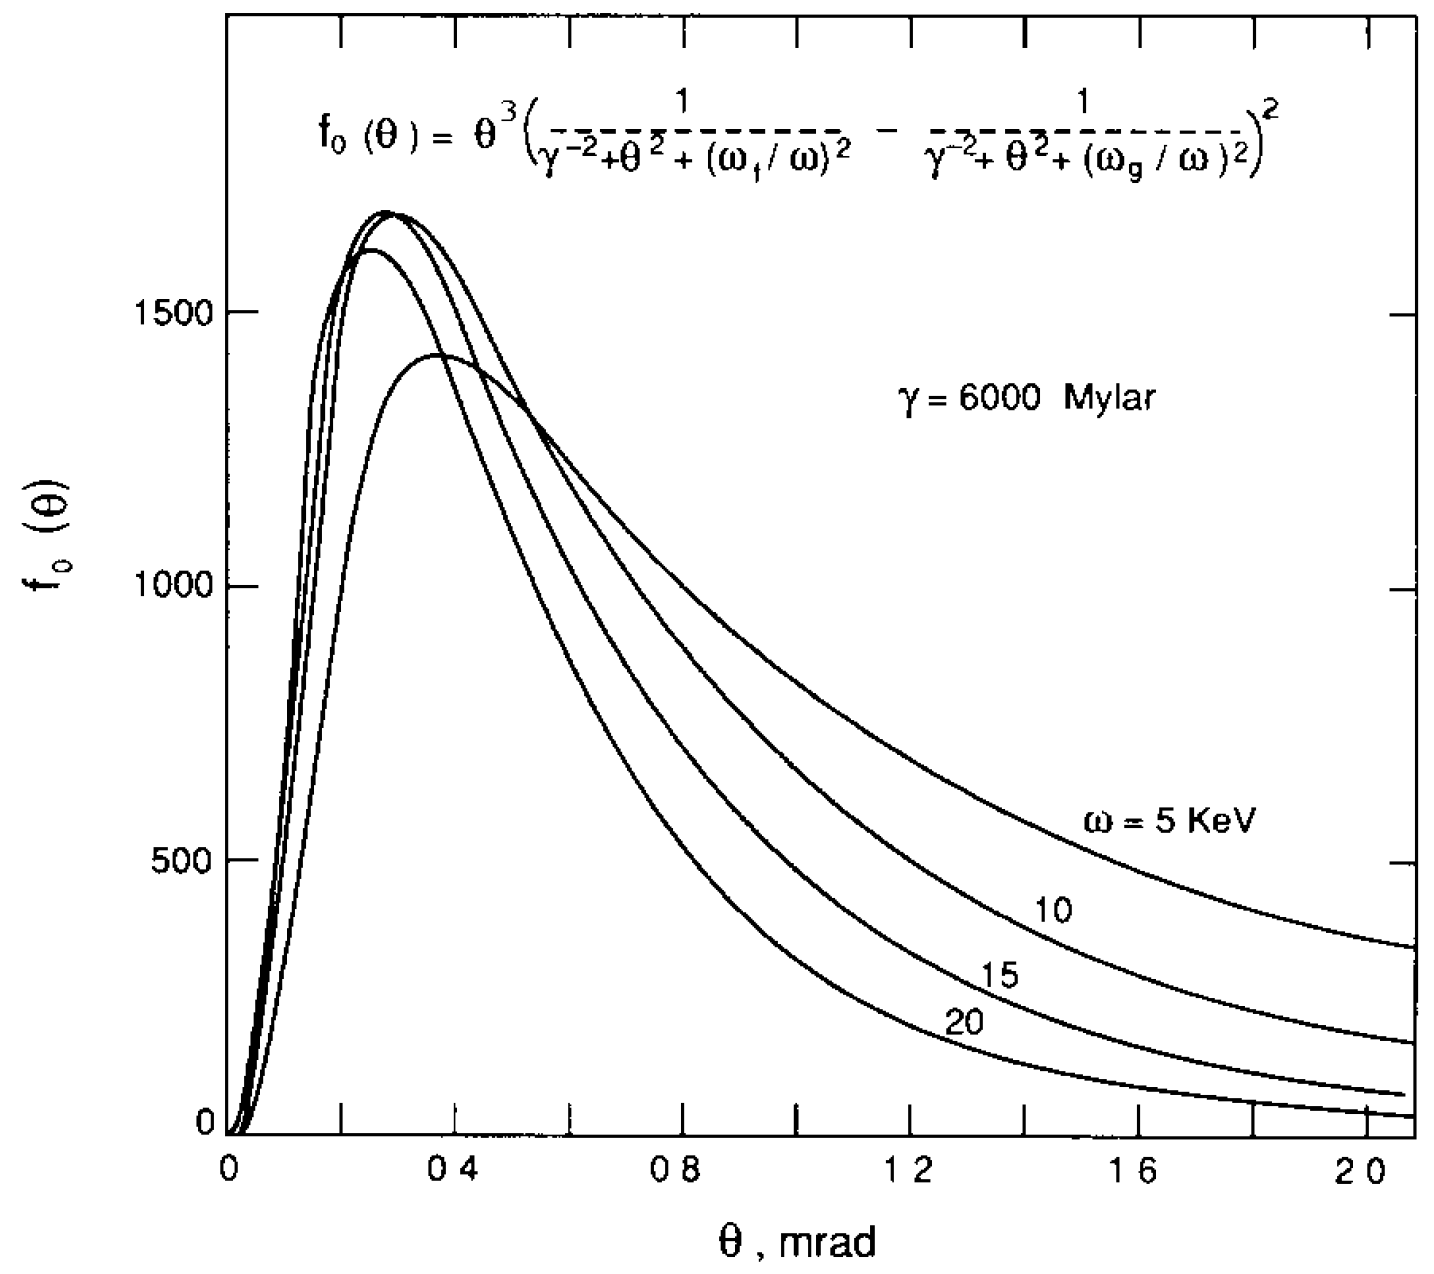
\includegraphics[width=\textwidth]{TR-AngularDistr.png}		
				\end{column}
				\begin{column}{0.07\textwidth}\end{column}
			\end{columns}												
		\end{column}
		\begin{column}{0.01\textwidth}\end{column}
	\end{columns}
\end{frame}

\begin{frame}<presentation:0>[noframenumbering]
	\frametitle{TRD}
	\framesubtitle{Transition Radiation - Angular Distribution\hspace{4.35cm}\hyperlink{TRD-main}{\beamerbutton{back to TRD}}}
	\justifying
	
	\footnotesize{The distribution has a peak at the narrow angle $\theta \simeq \gamma^{-1}$ and extends to the angle of order
	$\sqrt{\gamma^{-2} + \omega_f^2 / \omega^2}$.
	Because the TR angle  $\theta \simeq \gamma^{-1}$ is very small, the practical application of the angle measurements is very 
	difficult.}
		
	\vspace{-0.5cm}
	\begin{columns}
		\begin{column}{0.01\textwidth}\end{column}
		\begin{column}{0.32\textwidth}
			\begin{figure}
				\centering
				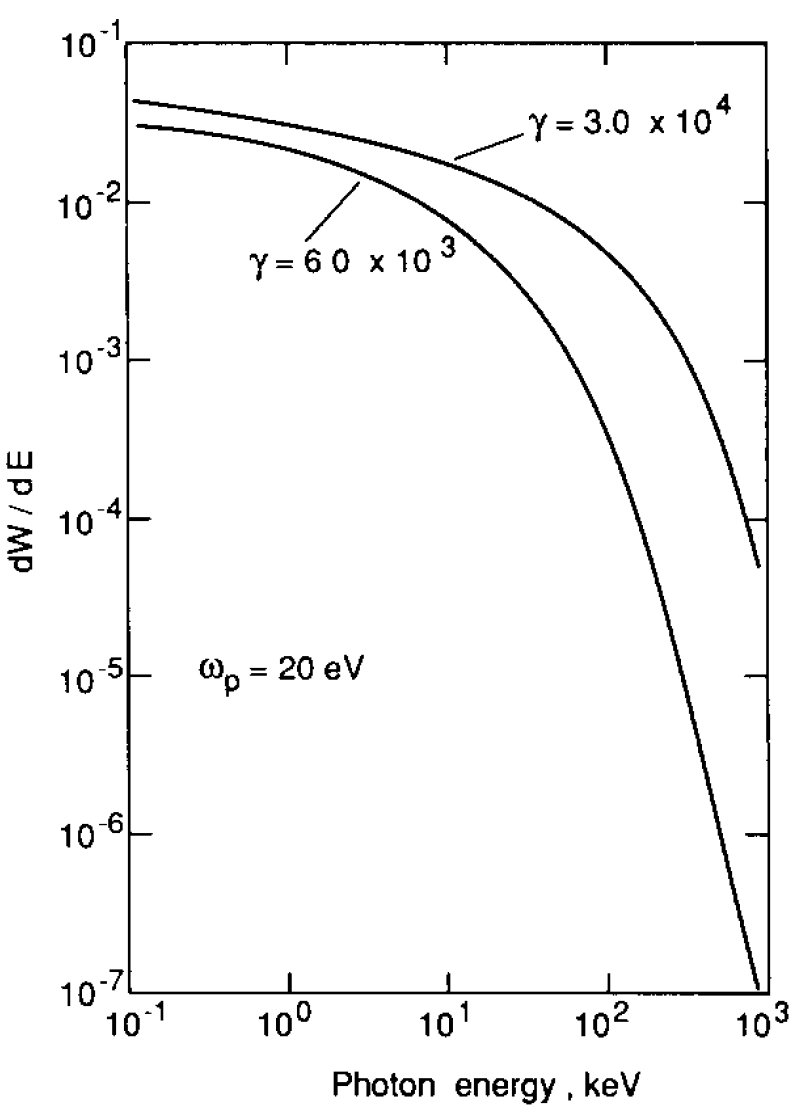
\includegraphics[width=\textwidth]{TR-EnergySpecrum.png}
				
				%\scriptsize{\bluetextbf{Figure:} The radiated TR spectrum from a polyethylene surface}
			\end{figure}
		\end{column}
		\begin{column}{0.67\textwidth}
		\justifying
		
		\footnotesize{
		The integration of $dW/(\hbar d\omega \: d\theta)$ respect to $\theta$ yields the energy spectrum: 
		\begin{equation*} 
		\frac{dW}{d(\hbar \omega)} = \frac{Z^2 \alpha}{\pi} \left[ \frac{\omega_f^2 + \omega_g^2 + 2 \omega^2 \gamma^{-2}}{\omega_f^2-\omega_g^2}	\ln \left( \frac{\omega^2 \gamma^{-2} + \omega_f^2}{\omega^2 \gamma^{-2} + \omega_g^2} \right) - 2 \right]
	\end{equation*}
		and, integrating this spectrum in $\hbar d\omega$, the total radiation intensities is obtained, namely:
\begin{equation*}
		W \simeq Z^2 \cdot \frac{\hbar \alpha}{3} \cdot \frac{(\omega_f - \omega_g)^2}{\omega_f + \omega_g} \gamma \propto Z^2 \cdot \frac{E}{m c^2}
	\end{equation*}		
%	The differential energy spectrum can be broken up in essentially three regions having respectively, constant, logarithmic, and power-law dependence on $\omega$ and $\gamma$
%		\begin{equation*}
%		\frac{dW}{d\omega} \simeq 
%		\left\{
%		\begin{array}{ll}
%		\frac{2 Z^2 \alpha \hbar}{\pi}  \left( \ln \frac{\omega_f}{\omega_g} - 1 \right) \quad \quad \omega < \gamma \omega_g
%		\vspace{0.15cm}\\
%		\frac{2 Z^2 \alpha \hbar}{\pi}  \ln \frac{\omega_f}{\omega} \quad \quad \quad \quad \quad \gamma \omega_g < \omega < \gamma \omega_f \vspace{0.15cm}\\
%		\frac{Z^2 \alpha \hbar}{6 \pi}  \left( \frac{\omega_f}{\omega} \right)^4 \quad \quad \quad \quad \quad \gamma \omega_f < \omega
%		\end{array}
%		\right.
%	\end{equation*}
		}
		\end{column}
		\begin{column}{0.01\textwidth}\end{column}
	\end{columns}
		
		
\end{frame}

\begin{frame}<presentation:0>[noframenumbering]
	\begin{equation*} 
		\frac{dW}{d(\hbar\omega)} = \frac{Z^2 \alpha}{\pi} \left[ \frac{\omega_f^2 + \omega_g^2 + 2 \omega^2 \gamma^{-2}}{\omega_f^2-\omega_g^2}	\ln \left( \frac{\omega^2 \gamma^{-2} + \omega_f^2}{\omega^2 \gamma^{-2} + \omega_g^2} \right) - 2 \right]
	\end{equation*}
	
	\begin{equation*}
		\frac{dW}{d\omega} \simeq 
		\left\{
		\begin{array}{ll}
		\frac{2 Z^2 \alpha \hbar}{\pi}  \left( \ln \frac{\omega_f}{\omega_g} - 1 \right) \quad \quad \omega < \gamma \omega_g
		\vspace{0.15cm}\\
		\frac{2 Z^2 \alpha \hbar}{\pi}  \ln \frac{\omega_f}{\omega} \quad \quad \quad \quad \quad \gamma \omega_g < \omega < \gamma \omega_f \vspace{0.15cm}\\
		\frac{Z^2 \alpha \hbar}{6 \pi}  \left( \frac{\omega_f}{\omega} \right)^4 \quad \quad \quad \quad \quad \gamma \omega_f < \omega
		\end{array}
		\right.
	\end{equation*}
	
	\begin{equation*}
		W_{TR} \simeq Z^2 \cdot \frac{\hbar \alpha}{3} \cdot \frac{(\omega_f - \omega_g)^2}{\omega_f + \omega_g} \gamma \propto Z^2 \cdot \frac{E}{m c^2}
	\end{equation*}
	\begin{equation*}
		\theta_{TR} \lesssim \gamma^{-1}
	\end{equation*}
	\begin{equation*}
		D_{f} \simeq \frac{2 c}{\omega \left( \gamma^{-2} + \theta_{TR}^2 + \xi^2 \right)}
	\end{equation*}
\end{frame}



\begin{frame}[label=TRD-Module,noframenumbering]
	\frametitle{TRD - Transition Radiation Detector}
	\framesubtitle{photo of a radiator and a straw module}%\hspace{4.125cm}\hyperlink{TRD-Design}{\beamerbutton{back to TRD design}}}
	\begin{center}
		\vspace{-0.1cm}
		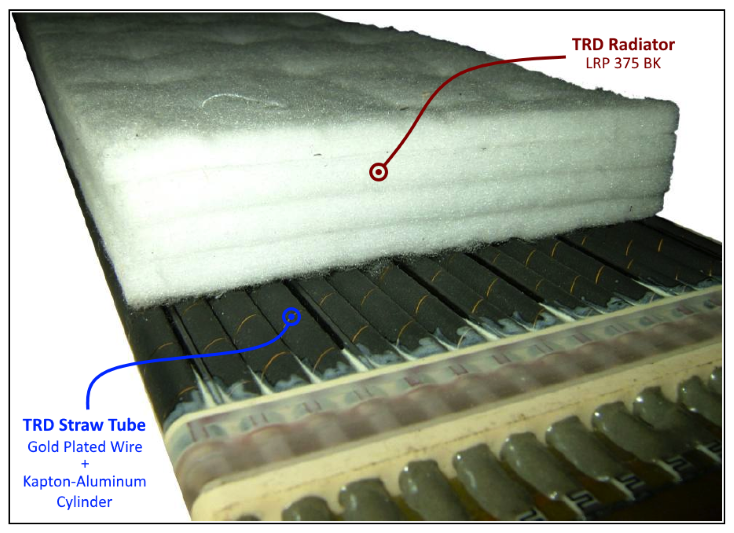
\includegraphics[height=0.65\paperheight]{TRD-RadEStraws-02mid.png}
	\end{center}
	
	\vspace{-0.1cm}\hfill\hyperlink{TRD-Design}{\beamerbutton{back to TRD design}}
\end{frame}



\begin{frame}[label=TRD-Mech_Struct,noframenumbering]
	\frametitle{TRD - Transition Radiation Detector}
	\framesubtitle{mechanical structure \hspace{6.85cm}\hyperlink{TRD-Supp_Struct}{\beamerbutton{back to TRD design}}}
	\begin{center}
		\vspace{-0.32cm}
		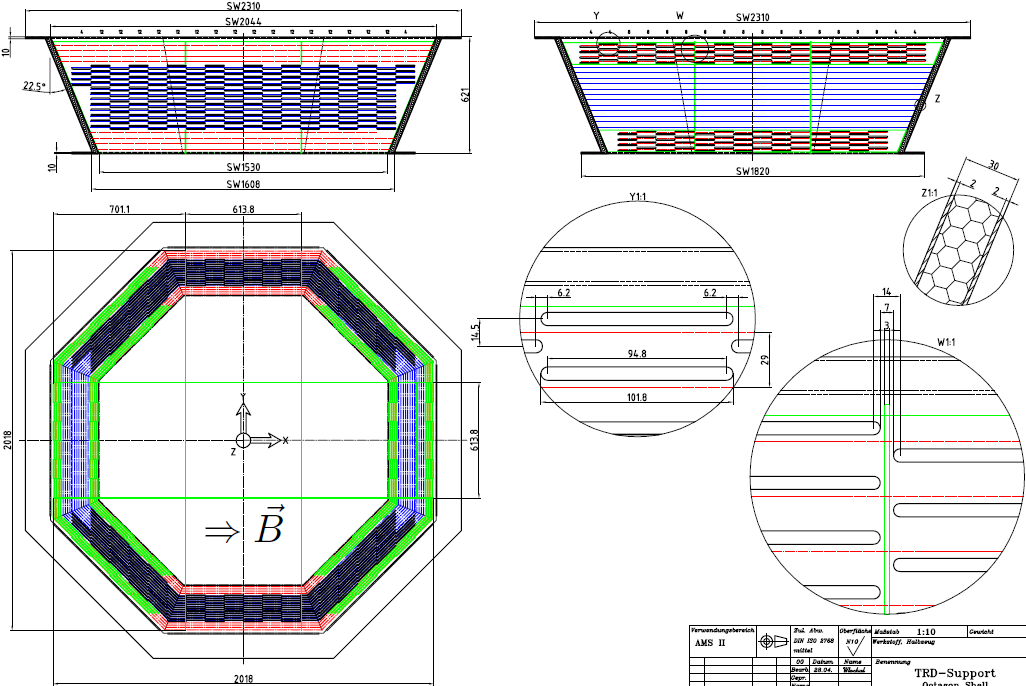
\includegraphics[height=0.775\paperheight]{TRD-Struct-04.png}
	\end{center}
\end{frame}



\begin{frame}[label=TRD-SpaceQual,noframenumbering]
	\frametitle{TRD - Transition Radiation Detector}
	\framesubtitle{more details on the space qualification of the straw modules}
	\justifying
	
	\vspace{-0.25cm}
	\scriptsize{Space qualification tests include vibration tests to simulate a space shuttle launch and thermal-vacuum tests, as 
	well as electromagnetic interference and corona tests. Gasgain and gastightness of the straw modules has 
	been	monitored during these tests.}
	
	\begin{itemize}
		\justifying
		\scriptsize{
		\item	For the \bluetextbf{vibration test}, a test jigg with 4 modules with a maximum length of $659 \, mm$ was used. 
					The test was performed on a vibration table, test cycles include a sine sweep $(0.5 \, g)$ from 10 to $2000 \, Hz$ 
					to	determine the first eigenfrequency of the structure, a random spectrum with a mean acceleration of $6.8 \, g$ to 
					simulate launch or landing with a space shuttle, and a second sine sweep to verify the first eigenfrequency has not 
					changed after performing the random  spectrum. 
					The test results show no such change. The measured first eigenfrequency of a module (length: $40 \, cm$) is 
					$f_0 = 128.5 \, Hz$. 
					A Comparison of this result with a FEC\footnotemark[1] coupled load modal analysis 	show good agreement.
		\item	For the \bluetextbf{thermal-vacuum test}, the same 4-layer test jigg has been inserted into a thermal-vacuum 
					tank at the MPE\footnotemark[2].
					During 70 hours, 9 thermocycles have been performed, with temperatures ranging from $-40 \: ^\circ{C}$ to
					$+60 \: ^\circ{C}$. 
					The test jigg was kept in vacuum at $10^{-6} mbar$. After thermal cycling, the 4 modules of the jigg were tested
					again 	for gastightness and gasgain, with no significant changes in both values.
		}
	\end{itemize}

	\hfill\hyperlink{TRD-SQ_StrawsMod}{\textbf{\beamerbutton{back to the previous slide}}}
	\footnotetext[1]{\scriptsize{Finite Elements Calculation}}
	\footnotetext[2]{\scriptsize{Max-Planck-Institut fur Extraterrestrische Physik, Munchen, Germany}}
\end{frame}


\begin{frame}[label=TRD-DeltaTech1,noframenumbering]
	\frametitle{TRD - Transition Radiation Detector}
	\framesubtitle{delta rays technique - 1}%\hspace{2.8cm}
%			\hyperlink{TRD-ChargePerform1}{\textbf{\beamerbutton{back to TRD performance}}}
%			\hspace{0.1cm}\hyperlink{TRD-DeltaTech2}{\textbf{\beamerbutton{more about this technique}}}
%			}
	\justifying
	\vspace{-0.15cm}
	\small{When charged particles pass through the TRD, the produced $keV$ scale delta rays travel almost perpendicular to the particle velocity, and some of them can be detected by the drift tubes not passed by the ions but in the vicinity (a few $cm$) of the particle track. 
	These tubes are tagged as \textit{delta ray tubes}, whereas the tubes passed by ions are defined as $dE/dx$ \textit{tubes}. 
	The signals in \textit{delta ray tubes} are typically far below the ADC saturation threshold. Particles with higher $Z$ corresponds to more delta rays, hence a higher ADC signal in \textit{delta ray tubes}.}

	\vspace{-0.35cm}
	\begin{columns}
		\begin{column}{0.05\textwidth}\end{column}
		\begin{column}{0.55\textwidth}
			\begin{figure}
				\centering
				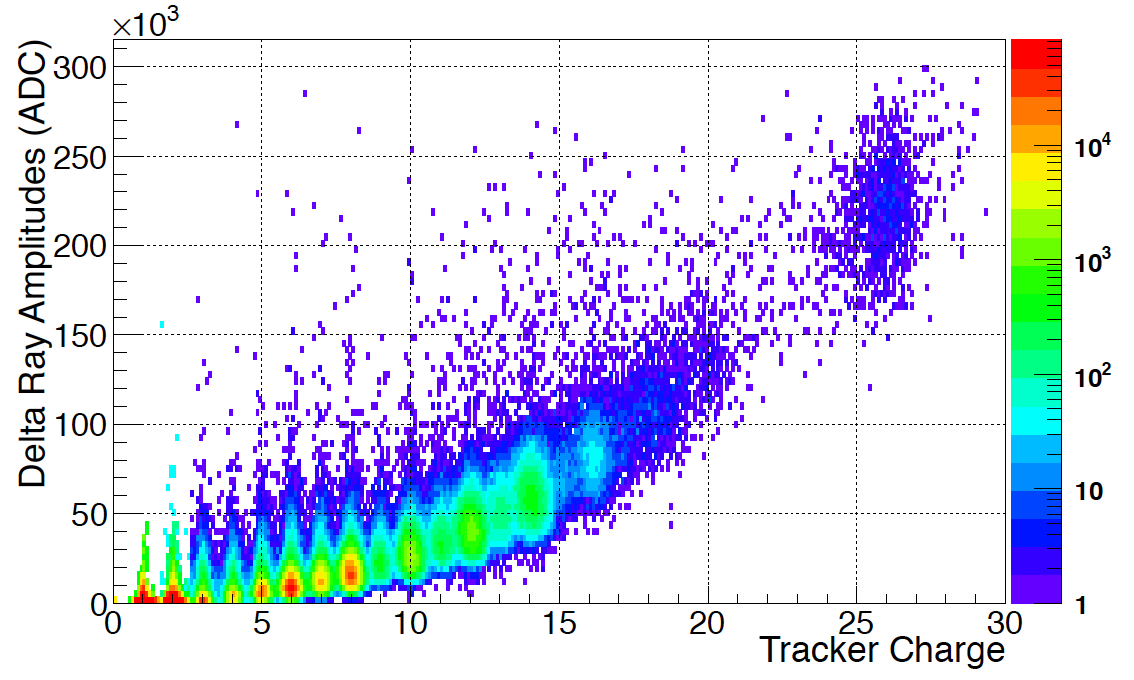
\includegraphics[width=0.95\textwidth]{TRD-ChargeMeas-DeltaAmpl.png}
				
				%\footnotesize{\caption{\justifying AAA}}
			\end{figure}
		\end{column}
		\begin{column}{0.35\textwidth}\justifying
			
			\vspace{0.1cm}
			\footnotesize{\bluetextbf{Delta ray amplitudes}}
			
			\footnotesize{Figure shows the average signal in delta ray tubes as a function of charge measured by the Silicon 
			Tracker. Clear differences of signals between different ion species can be seen.}
		\end{column}
		\begin{column}{0.05\textwidth}\end{column}
	\end{columns}

%	\begin{columns}
%		\begin{column}{0.05\textwidth}\end{column}
%		\begin{column}{0.9\textwidth}
%			\begin{figure}
%				\centering				
%				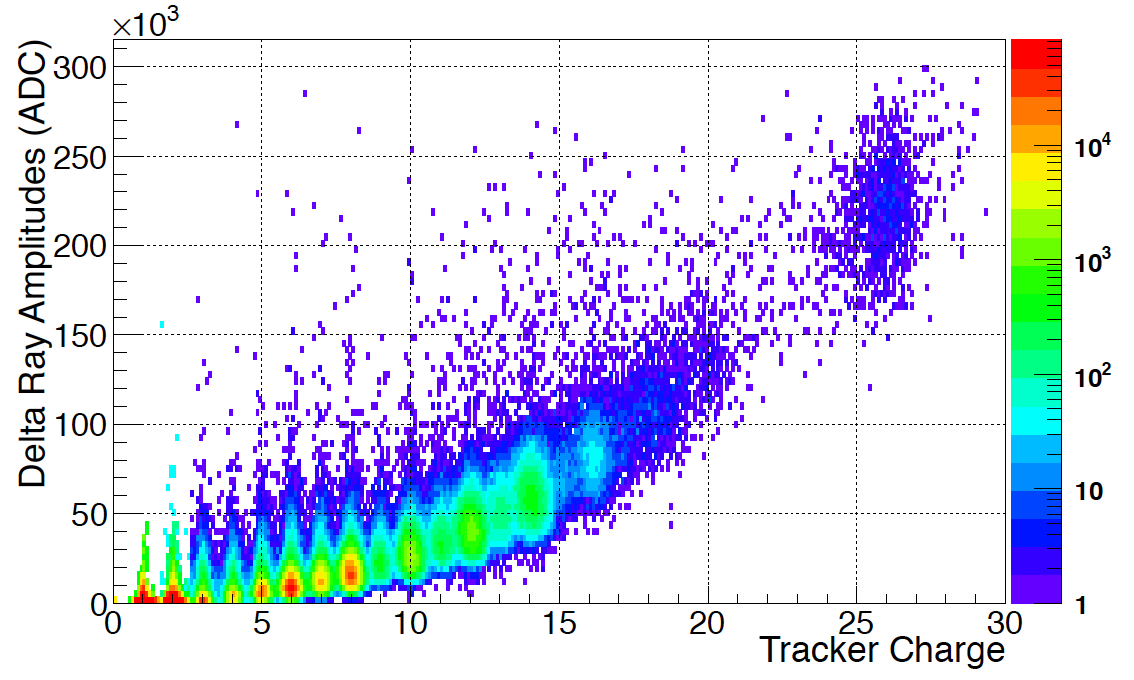
\includegraphics[height=0.3\paperheight]{TRD-ChargeMeas-DeltaAmpl.png}
%			\end{figure}
%		\end{column}
%		\begin{column}{0.05\textwidth}\end{column}
%	\end{columns}	
%	
%	\vspace{0.15cm}
%	\begin{columns}
%		\begin{column}{0.05\textwidth}\end{column}
%		\begin{column}{0.9\textwidth}
%			\justifying
%			\footnotesize{Figure shows the average signal in delta ray tubes as a function of charge measured by the Silicon 
%			Tracker. Clear differences of signals between different ion species can be seen.}
%		\end{column}
%		\begin{column}{0.05\textwidth}\end{column}
%	\end{columns}
%	\vspace{0.15cm}
%	\hfill\hyperlink{TRD-ChargePerform1}{\textbf{\beamerbutton{back to TRD performance}}}
%	\hspace{1ex}\hyperlink{TRD-DeltaTech2}{\textbf{\beamerbutton{more about this technique}}}

	\hfill
	\hyperlink{TRD-ChargePerform1}{\textbf{\beamerbutton{back to TRD performance}}}
	\hspace{-0.1cm}
	\hyperlink{TRD-DeltaTech2}{\textbf{\beamerbutton{more about this technique}}}
\end{frame}

\begin{frame}[label=TRD-DeltaTech2,noframenumbering]
	\frametitle{TRD - Transition Radiation Detector}
	\framesubtitle{delta rays technique - 2}%\hspace{2.8cm}
%			\hyperlink{TRD-DeltaTech1}{\textbf{\beamerbutton{back to the previous slide}}}
%			\hspace{0.1cm}\hyperlink{TRD-ChargePerform1}{\textbf{\beamerbutton{return to TRD performance}}}
%			}
	\justifying
	\small{The dependences of \textit{delta ray tube} amplitude on layer and inclination are studied and no obvious dependence is 
	found. However, the \textit{delta ray tube} amplitude does change with increasing energy of the incoming particle.}

	\vspace{-0.2cm}
	\begin{columns}
		\begin{column}{0.02\textwidth}\end{column}
		\begin{column}{0.5\textwidth}
			\begin{figure}
				\centering
				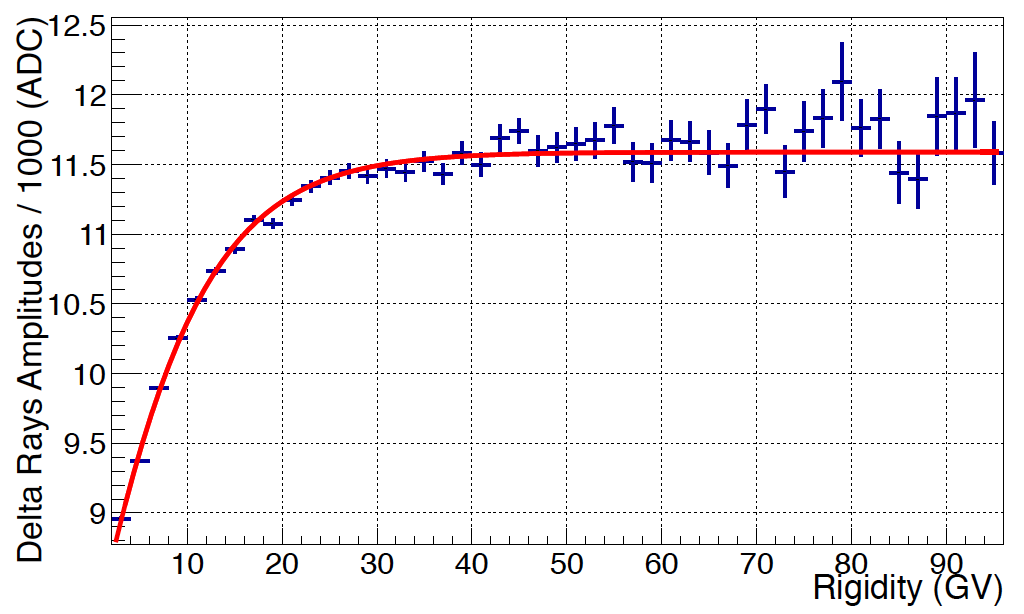
\includegraphics[width=\textwidth]{TRD-ChargeMeas-DeltaSat.png}
				
				%\footnotesize{\caption{\justifying AAA}}
			\end{figure}
		\end{column}
		%\begin{column}{0.0\textwidth}\end{column}
		\begin{column}{0.46\textwidth}\justifying
			
			\vspace{0.1cm}
			\footnotesize{\bluetextbf{Delta ray amplitudes}}
			
			\footnotesize{Plot of the amplitude as a function of rigidity for Z = 6 particles, from which we observed the number of 
			delta rays increases with rigidity for rigidity below $25 GV$, and is almost constant in higher rigidity ranges.}
		\end{column}
		\begin{column}{0.02\textwidth}\end{column}
	\end{columns}
	
	\vspace{0.2cm}
	\small{Similar to $dE/dx$ \textit{PDFs}, we get \textit{Delta Ray PDFs} by parametrization on \textit{delta ray tube} 
	amplitude distributions.}
	
%	\vspace{0.3cm}
%	\hfill\hyperlink{TRD-DeltaTech2}{\textbf{\beamerbutton{back to the previous slide}}}
%	\hspace{1ex}\hyperlink{TRD-DeltaTech2}{\textbf{\beamerbutton{return to TRD performance}}}
	\hfill
	\hyperlink{TRD-DeltaTech1}{\textbf{\beamerbutton{back to the previous slide}}}
	\hspace{-0.1cm}
	\hyperlink{TRD-ChargePerform1}{\textbf{\beamerbutton{return to TRD performance}}}
\end{frame}

\begin{frame}[label=ToF-CADpannels,noframenumbering]
	\frametitle{ToF - Time of Flight}
	\framesubtitle{scintillator counters and light guides CAD design for UToF and LToF}
	
	%\vspace*{-0.25cm}
	\begin{columns}
	\begin{column}{0.08\textwidth}\end{column}
	\begin{column}{0.4\textwidth}
		\centering
		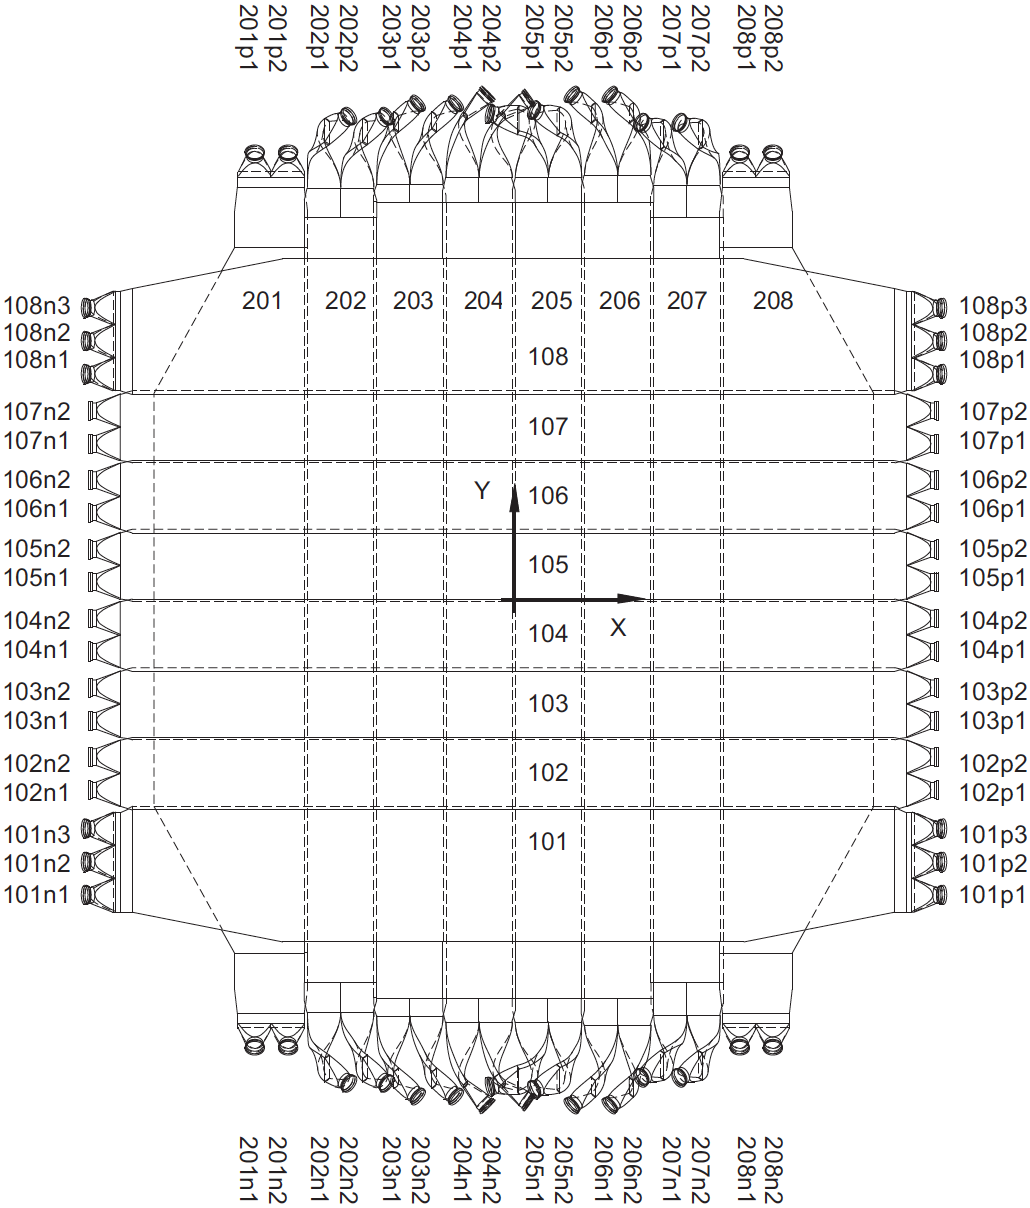
\includegraphics[height=0.58\paperheight]{ToF-PadsScheme_UToF.png}
	\end{column}
	\begin{column}{0.04\textwidth}\end{column}
	\begin{column}{0.4\textwidth}
		\centering
		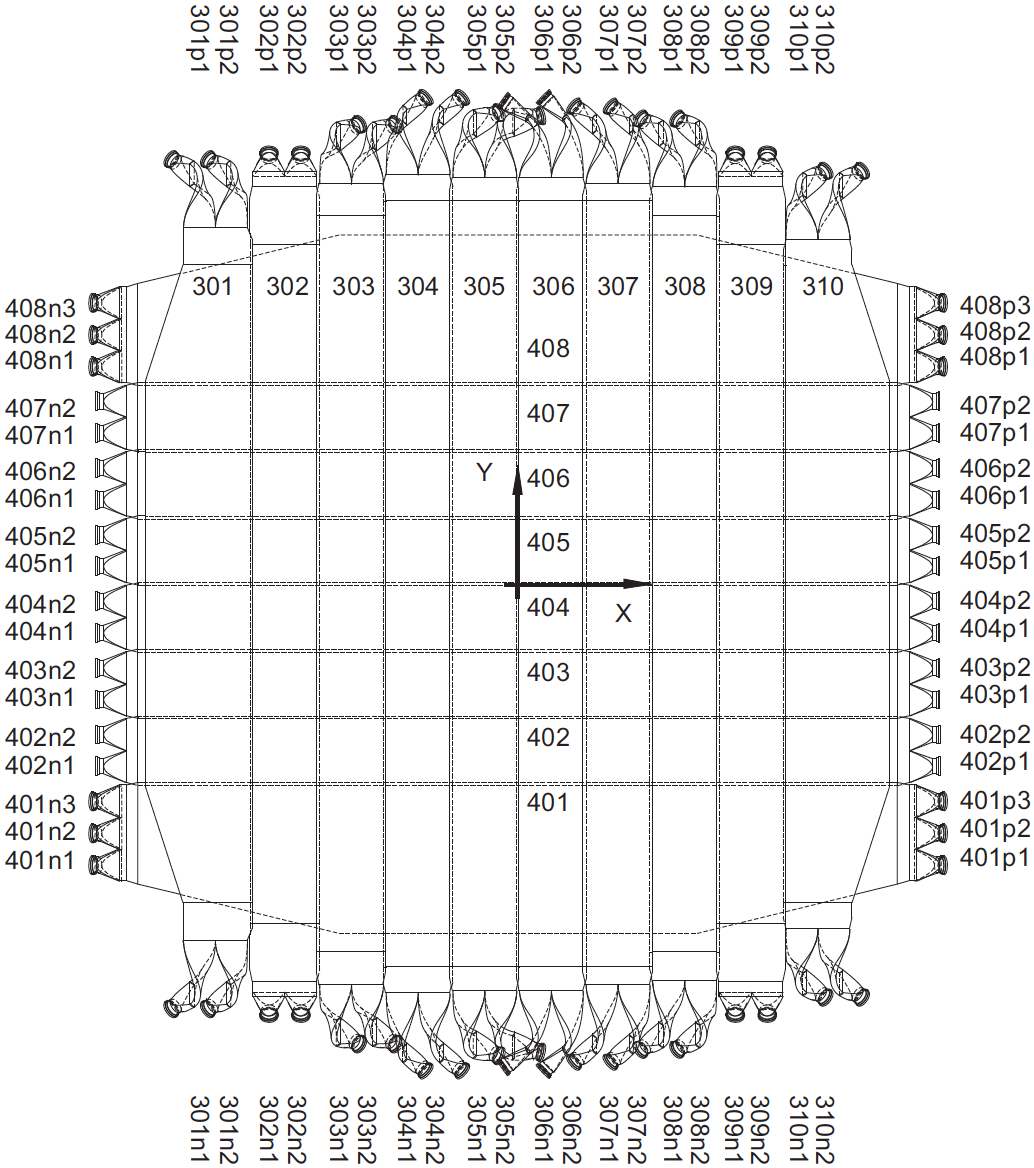
\includegraphics[height=0.58\paperheight]{ToF-PadsScheme_LToF.png}
	\end{column}
	\begin{column}{0.08\textwidth}\end{column}
	\end{columns}
	\begin{columns}
	\begin{column}{0.11\textwidth}\end{column}
	\begin{column}{0.34\textwidth}
		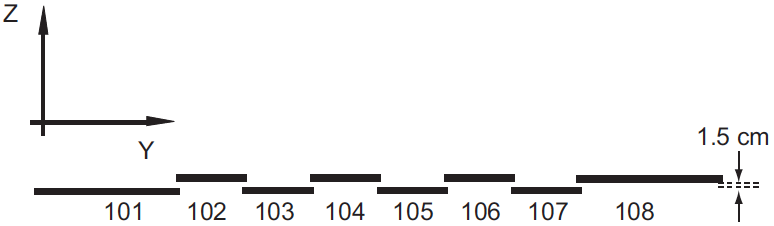
\includegraphics[width=\columnwidth]{ToF-PadsScheme_UToF-side.png}
	\end{column}
	%\begin{column}{0.01\textwidth}\end{column}
	\begin{column}{0.51\textwidth}
		\justifying
		
		\vspace*{-0.25cm}\hspace*{0.35cm}\scriptsize{\bluetextbf{Figure:}}
		\begin{itemize}\justifying
			\tiny{
			\item[$\triangleright$]	Top view of the scintillator counters and light guides CAD design for the UToF (top left) and LToF 
												(right).
			\item[$\triangleright$]	Side view of layer 1 (bottom left).
			}
		\end{itemize}
						
	\end{column}
	\begin{column}{0.04\textwidth}\end{column}
	\end{columns}
	
	\vspace*{0.1cm}\hfill
	\hyperlink{ToF-Paddles}{\textbf{\beamerbutton{back to the previous slide}}}
	\hspace{-0.1cm}
	\hyperlink{ToF-LISTpannels}{\textbf{\beamerbutton{list of all counter types}}}
\end{frame}

\begin{frame}[label=ToF-LISTpannels,noframenumbering]
	\frametitle{ToF - Time of Flight}
	\framesubtitle{counter types}
	\justifying
	\vspace*{-0.15cm}
	
	\scriptsize{List of all counter types with light guide shape, counter shape, dimensions, number of PMTs per side and efficiency 
	of the light guides computed with the simulation\footnotemark[1].}
	\vspace*{-0.3cm}
	
	\begin{center}
		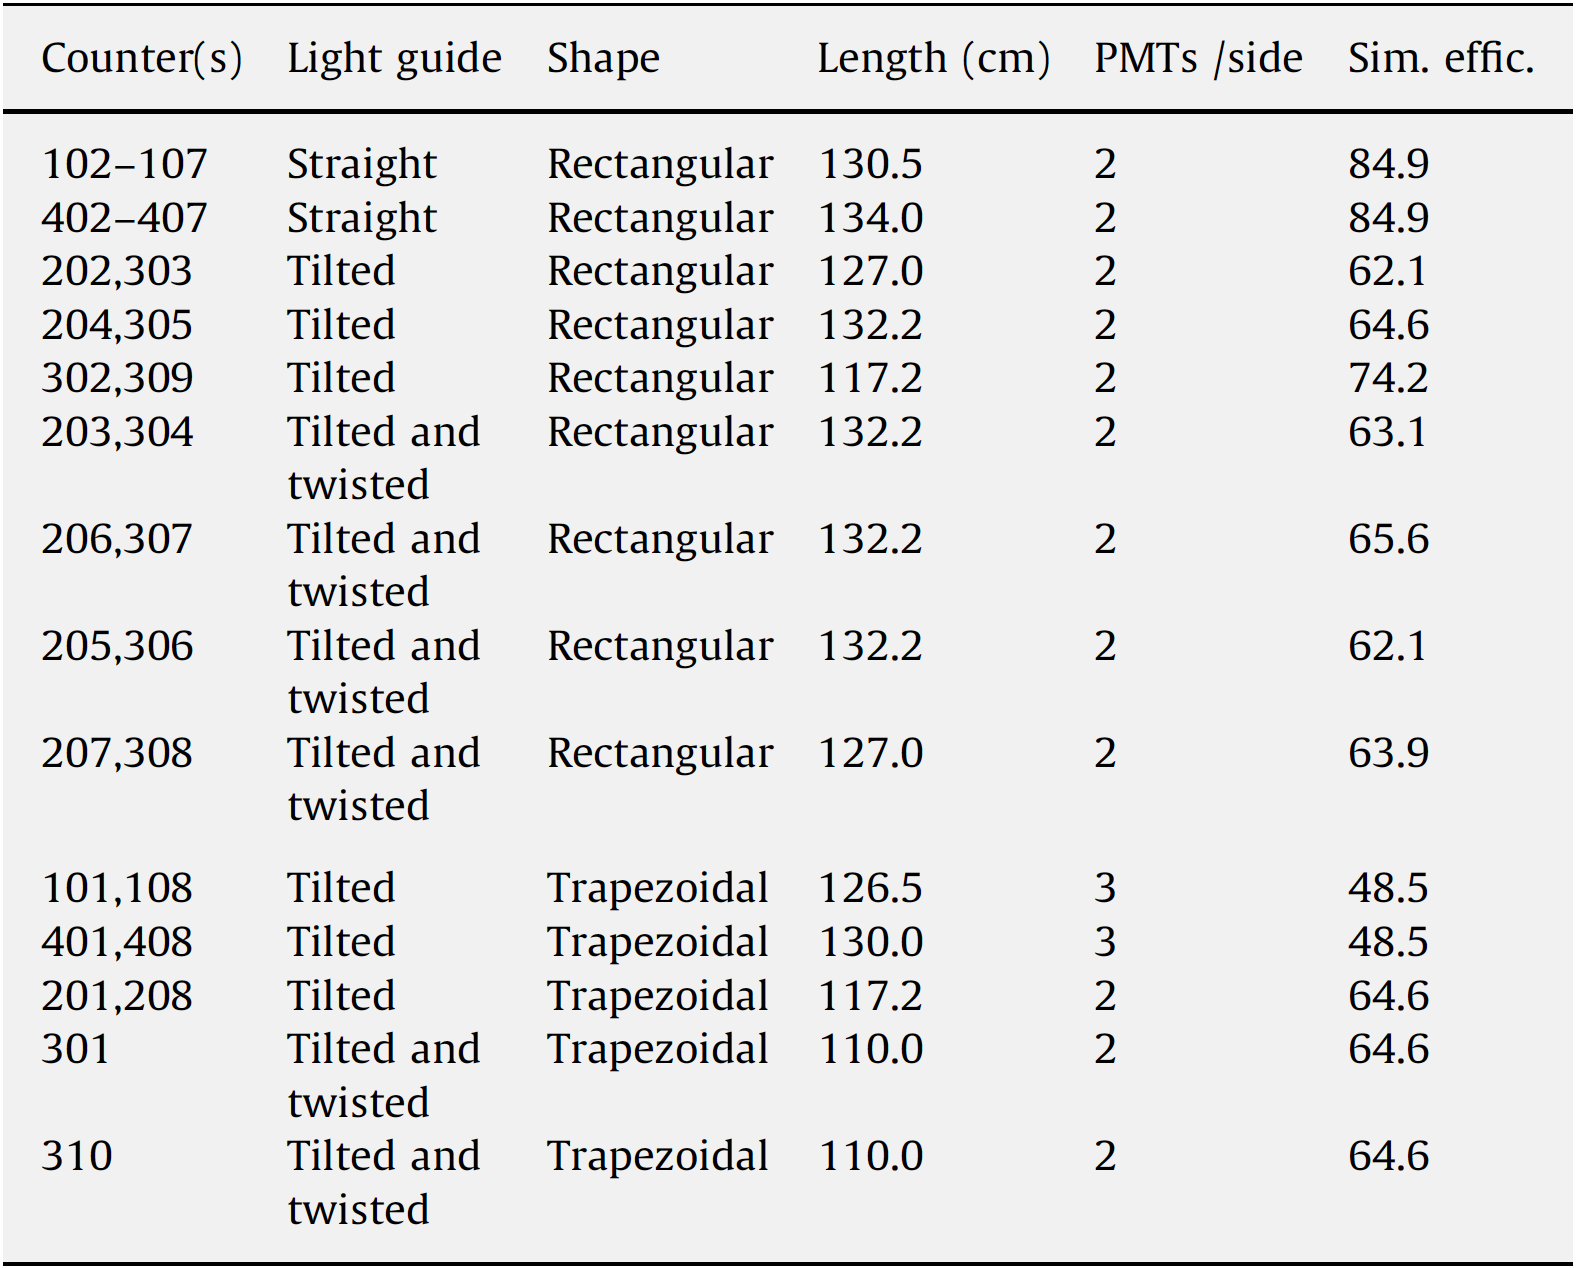
\includegraphics[height=0.505\paperheight]{ToF-ListOfCounters.png}
	\end{center}		
	\vspace*{-0.3cm}	
	
	\footnotetext[1]{\tiny{The light transmission efficiency of the 10 different light guide types was also simulated with a ray 
	tracing program taking into account the angular distribution at the light guide entrance and the angular acceptance on the 
	cathode glass window. For the trapezoidal counters, the simulation took into account also the counter geometry, therefore the 
	efficiency is much smaller than for the rectangular counters.}}
	
	\hfill	
	\hyperlink{ToF-CADpannels}{\textbf{\beamerbutton{back to the previous slide}}}
	\hspace{-0.1cm}
	\hyperlink{ToF-Paddles}{\textbf{\beamerbutton{return to the presentation}}}
\end{frame}

\begin{frame}
	\frametitle{ToF - Time of Flight}
	\framesubtitle{property of EJ-200 Plastic Scintillator}
	\justifying
	\vspace{-0.1cm}
	
	\scriptsize{EJ-200 combines the two important properties of long optical attenuation length and fast timing which make it particularly useful for time-of-flight systems using scintillators greater than one meter long. 
	%It is the detector of choice for many industrial applications, such as gauging and environmental protection, where high sensitivity and signal uniformity are critical operating requirements.
	}%\vspace{-0.2cm}
	
	\begin{columns}
		\begin{column}{0.02\textwidth}\end{column}
		\begin{column}{0.39\textwidth}
			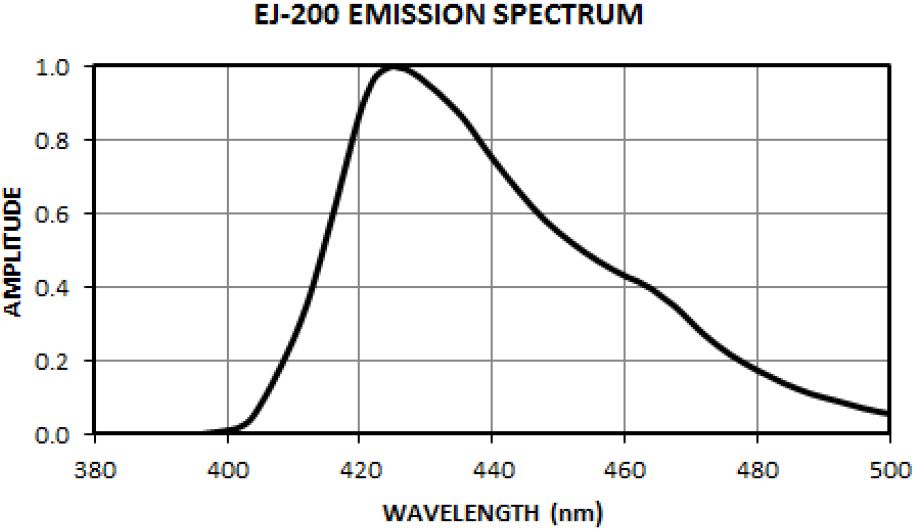
\includegraphics[width=\textwidth]{ToF-EJ200spectrum.png}
			
			\vspace*{0.1cm}
			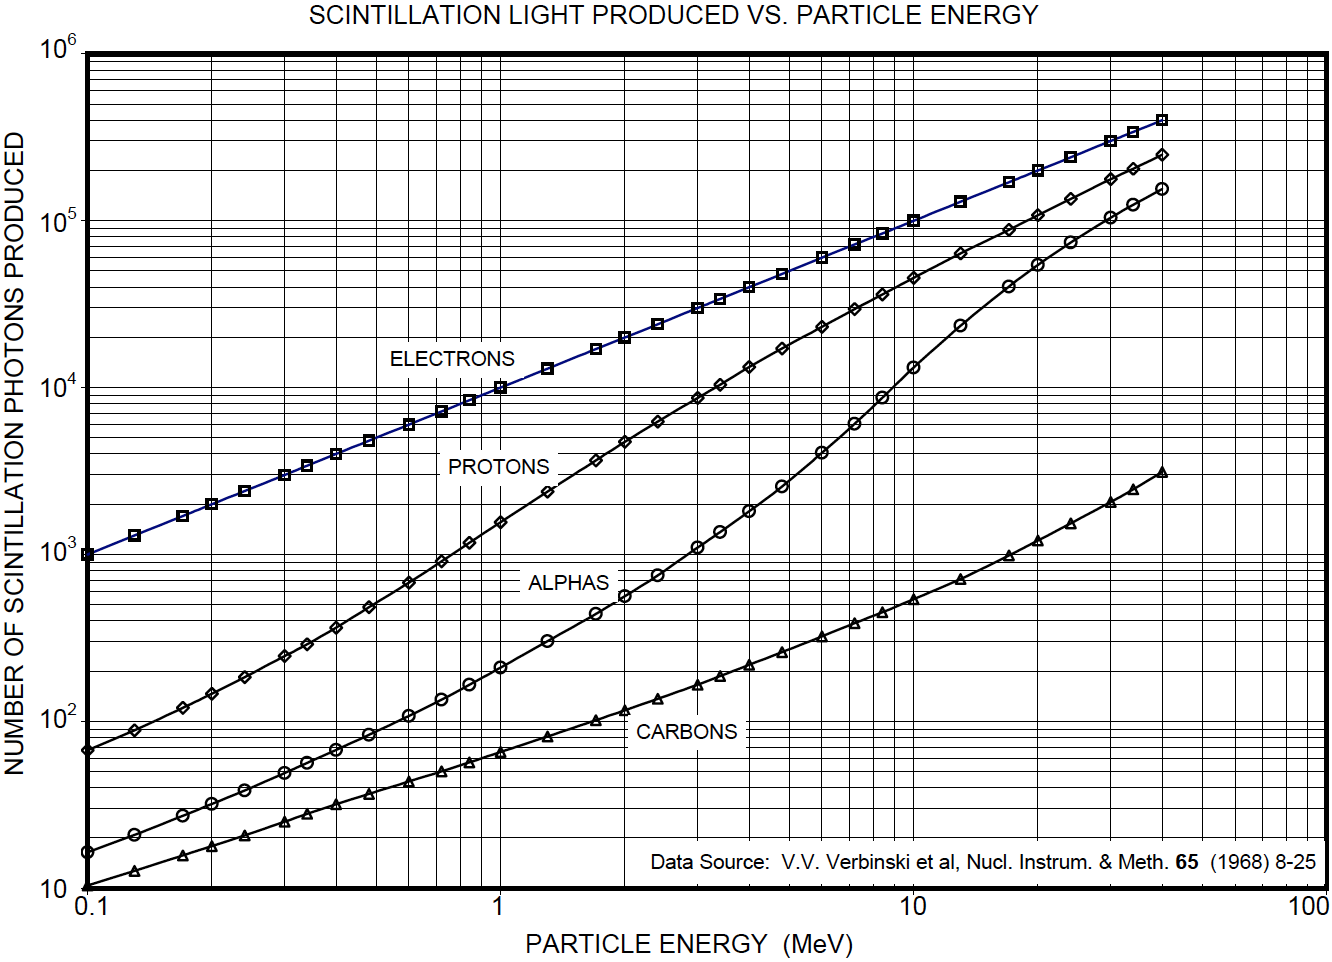
\includegraphics[width=\textwidth]{ToF-EJ200resp03.png}
		\end{column}
		\begin{column}{0.47\textwidth}
			\vspace{-0.2cm}
			\includegraphics[width=\textwidth]{ToF-EJ200prop.png}
			
			\vspace*{0.1cm}
			\includegraphics[width=\textwidth]{ToF-EJ200chem.png}
		\end{column}
		\begin{column}{0.02\textwidth}\end{column}
	\end{columns}	
	
	\vspace{-0.3cm}
	\hfill
	\hyperlink{ToF-Paddles}{\textbf{\beamerbutton{return to the presentation}}}
\end{frame}

\end{document}
